\section{Executive Summary}

\subsection{Target}

This analysis uses an innovative machine learning method to search for model-agnostic resonant new physics in the all-hadronic channel.   As the first search using these new techniques, we limit the feature space for the learning to be two-dimensional.  Future extensions will be more broadly sensitive by including more features and considering additional final states.  The analysis uses the full Run 2 dataset and targets early 2020.

\subsection{Context}

This search is complementary to existing dedicated searches for resonant new physics in the all-hadronic channel.  In particular, the analysis is similar to the inclusive dijet search~\cite{Aad:2019hjw} when the neural network cut efficiency is 100\% and is sensitive to models targeted by the all-hadronic diboson resonance search~\cite{Aad:2019fbh}.  For the former, the actual sensitivity of the ATLAS dijet search will be much weaker than our 100\% efficiency setup because they use $R = 0.4$ jets, while many of the signals targeted here are not well-captured by such small jets.  For the latter, our search will not be as sensitive when the daughter particles have masses near the Standard Model $W$ and $Z$ boson masses.  However, away from those masses, the diboson search will be largely insensitive and therefore our analysis can provide complementary coverage.  A quantitative comparison to these searches can be found in the main body of this note.  In principle, the low mass boosted dijet search (e.g. a direct search for $B$ or $C$) is also sensitive to the final states targeted in this analysis~\cite{Aaboud:2018zba,Aaboud:2018fzt,Aaboud:2019zxd,Sirunyan:2019vxa,Sirunyan:2017nvi,Sirunyan:2018ikr}.  However, those limits are order of magnitude weaker than the ones studies here and are therefore not considered further.

\subsection{Contributors}

In addition to the analysis team, we are grateful for additional contributions to the analysis: 

\begin{itemize}
\item Jack Collins: Analysis Consultant and Expert (ACE) (theorist).  Consultation on the training procedure for mitigating residual correlations.
\item Kalliopi Iordanidou: Help with running VVJJ fit.
\end{itemize}

\section{Change log}

\begin{itemize}
\item Version 0.1: Initial version, to be used for editorial board request.
\item Version 0.2: Version to be used for unblinding request (DBL approval).  v0.21 is a slight update that takes into account EB feedback.
\item Version 0.3: Full account of analysis including unblinded data. Added appendices with various auxiliary studies.
\end{itemize}

\clearpage

%-------------------------------------------------------------------------------
\section{Introduction}
\label{sec:CWoLa:intro}
%-------------------------------------------------------------------------------

The dijet resonance search is one of the first analyses performed when hadron collider reaches a new center-of-mass energy.   In particular, ATLAS has an extensive program of inclusive dijet resonance searches at $\sqrt{s}=7$~\cite{Aad:2010ae,Aad:2011aj,Aad:2011fq}, $\sqrt{s}=8$~\cite{Aad:2014aqa}, and $\sqrt{s}=13$ TeV~\cite{ATLAS:2015nsi,Aaboud:2017yvp,Aaboud:2018fzt}.  While such searches are sensitive to nearly all resonance decays to hadronic or electromagnetic objects (excluding muons), dedicated searches for particular decays will always be (much) more sensitive.  Therefore, ATLAS has an extensive program searching for di-$\tau$~\cite{Aaboud:2016cre,Aaboud:2017sjh}, di-$b$ quark resonances~\cite{Aaboud:2016nbq,Aaboud:2018tqo}, di-top quark resonances~\cite{Aaboud:2018mjh}, $bt$ resonances~\cite{Aaboud:2018juj}, di-W/Z boson resonances~\cite{Aaboud:2016okv,Aaboud:2017fgj,Aaboud:2017itg,Aaboud:2017eta}, VH resonances~\cite{Aaboud:2018eoy,Aaboud:2017cxo,Aaboud:2017ahz}, di-Higgs resonances~\cite{Aaboud:2018knk}, and many more.  In all cases, a selection on the structure of the `jets' from each side of the decay is used to (significantly) enhance events with the targeted topology.  Searches for any combination of Standard Model (SM) particles can be well-motivated by one or more standard Beyond the SM (BSM) theory frameworks~\cite{Craig:2016rqv,Kim:2019rhy,}, but not all combinations are currently covered by dedicated searches.

Nearly all dijet resonance searches performed so far focus on decays to SM particles.  The only three exceptions are the XH search~\cite{Aaboud:2018eoy,Aaboud:2017ecz}, where the $X$ is a $Z$-prime or $H$-like particle with unknown mass, the photon-jet search~\cite{Aaboud:2018djx} ($X\rightarrow aa, a\rightarrow \text{photons}$), and the displaced jet search~\cite{Aaboud:2018aqj} (many models).  There is currently no search for $A\rightarrow BC$, where all of $A,B$ and $C$ are BSM particles and can have different masses (and other properties).

While it is critical to continue searching for particular dijet topologies, the fact that not all SM and BSM possibilities are covered suggests that a complementary generic search effort is required.  What is needed is a method for searching for many particular topologies all at once that ideally does not pay a large trials factor for the large space of possibilities.  Based on weakly supervised approaches introduced in Ref.~\cite{Metodiev:2017vrx}, the authors of Ref.~\cite{Collins:2018epr,Collins:2019jip} introduced a new machine learning-based anomaly detection procedure to perform a dijet search where the jets from a potential signal have a non-trivial but unknown a priori structure\footnote{Alternatives to CWoLa hunting can be found in Section~\ref{sec:CWoLa:alternatives}.}.  Simply stated, classifiers are trained to distinguish particular $m_{JJ}$ bins from their neighbors.  Localized resonances will be enhanced with a selection based on the classifier.  A nested cross-validation scheme is used to avoid a large trials factor.  More details are provided in later sections.

This support note documents a search for a generic $A\rightarrow BC$ resonance search, where all of $A,B$ and $C$ could be BSM particles and the decay products of $B$ and $C$ can be contained within single large-radius jets.  Events collected by the ATLAS detector using the full Run 2 $\sqrt{s}=13$ TeV $pp$ collision dataset are used for the search.  Neural networks are trained to enhance the sensitivity to BSM particles.  As this is the first search of this kind, the features of the two jets used for classification are limited.  In particular, only the two jet masses are used.  This simplifies the analysis and allows for the possibility to set limits in the absence of an excess, as the calibrations of jet masses are well constrained from various performance studies (in contrast to the full radiation pattern within the jet).  Therefore, this search is essentially a 3D bump hunt, without a large trials factor in the scan of the $B$ and $C$ masses.  There are dedicated searches for the direct production of $B$ and $C$~\cite{Aaboud:2018zba,Aaboud:2018fzt,Aaboud:2018zba} using initial state radiation to boost the potential new particles.  The search presented here is complementary to those searches, which are not sensitive to very small couplings between new particles and quarks/gluons (as well as decays that are not two-body).

This note is organized as follows.
First, Section~\ref{sec:CWoLa:eventsamples} introduces the data and simulated event samples.
Section~\ref{sec:CWoLa:analysis} describes the analysis procedure in detail, including the machine learning setup and blinding approach.
Section~\ref{sec:CWoLa:simulation_analysis} demonstrates the full analysis pipeline using dijet MC to simulate the expected data.
Section~\ref{sec:CWoLa:val_analysis} demonstrates the full analysis pipeline using validation data with an inverted delta rapidity cut as a proxy for the expected data in the non-inverted signal region.
Section~\ref{sec:CWoLa:systs} discusses the systematic uncertainties present in the background and the signal.
The results of the unblinded analysis are presented in Section~\ref{sec:CWoLa:unblinded}.
Finally, the conclusions are provided in Section~\ref{sec:CWoLa:conclusion}.

\section{Event Samples}
\label{sec:CWoLa:eventsamples}

The \href{https://gitlab.cern.ch/atlas/athena/blob/master/PhysicsAnalysis/DerivationFramework/DerivationFrameworkExotics/share/EXOT3.py}{EXOT3} derivation is used for both data and simulation.  ATHENA release 21 is used throughout. 

\subsection{Data}
\label{sec:CWoLa:data}

This analysis is performed using data from $pp$ collisions provided from the Large Hadron Collider with $\sqrt{s} = 13$~\TeV~between 2015-2018, and collected with the ATLAS detector. The total integrated luminosity of this dataset following the application of the GoodRunsList is 139~\ifb.

Data are collected using the lowest available unprescaled single large-radius jet trigger, which varies depending on the period during Run 2.  In particular\footnote{This is the same as the all-hadronic diboson resonance search and the text here is copied from their support note~\cite{Aad:2019fbh}.}, in 2015 and 2016 the triggers used fired on the untrimmed jet $p_T$, namely HLT\_j360\_a10\_lcw\_sub\_L1J100 and HLT\_j420\_a10\_a10\_lcw\_L1J100.  From 2017 onward, the large-radius triggers fire on the trimmed jet and apply a jet energy scale calibration (HLT\_j460\_a10t\_lcw\_jes\_L1J100).  

\subsection{Simulation}

As will be described in Section~\ref{sec:CWoLa:analysis}, this analysis is completely data-driven, both for training and testing.  However, simulations are used to validate the procedure and for setting model-dependent limits.  Samples of Monte Carlo (MC) simulated dijet and multijet events are used to emulate the SM. As the jet cross-section is orders of magnitude larger than electroweak processes, the consideration of these samples is sufficient to describe the data and all other processes are ignored.  

\PYTHIA{} v8.2~\cite{Sjostrand:2007gs,Sjostrand:2006za} is used as the nominal MC generator for this analysis. Samples of $2\rightarrow 2$ dijet events are simulated using the A14 tune~\cite{ATL-PHYS-PUB-2014-021} and NNPDF 2.3~\cite{Ball:2012cx} parton distribution function (PDF) set. The after-burner generator EvtGen~\cite{Lange:2001uf} is used to model decays of heavy flavor hadrons. In order to fully populate a wide range of jet \pt, these samples are generated in slices of the particle-level $R=0.6$ jet \pt. Two alternative samples are generated with the \SHERPA{} v2.1~\cite{Gleisberg:2008ta} and \HERWIG{} v7.0.4~\cite{Bahr:2008pv,,Bellm:2015jjp} generators. The \HERWIG{} v7.0.4 sample is generated with the NNPDF 3.0 NLO PDF set and using the H7UE~\cite{Bellm:2015jjp} set of tuned parameters. The \SHERPA{} v2.1 leading-order multileg samples use the CT10 PDF set~\cite{Lai:2010vv} and are generated with the default \SHERPA{} tune and include $2\rightarrow 2$ and $2\rightarrow3$ processes at matrix element level, combined using the CKKW prescription~\cite{Catani:2001cc}.

\href{https://its.cern.ch/jira/browse/ATLMCPROD-6767}{Signal samples are generated} using \PYTHIA{} v8.2 and the process $Z'\rightarrow WZ$, where the $W$ and $Z$ masses are altered, the widths are set to 0.1 GeV.  These altered bosons are required to decay hadronically, except that top quark decays are switched off.  As the parameter space of this simplified model is three-dimensional, we will consider only a subset of all possibilities.  The samples shown for the rest of this note use $m_{Z'}\in\{3,6\}$~TeV and $\{m_W,m_Z\}\in\{80,200,400\}$~GeV.  These samples have DSIDS 450279-450290.

All simulation is reconstructed using a full detector simulation and superimpose simulated minimum-bias interactions to represent multiple $pp$ interactions during the same or nearby bunch crossings (pile-up). The distribution of the average number of pile-up interactions in simulation is re-weighted during data analysis to match that observed in the Run 2 data.

Lists of the specific MC samples used for this analysis are provided in Appendix~\ref{sec:CWoLa:app:CWoLa:samples}.

%-------------------------------------------------------------------------------
\section{Analysis Strategy}
\label{sec:CWoLa:analysis}
%-------------------------------------------------------------------------------

\subsection{Background: classification without labels (CWoLa)}
\label{sec:CWoLa:schematic}

In a traditional search for BSM at the LHC, a particular signal sample is simulated and an event selection (`cuts') are optimized to maximize some proxy for the discovery $p$-value or exclusion $\text{CL}_\text{s}$ value (these quantities are discussed more in Section~\ref{sec:CWoLa:statanalysis}).  For example, this is the strategy used in the all-hadronic diboson resonance search, where dedicated $W/Z$ jet taggers are developed based on simulation and then calibrated with data.  This class of analysis techniques is called `supervised learning'.  

Training in simulation and calibrating/testing (`applying') on data has two major drawbacks.  First, a signal model is required to train the classifier (e.g. pick the `cuts' or train a neural network).  This drawback will be revisited later in this section.  Second, if the information that is useful for distinguishing signal and background is not the same between data and simulation, then the classifier developed in simulation will be sub-optimal when applied to data.  Calibration ensures that the classifier is unbiased, but does not guarantee optimality.  To see this, consider a classifier that randomly guesses: this is easy to calibrate, but obviously performs poorly.  As a result of these drawbacks, there is a strong motivation to train directly on data.

The reason that training directly on data is complicated is that we do not have per-instance labels, i.e. we do not know on an event-by-event basis if the event is signal or background.  A series of techniques in weakly supervised learning have been developed for high energy physics, which allow for learning with less than per-instance labels~\cite{Metodiev:2017vrx,Dery:2017fap,Cohen:2017exh,Komiske:2018oaa}.  One such technique is called classification without labels (CWoLa)~\cite{Metodiev:2017vrx}.  The setup for this method is shown schematically in Figure~\ref{fig:CWoLa:cwolasetup}.  In this setup, there are two event samples that are each a superposition of signal and background.  The fraction of signal in each sample is not known, but the statistical properties of the signal (and background) events are the same between the two mixed samples.  The only difference between the samples is that the fraction of signal could be different.  In the CWoLa method, each event in the first mixed sample is labeled as 0 and each event in the second mixed sample is labeled as 1.  Now, each event has a label and one can apply any supervised learning technique.  The resulting classifier is then used to distinguish signal from background.  The main result of Ref.~\cite{Metodiev:2017vrx} is that this procedure produces a provably optimal classifier to distinguishing signal from background in the asymptotic limit (enough data, flexible enough training model, etc.).  It is worth pausing for a moment to point out key features of this method:

\begin{itemize}
\item Whatever technique was used to make the mixed samples can't be useful for distinguishing signal and background events.
  This is another way of restating the requirement that the statistics of the signal in mixed sample 1 must be the same as the statistics of the signal in mixed sample 2.
  {\color{white!70!black}In Section~\ref{sec:CWoLa:Analysis:Overview} this will mean that the jet substructure features used for tagging must be approximately independent of $m_{JJ}$ (actually, only a weaker condition will be required).}
\item It is okay that there is signal in both mixed samples.  However, learning is easiest (need the least amount of data) when the fraction of signal is much smaller in one of the two mixed samples.  Related: CWoLa will learn nothing if the fraction of signal is the same in both mixed samples.   {\color{white!70!black}In Section~\ref{sec:CWoLa:Analysis:Overview} this will mean that (a) it is okay if a signal is not fully contained in one $m_{JJ}$ bin and (b) we are doubly-penalized for weak signals (few events for training and few events for testing).}
\end{itemize}

\begin{figure}
\centering
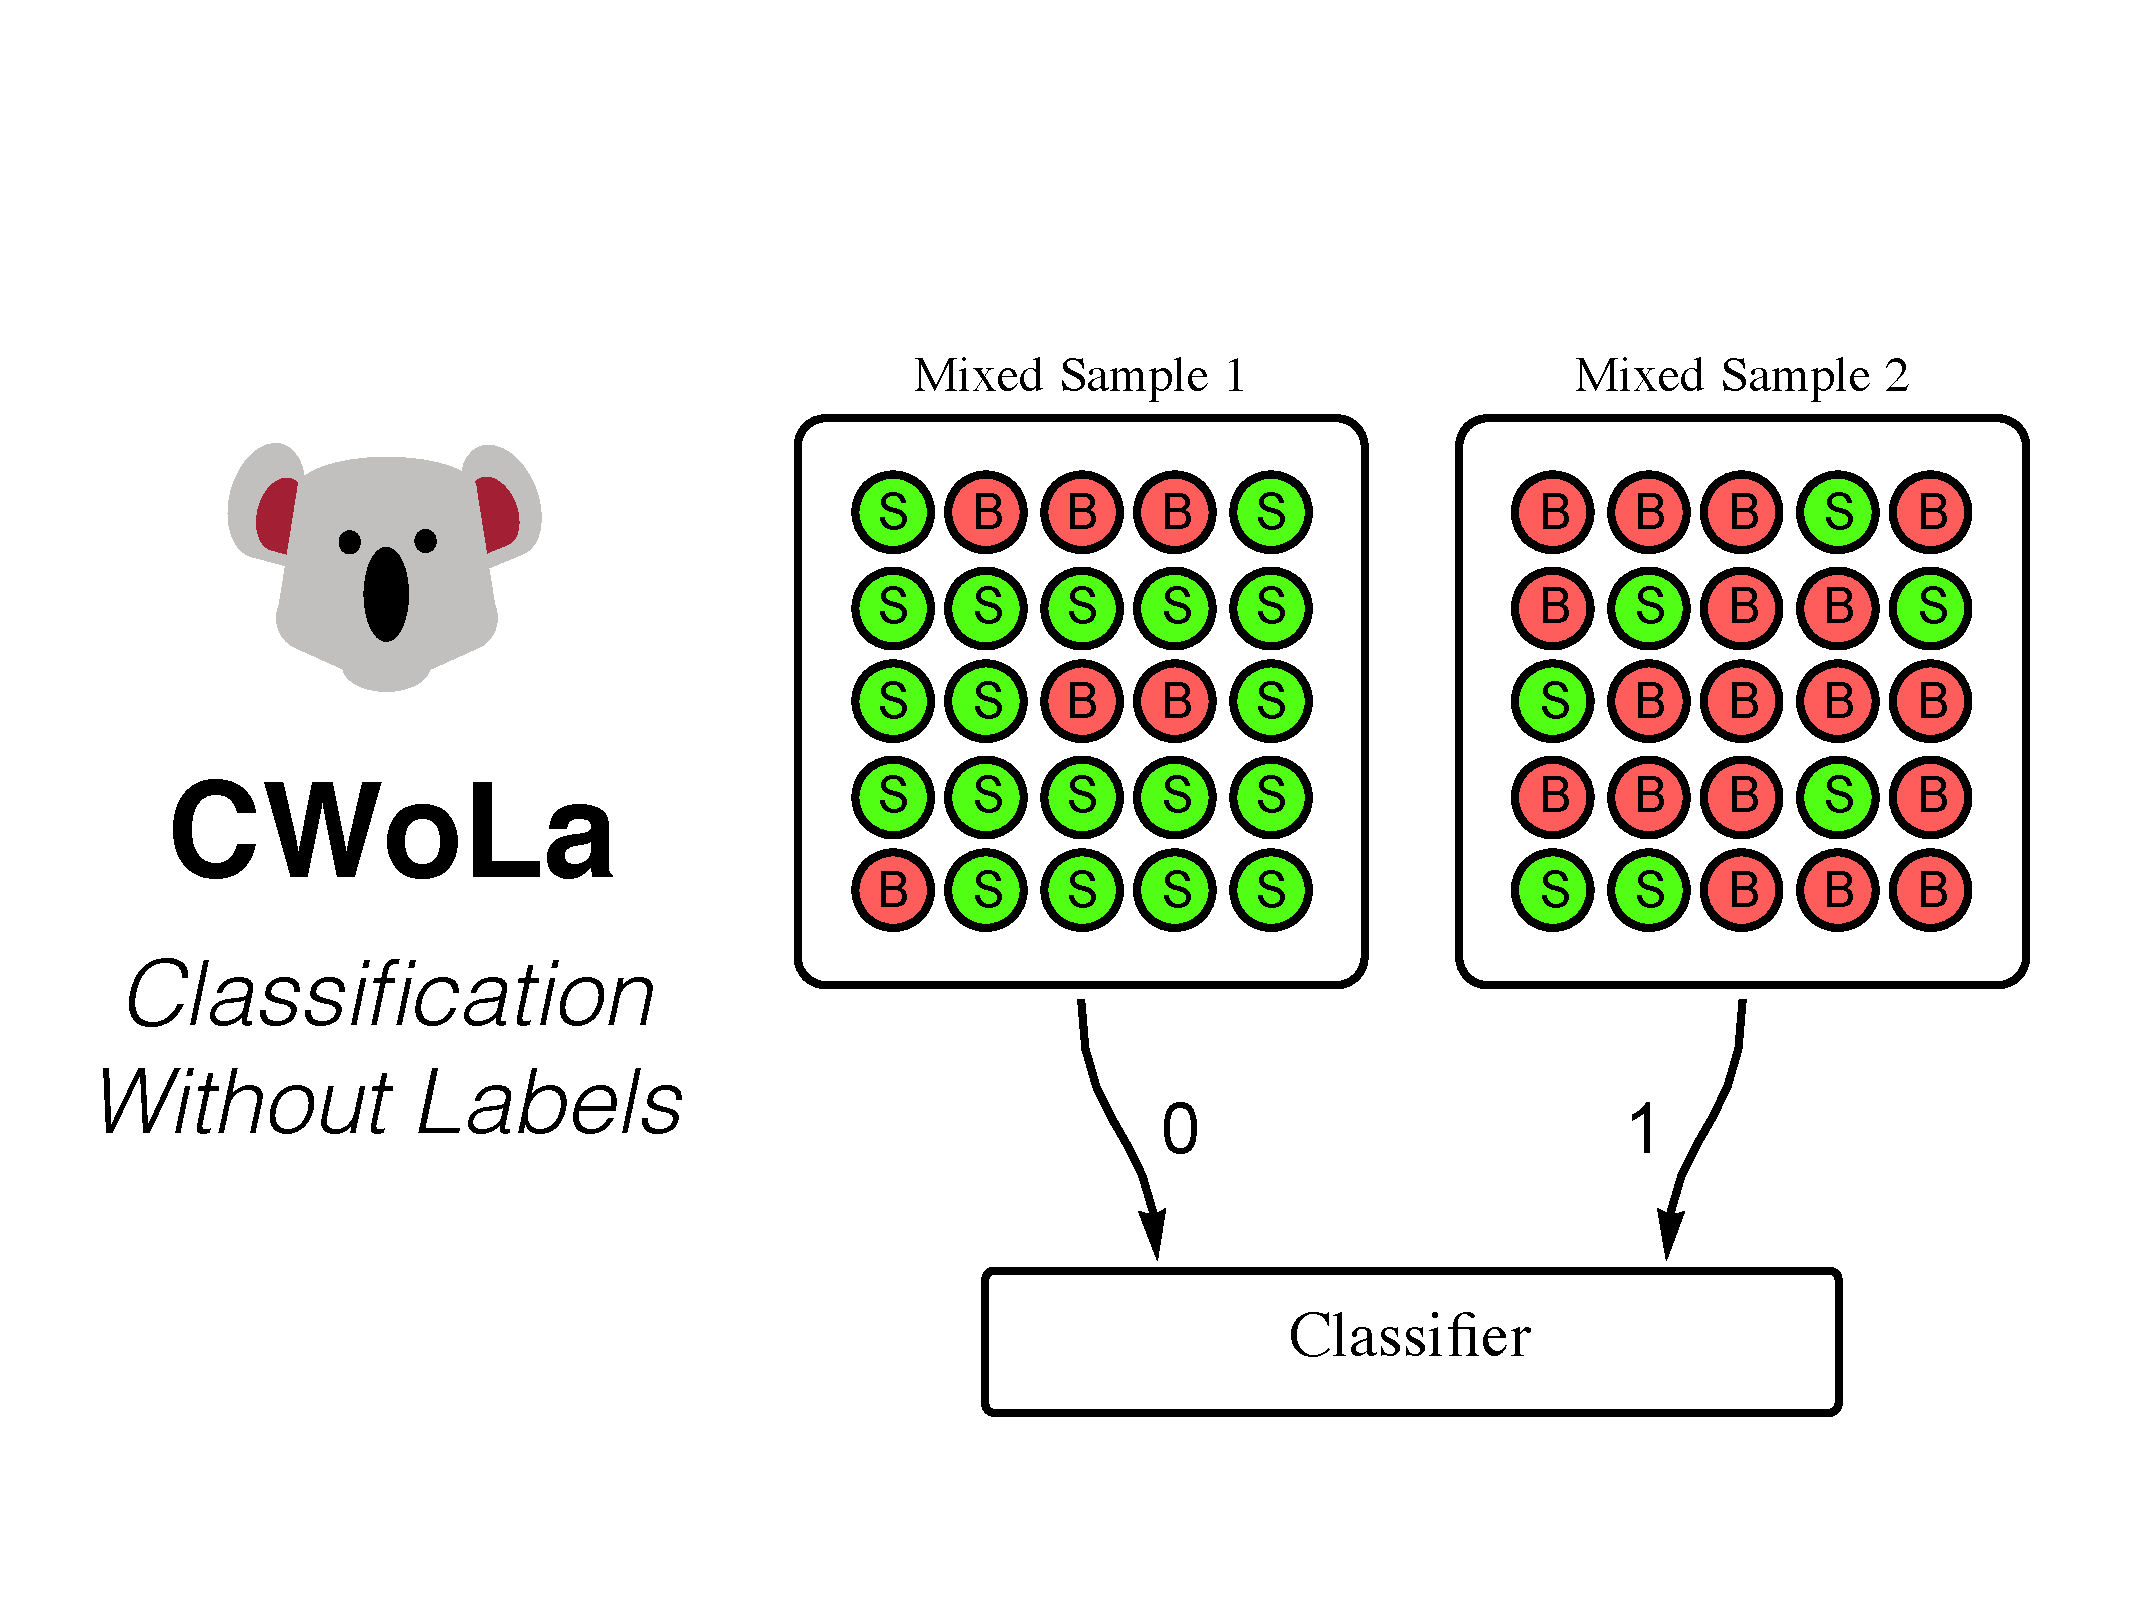
\includegraphics[width=0.6\textwidth]{figures_CWoLa/cwola.pdf}
\caption{In the setup of classification without labels, there are two mixed samples with an unknown composition of signal and background.  In the CWoLa approach, all events in the first of these two mixed samples is labeled 0 and all events in the second mixed sample are labeled 1.  A supervised classifier is then trained to distinguish between the 0's and 1's.  This same classifier is then used to distinguish signal from background.}
\label{fig:CWoLa:cwolasetup}
\end{figure}

As mentioned above, the second drawback of traditional supervised learning is that one needs a signal model.  The idea of `CWoLa hunting'~\cite{Collins:2018epr,Collins:2019jip} is to use the CWoLa training scheme to look for BSM physics without a particular signal model in mind.  The setup for the CWoLa-based search is shown schematically in Figure~\ref{fig:CWoLa:cwolahuntingsetup}.  There is one dimension where a potential signal is known to be localized (`resonant'), denoted $m_\text{res}$.  Two mixed samples are formed: one centered on the potential resonance and one formed on regions just to the left and right of the signal region.  These sideband regions should be as small as possible so that other properties of the events do not change significantly between the signal region and sideband region, but as large as possible to have sufficient training statistics.  Features (`y') that are approximately orthogonal (this statement is made more precise in Section~\ref{sec:CWoLa:Analysis:Overview}) are then used for the CWoLa training described above.  If there is signal in the signal region, then placing a threshold on the resulting neural network should enhance it over the background.  This process is then repeated for different partitions of signal and sideband to be sensitive to a broad spectrum of BSM masses.  One of the key aspects of the full technique is a nested cross-validation procedure in order to mitigate the look-elsewhere effect.  This is described in Section~\ref{sec:CWoLa:network}.

\begin{figure}
\centering
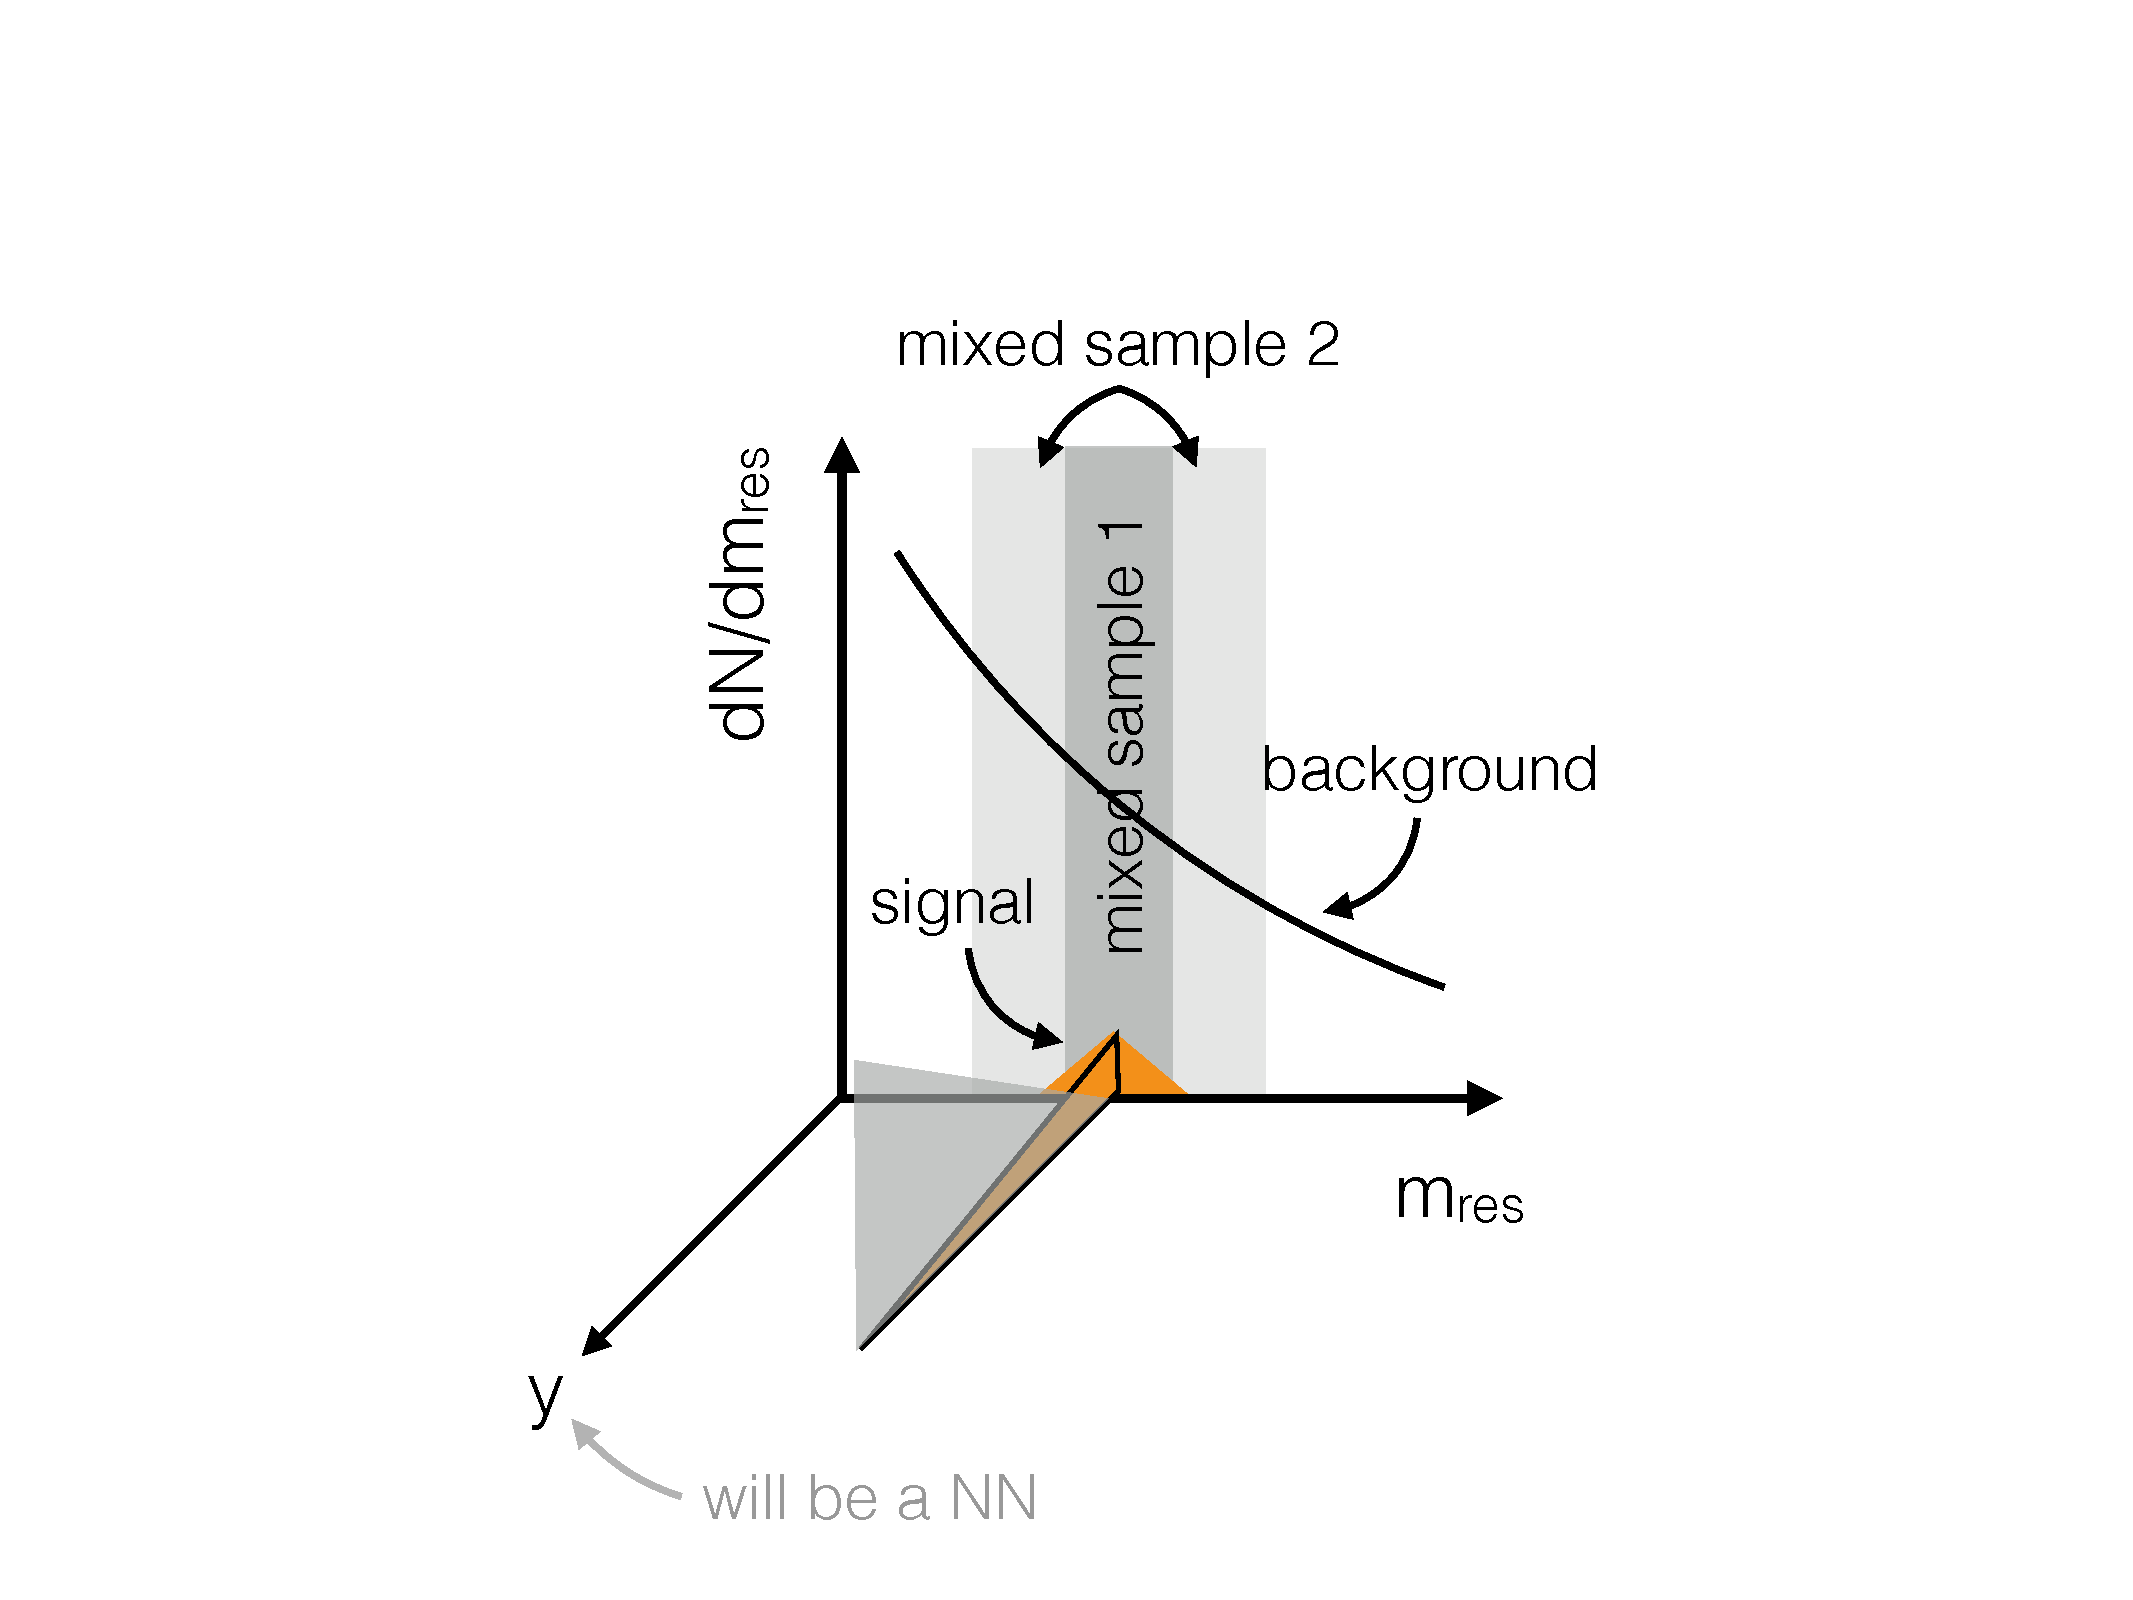
\includegraphics[width=0.5\textwidth]{figures_CWoLa/cwolahuntingsetup.pdf}
\caption{The setup for a search-based application of the CWoLa technique.  The other features $y$ can be used to train CWoLa.  The requirement is that $y$ is (nearly) independent of $m_\text{res}$.  Note that it is okay if there is some signal in the sidebands.}
\label{fig:CWoLa:cwolahuntingsetup}
\end{figure}

The next sections describes our analysis strategy, based on the above ideas ($m_\text{res}=m_{JJ}$), in detail.

%\clearpage

\subsection{Overview}
\label{sec:CWoLa:Analysis:Overview}
This analysis utilizes the concept of Classification Without Labels (CWoLa) described in Section~\ref{sec:CWoLa:schematic} in order to be sensitive to a broad class of non-SM models of the form $A\rightarrow BC$, with $A$ massive and on-shell, and the decay products of $B$ and $C$ reconstructed as large-$R$ jets in the ATLAS calorimeter.
In these models, the reconstructed dijet mass $m_{JJ}$ will show a peak near the mass of the $A$, with width determined by the dijet mass resolution.
There are two key assumptions that enable this analysis to be sensitive to these models.
\begin{enumerate}
  \item \textbf{(Assumption 1)} One or both of the jets reconstructed from the $B$ and $C$ decays have features, e.g. in their substructure, which differ from the background composition (i.e., non-resonant dijet events from QCD and other SM processes), so that these jets can be tagged in order to increase the signal to background ratio of the signal $m_{JJ}$ peak over the background shape. \label{ass1}
  \item \textbf{(Assumption 2)} After tagging on these features, the background $m_{JJ}$ remains smooth, so that a fit to the background $m_{JJ}$ spectrum does not indicate a potential discovery via a bump in the $m_{JJ}$ spectrum. \label{ass2}
\end{enumerate}
In particular, clearly one of the features that differs between the signal and the background composition is $m_{JJ}$ itself; if $m_{JJ}$ is used as a feature, or if jet features that allow reconstruction of $m_{JJ}$ are used, then Assumption~\ref{ass2} is violated, because after tagging on this feature the $m_{JJ}$ spectrum in the background will no longer be smooth.
Therefore some effort must be put into choosing features that will not violate Assumption~\ref{ass2}, and into validating that the assumption is not violated once the features are chosen.

Under these assumptions, the outline of the analysis is as follows.
\begin{enumerate}
  \item Select events in which at least two large-$R$ jets are reconstructed, and in these events form the dijet invariant mass, $m_{JJ}$, and record some relevant jet features $X$.
  \item Partition the $m_{JJ}$ spectrum into discrete, monotonically increasing bins.
  \item Label one of these bins the \textit{signal region}, and the bins on either side in $m_{JJ}$ space the \textit{sideband regions}.~\label{step3}
  \item Train a neural network (NN) to distinguish between the signal region and the sideband regions based on the chosen features $X$.
    There are three possibilities of what the network learns, based on where the true signal lies relative to the signal region.
    \begin{enumerate}
      \item If the signal mass peak happens to lie in the signal region, then the signal fraction in the signal region will be higher than in the sideband regions, and the network will learn that it can identify some events in the signal region by tagging the true signal; i.e., the network will learn how to tag signal events.
        This process is what is referred to as CWoLa.\label{case1}
      \item If the signal mass peak happens to lie in one of the sideband regions, then the signal fraction in the signal region will be lower than in the sideband regions, and the network will learn to identify some events in the sideband region by tagging the true signal; i.e., the network will learn how to anti-tag signal events.\label{case2}
      \item If the signal mass peak does not lie in the signal region or sideband regions, or if there is no signal at all, then the network will learn to distinguish between the background events in the signal and sideband regions based on the features $X$, as far as such correlations exist.\label{case3}
    \end{enumerate}
    Note that, in Cases~\ref{case1} and~\ref{case2}, the network is sensitive to both the difference in the distribution of the features $X$ between the signal and the background, and to the differences between the background in the signal region and the background in the sideband regions.
    In order to allow the network to focus on tagging the signal versus the background, the sideband regions are chosen to be adjacent to the signal region in kinematic space so that the difference in the features in the background between the signal and sideband regions is minimzed.
  \label{step4}
  \item Tag events by choosing events with high neural network output.
    In Case~\ref{case1}, the neural network is a signal tagger, so the signal-to-background ratio increases, in particular increasing the significance of the signal peak over the background $m_{JJ}$ shape. 
    In Case~\ref{case2}, the network anti-tags signal, and in Case~\ref{case3}, the network tags only differences in the background between signal and sideband regions; in either case, the signal-to-background ratio after tagging is small or zero.
  \item Fit to the $m_{JJ}$ shape after tagging.
    Because of Assumption~\ref{ass2}, the background spectrum is smooth after tagging.
    In Case~\ref{case1}, there will be a bump in the $m_{JJ}$ spectrum in the signal region due to the presence of signal, allowing the potential of a discovery of this signal.
    In Cases~\ref{case2} and~\ref{case3}, there will be little to no signal, so there will be no bump in the $m_{JJ}$ spectrum, and the spectrum fit will not indicate the discovery of a signal.
    \label{step6}
  \item Repeat Steps~\ref{step3}-\ref{step6} with each possible signal region bin.
    If there is any true signal, then the signal will lie in one of the signal region bins, and Case~\ref{case1} will be true in that bin, allowing discovery of this signal.
    If there is no true signal, then in each signal region bin Case~\ref{case3} will be true, thus indicating no discovery over the whole $m_{JJ}$ range.
\end{enumerate}
Since there is a difference in the observed outcomes between the case where there is presence of signal and when there is no signal, limits can be set on specific signal models based on what would have been observed if those signals were present.

Since the network learns what features distinguish the signal from the background automatically, this analysis is sensitive to a wide range of possible signal distributions of these features, and thus the analysis can be sensitive to a wide range of signal models without paying the price of a look-elsewhere effect that a dedicated search for each one of these signal models would entail.

Furthermore, since the network learns the features that distinguish the signal from the background directly from data, the tagger does not need to be calibrated to account for differences between simulation and background; this removes a source of uncertainty relative to a dedicated search with a tagger trained to distinguish between signal and background in simulation.

\subsection{Features}
\label{sec:CWoLa:features}
In Analysis Step~\ref{step4}, some features $X$ are designated which, as per Assumption~\ref{ass1}, can be used to distinguish signals from the background.
In this analysis, only the masses of the two jets, $X = \{m_1,m_2\}$, are used as features.

The distributions of $m_1$ and $m_2$ in the background using the nominal simulation are plotted in various $m_{JJ}$ regions in Figure~\ref{fig:CWoLa:bkg_m1_m2}.
The distributions of $m_1$ and $m_2$ in a variety of signal models are plotted in the $m_{JJ}$ region which is most efficient on that signal in Figure~\ref{fig:CWoLa:sig_m1_m2}.
It can be seen that the masses of the signal objects, $m_B$ and $m_C$, are well-reconstructed as $m_1$ and $m_2$.

\begin{figure}[htbp]
  \centering 
  \subfloat[]{\includegraphics[width=0.3\textwidth]{figures_CWoLa/{jet1_m_jet2_m_sigR0_4.10.19}.png}}
  \subfloat[]{\includegraphics[width=0.3\textwidth]{figures_CWoLa/{jet1_m_jet2_m_sigR1_4.10.19}.png}}
  \subfloat[]{\includegraphics[width=0.3\textwidth]{figures_CWoLa/{jet1_m_jet2_m_sigR2_4.10.19}.png}}\\
  \subfloat[]{\includegraphics[width=0.3\textwidth]{figures_CWoLa/{jet1_m_jet2_m_sigR3_4.10.19}.png}}
  \subfloat[]{\includegraphics[width=0.3\textwidth]{figures_CWoLa/{jet1_m_jet2_m_sigR4_4.10.19}.png}}
  \subfloat[]{\includegraphics[width=0.3\textwidth]{figures_CWoLa/{jet1_m_jet2_m_sigR5_4.10.19}.png}}\\
  \subfloat[]{\includegraphics[width=0.3\textwidth]{figures_CWoLa/{jet1_m_jet2_m_sigR6_4.10.19}.png}}
  \subfloat[]{\includegraphics[width=0.3\textwidth]{figures_CWoLa/{jet1_m_jet2_m_sigR7_4.10.19}.png}}
  \subfloat[]{\includegraphics[width=0.3\textwidth]{figures_CWoLa/{jet1_m_jet2_m_sigR8_4.10.19}.png}}\\
  \subfloat[]{\includegraphics[width=0.3\textwidth]{figures_CWoLa/{jet1_m_jet2_m_sigR9_4.10.19}.png}}
  %\subfloat[]{\includegraphics[width=0.3\textwidth]{figures_CWoLa/{jet1_m_jet2_m_sigR10_4.10.19}.png}}
  \caption{Distribution of $m_1$ and $m_2$ in the background in $m_{JJ}$ regions (a) 0; (b) 1; (c) 2; (d) 3; (e) 4; (f) 5; (g) 6; (h) 7; (i) 8; (j) 9; (k) 10.  These bins are described in Section~\ref{sec:CWoLa:binning} and cover 1.1 TeV up to 8.17 TeV.}
\label{fig:CWoLa:bkg_m1_m2}
\end{figure}

\begin{figure}[htbp]
  \centering 
  \subfloat[]{\includegraphics[width=0.3\textwidth]{figures_CWoLa/{jet1_m_jet2_m_Wprime_WZqqqq_M3000_m80_m80_1.14.20}.png}}
  \subfloat[]{\includegraphics[width=0.3\textwidth]{figures_CWoLa/{jet1_m_jet2_m_Wprime_WZqqqq_M3000_m80_m200_1.14.20}.png}}
  \subfloat[]{\includegraphics[width=0.3\textwidth]{figures_CWoLa/{jet1_m_jet2_m_Wprime_WZqqqq_M3000_m80_m400_1.14.20}.png}}\\
  \subfloat[]{\includegraphics[width=0.3\textwidth]{figures_CWoLa/{jet1_m_jet2_m_Wprime_WZqqqq_M3000_m200_m200_1.14.20}.png}}
  \subfloat[]{\includegraphics[width=0.3\textwidth]{figures_CWoLa/{jet1_m_jet2_m_Wprime_WZqqqq_M3000_m200_m400_1.14.20}.png}}
  \subfloat[]{\includegraphics[width=0.3\textwidth]{figures_CWoLa/{jet1_m_jet2_m_Wprime_WZqqqq_M3000_m400_m400_1.14.20}.png}}\\
  \subfloat[]{\includegraphics[width=0.3\textwidth]{figures_CWoLa/{jet1_m_jet2_m_Wprime_WZqqqq_M5000_m80_m80_1.14.20}.png}}
  \subfloat[]{\includegraphics[width=0.3\textwidth]{figures_CWoLa/{jet1_m_jet2_m_Wprime_WZqqqq_M5000_m80_m200_1.14.20}.png}}
  \subfloat[]{\includegraphics[width=0.3\textwidth]{figures_CWoLa/{jet1_m_jet2_m_Wprime_WZqqqq_M5000_m80_m400_1.14.20}.png}}\\
  \subfloat[]{\includegraphics[width=0.3\textwidth]{figures_CWoLa/{jet1_m_jet2_m_Wprime_WZqqqq_M5000_m200_m200_1.14.20}.png}}
  \subfloat[]{\includegraphics[width=0.3\textwidth]{figures_CWoLa/{jet1_m_jet2_m_Wprime_WZqqqq_M5000_m200_m400_1.14.20}.png}}
  \subfloat[]{\includegraphics[width=0.3\textwidth]{figures_CWoLa/{jet1_m_jet2_m_Wprime_WZqqqq_M5000_m400_m400_1.14.20}.png}}\\
  \caption{Distribution of $m_1$ and $m_2$ in for a signal model with
    (a) ($m_A,m_B,m_C=3000,80,80$ GeV);
    (b) ($m_A,m_B,m_C=3000,200,80$ GeV);
    (c) ($m_A,m_B,m_C=3000,400,80$ GeV);
    (d) ($m_A,m_B,m_C=3000,200,200$ GeV);
    (e) ($m_A,m_B,m_C=3000,400,20$ GeV);
    (f) ($m_A,m_B,m_C=3000,400,400$ GeV).
    (g) ($m_A,m_B,m_C=5000,80,80$ GeV);
    (h) ($m_A,m_B,m_C=5000,200,80$ GeV);
    (i) ($m_A,m_B,m_C=5000,400,80$ GeV);
    (j) ($m_A,m_B,m_C=5000,200,200$ GeV);
    (k) ($m_A,m_B,m_C=5000,400,20$ GeV);
    (l) ($m_A,m_B,m_C=5000,400,400$ GeV).
  }
\label{fig:CWoLa:sig_m1_m2}
\end{figure}

Since $m_1$ and $m_2$ peak around the values of $m_B$ and $m_C$ in the signal, while they have smoothly falling spectra in the background, these features satisfy Assumption~\ref{ass1}, and therefore can be used for the training.

\subsubsection{Mass Decorrelation}
\label{sec:CWoLa:decorrelation}
In Figure~\ref{fig:CWoLa:bkg_m1_m2}, it can be seen that there are true physical differences in the features in the background between a given signal region and sideband regions (as chosen in Analysis Step~\ref{step3}); in particular, the distribution gets more populated at higher $m_1$,$m_2$ as $m_{JJ}$ increases.
This therefore requires some modification of these features in order to satisfy Assumption~\ref{ass2}.

The idea is to scale the 1-dimensional marginal distribution of the jet mass $m$ (combining both $m_1$ and $m_2$ across all events) in the sideband regions to the signal region.
This is accomplished by constructing the empirical cumulative distribution function (ECDF) in each region $s$:
\begin{align}
  \Phi_s(m) = \frac{1}{n_s} \sum_{j=1}^{n_s} \mathbbm{1}(m_j\le m)
\end{align}
Where $n_s$ is the number of jets in $m_{JJ}$ region $s$, $\mathbbm{1}$ is the indicator function, and $j$ goes over all jets (leading and subleading) in region $s$.\footnote{Actually, $\Phi_s(m)$ is evaluated at all values of $m$ that exist in the $m_{JJ}$ region, and then is linearly interpolated for intermediate values.}
Note that the distribution of $\Phi_s(m)$ over all jets in $m_{JJ}$ region $s$ is by definition uniform; and that the distribution of $\Phi^{-1}_s(x)$ is exactly the distribution of $m$ in $m_{JJ}$ region $s$, if $x$ follows a uniform distribution.
The ECDF is a good approximation of the true CDF in regions where there are a sufficient number of samples.
This motivates the choice to place a maximum cut on the jet mass at $500 \GeV$, in order to restrict to the region in which the CDF can be approximated well.

Then, for a given signal segion $s$, the masses of all jets in the sideband segions $s-1$ and $s+1$ are rescaled to the signal segion:
\begin{align}
  \begin{cases}
    m \rightarrow \Phi^{-1}_s\left(\Phi_{s-1}\left(m\right)\right) & m \in \text{region } s-1 \\
    m \rightarrow \Phi^{-1}_s\left(\Phi_{s+1}\left(m\right)\right) & m \in \text{region } s+1
  \end{cases}
\end{align}
This insures that the 1-dimensional distributions of $m$ in the sideband regions are exactly the same, by construction, as in the signal region.
Note that, if there is a signal present in the signal region, that the scaling will be slightly biased by the presence of this signal, depending on the signal fraction in that region.
This scaling is demonstrated for an example signal and sideband regions in Figure~\ref{fig:CWoLa:m_scaling}, including an example with an injected signal.
\begin{figure}[t!]
    \centering
    \subfloat[]{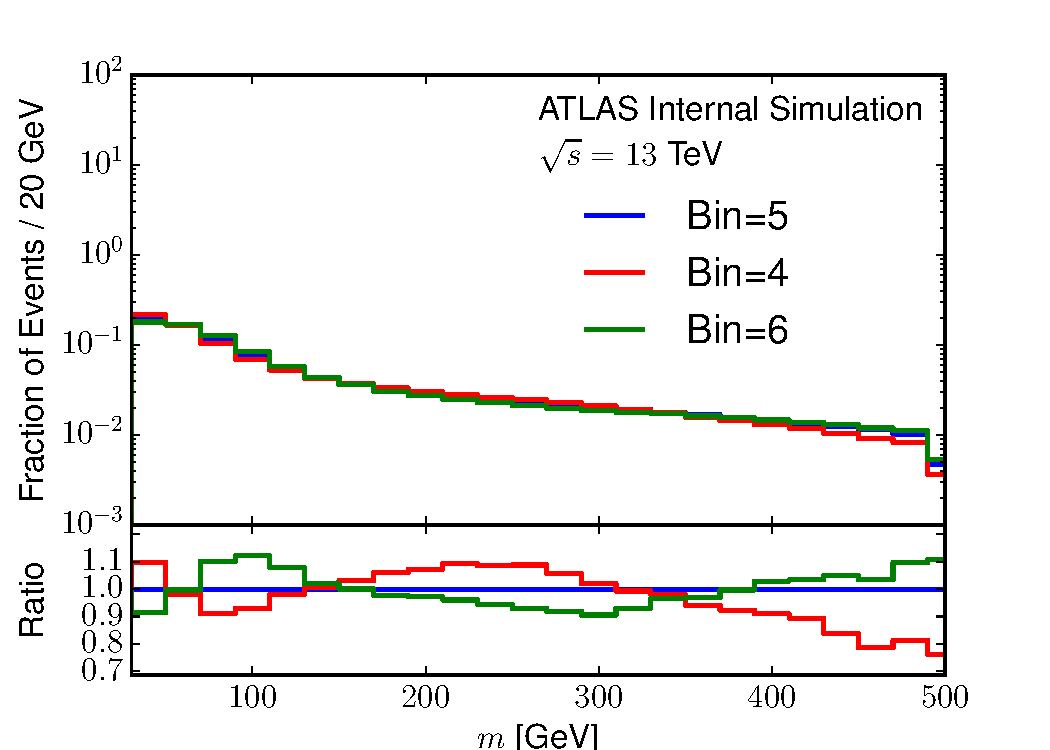
\includegraphics[width=0.45\textwidth]{{figures_CWoLa/jet_m_log_mjjbins_sigR5_4.10.19}.pdf}}
    \subfloat[]{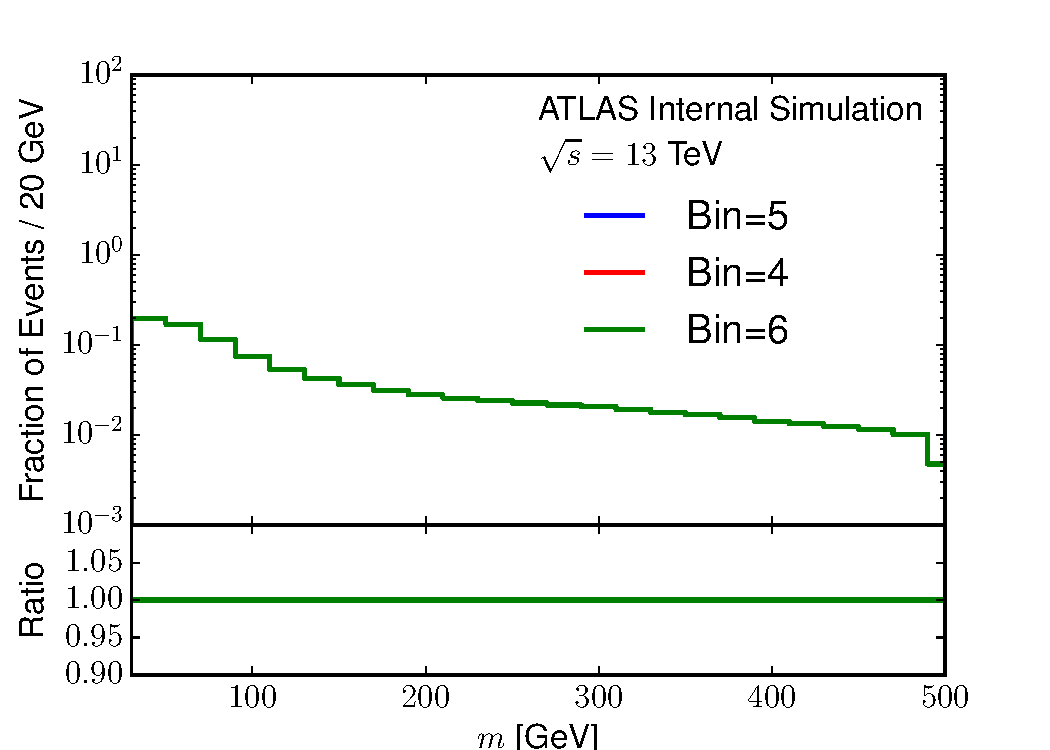
\includegraphics[width=0.45\textwidth]{{figures_CWoLa/jet_m_scaled_log_mjjbins_sigR5_4.10.19}.pdf}}\\
    \subfloat[]{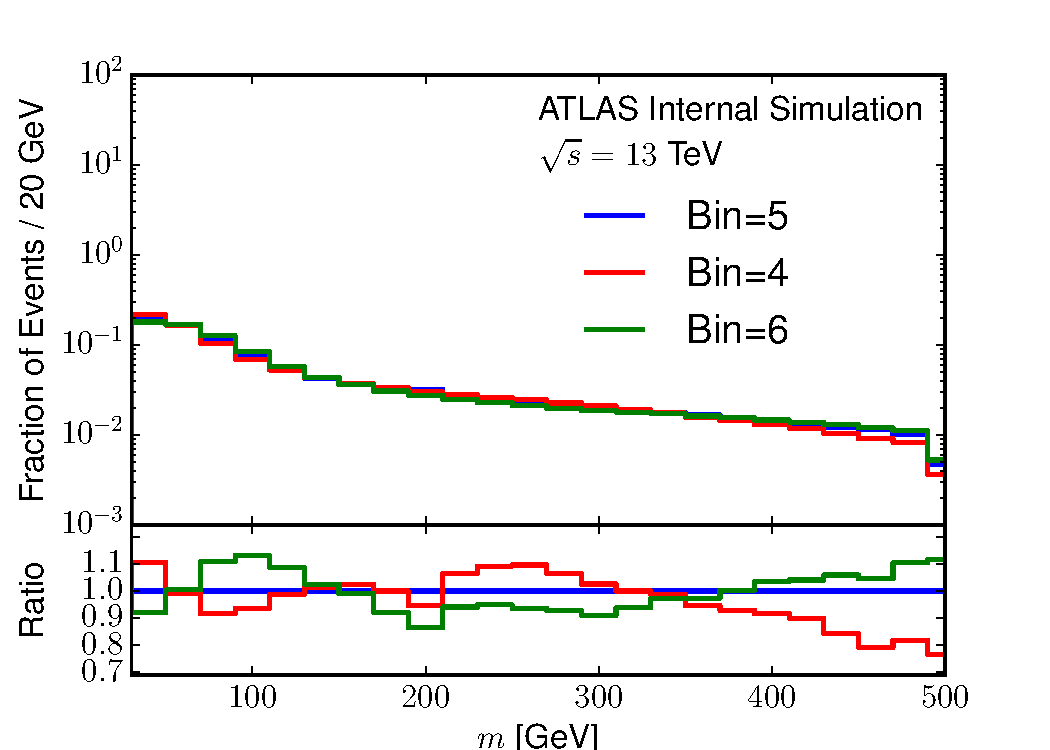
\includegraphics[width=0.45\textwidth]{{figures_CWoLa/jet_m_log_mjjbins_sigR5_Wprime_WZqqqq_M3000_m200_m200_nS2000_4.10.19}.pdf}}
    \subfloat[]{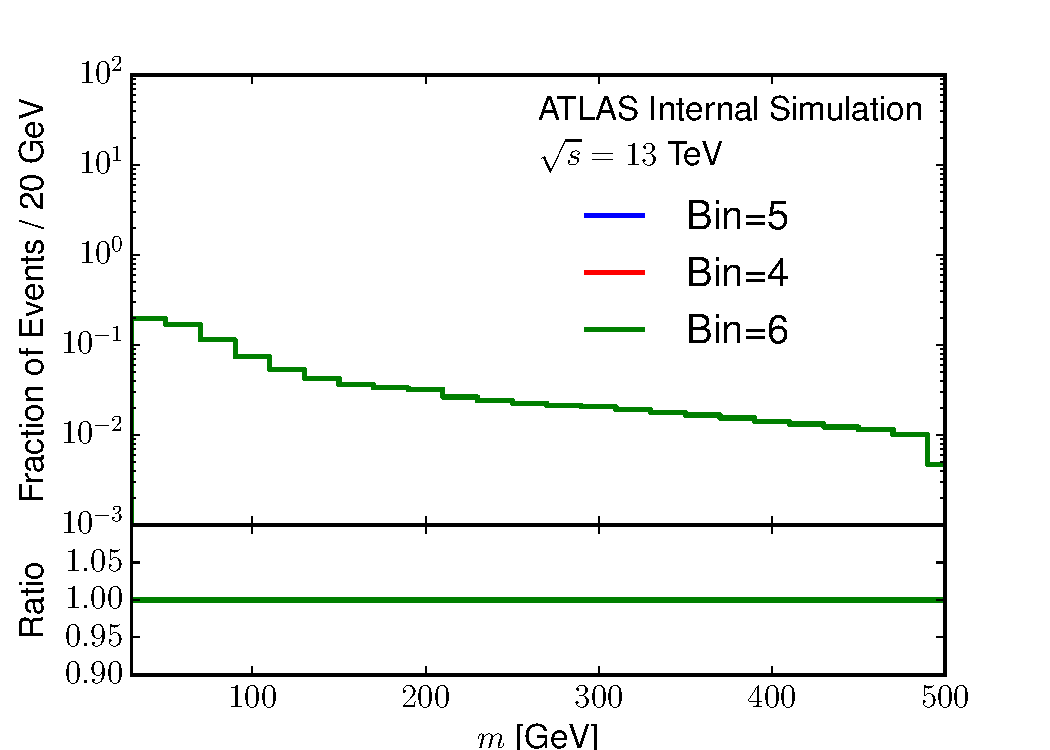
\includegraphics[width=0.45\textwidth]{{figures_CWoLa/jet_m_scaled_log_mjjbins_sigR5_Wprime_WZqqqq_M3000_m200_m200_nS2000_4.10.19}.pdf}}
    \caption{The distributions of $m$, comparing between signal region $s=5$ and sideband regions $s-1=4$ and $s+1=6$. (a) Before any scaling. (b) After scaling via the empirical cumulative distribution function. (c) Including an injected signal sample with $m_A,m_B,m_C=3000,200,200$ GeV, which lies mostly in signal segion 5, and with $\frac{S}{\sqrt{B}}\sim 2$ in that region. (d) After scaling, with the presence of the signal sample.   Bin 4 covers 2.28 $<m_{JJ}<2.74$ TeV, bin 5 covers 2.74 $<m_{JJ}<3.28$ TeV and bin 6 covers 3.28 $<m_{JJ}<3.94$ TeV.}
    \label{fig:CWoLa:m_scaling}
\end{figure}

After the 1-dimensional scaling the only differences that can exist are in the 2-dimensional distribution $m_1$ and $m_2$, which can arise due to differences in the correlation between $m_1$ and $m_2$ between the regions.
It is expected that in the background these differences are small, and this is supported by examining the distributions of $m_1$ and $m_2$ in simulation, as can be seen in Figure~\ref{fig:CWoLa:LR2D}.

The presence of a signal in one of the regions is exactly such a difference that can exist in the correlations between $m_1$ and $m_2$.
Therefore, even though the scaling can be biased by the presence of a signal in the signal region, it is expected that there will still exist differences in the 2-dimensional distribution between the signal and sideband regions, as can be seen in Figure~\ref{fig:CWoLa:LR2D}.
\begin{figure}[t!]
    \centering
    \subfloat[]{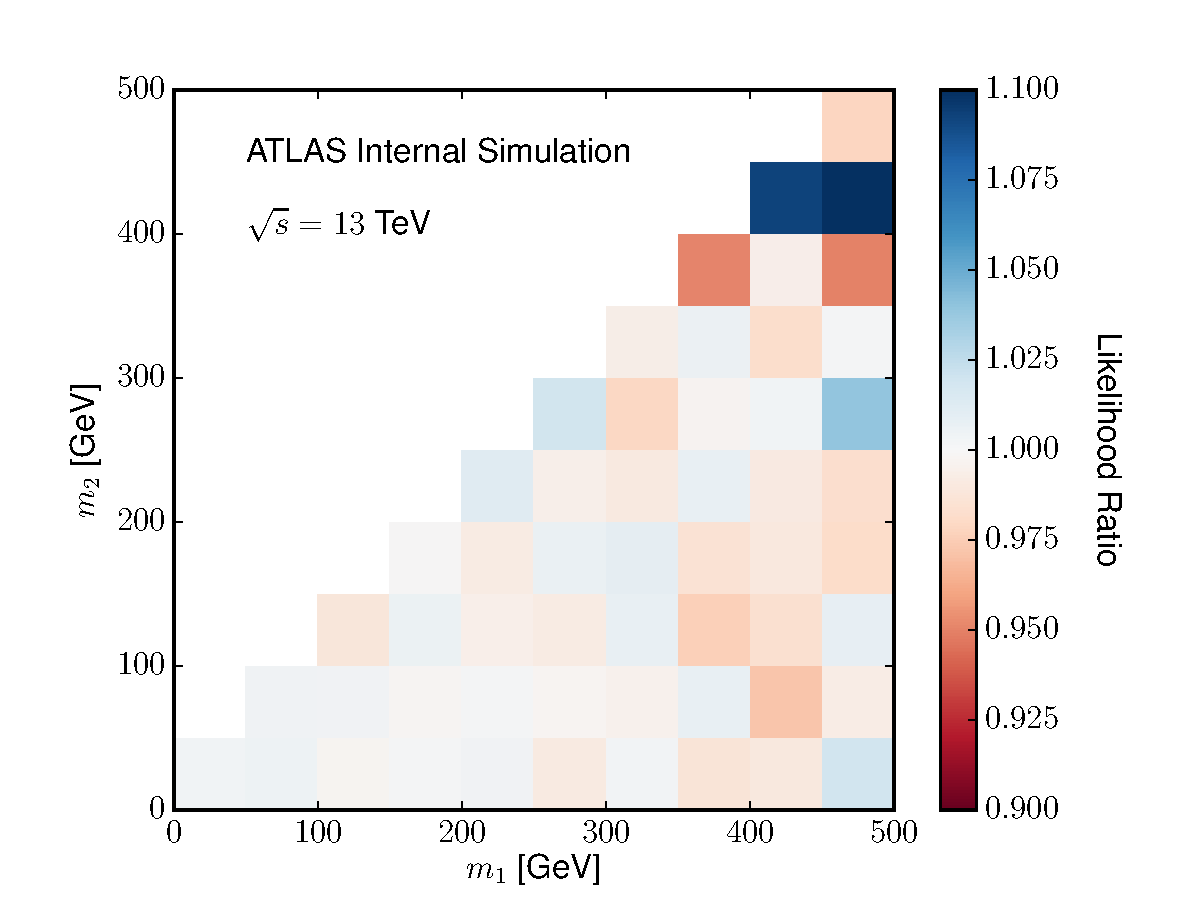
\includegraphics[width=0.3\textwidth]{{figures_CWoLa/jet_m1_m2_scaled_ratiolow_sigR5_scaleall_4.10.19}.pdf}}
    \subfloat[]{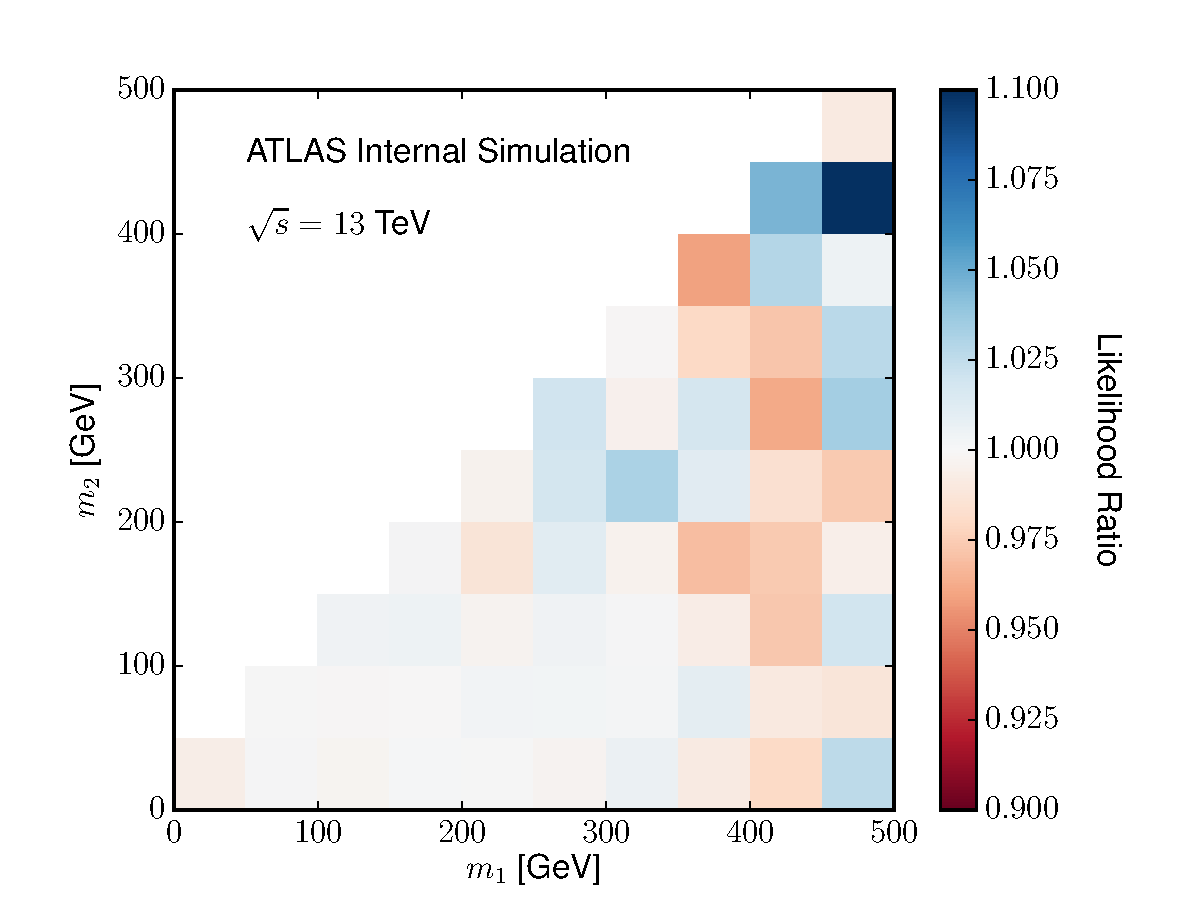
\includegraphics[width=0.3\textwidth]{{figures_CWoLa/jet_m1_m2_scaled_ratiohigh_sigR5_scaleall_4.10.19}.pdf}}
    \subfloat[]{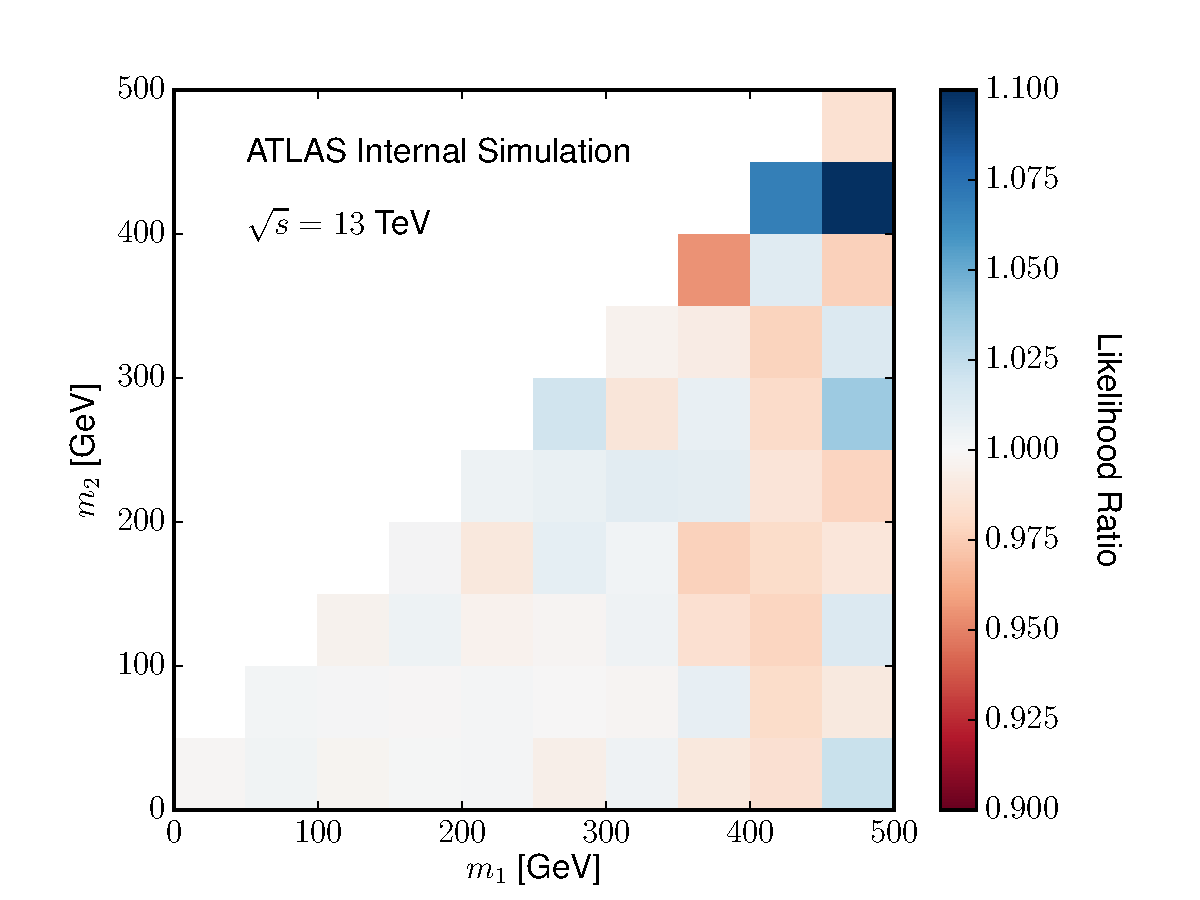
\includegraphics[width=0.3\textwidth]{{figures_CWoLa/jet_m1_m2_scaled_ratio_sigR5_scaleall_4.10.19}.pdf}}\\
    \subfloat[]{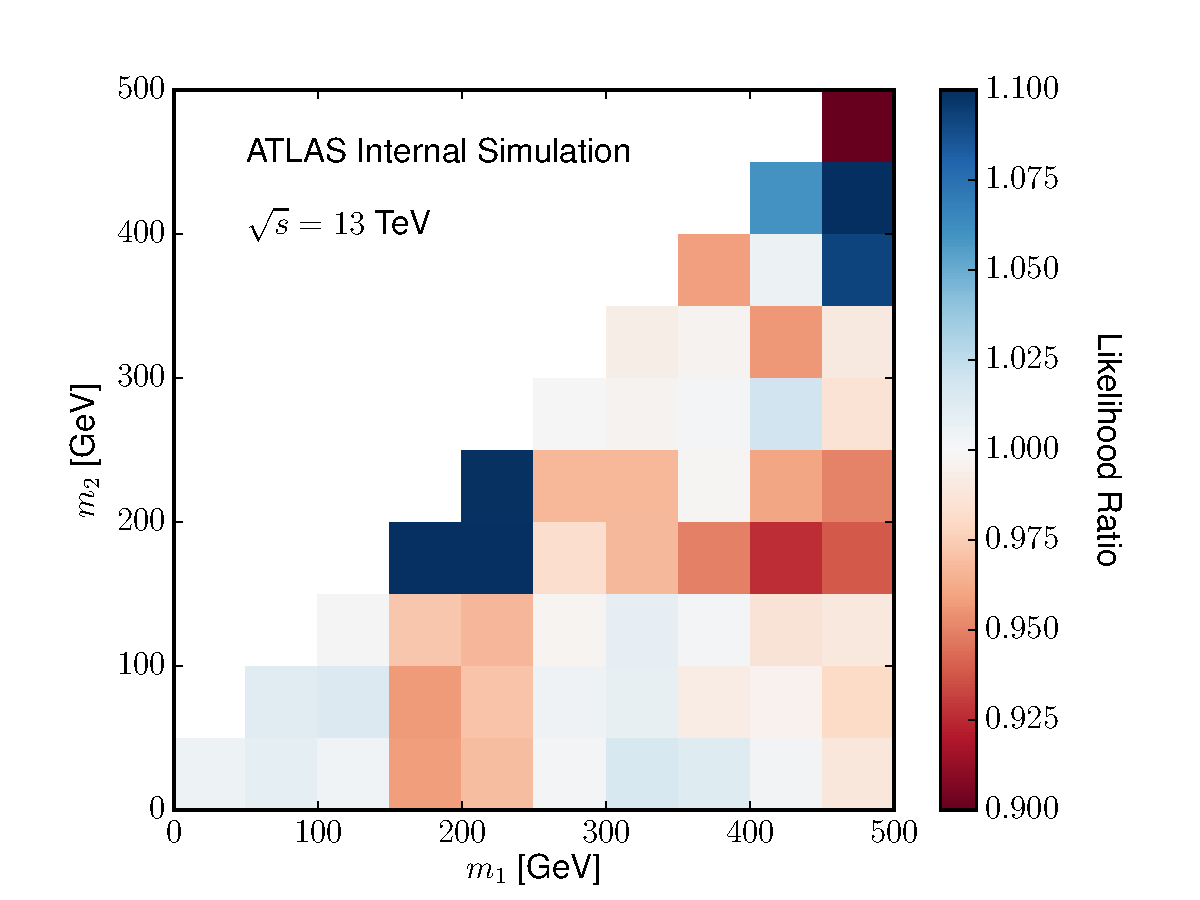
\includegraphics[width=0.3\textwidth]{{figures_CWoLa/jet_m1_m2_scaled_ratiolow_sigR5_Wprime_WZqqqq_M3000_m200_m200_nS2000_4.10.19}.pdf}}
    \subfloat[]{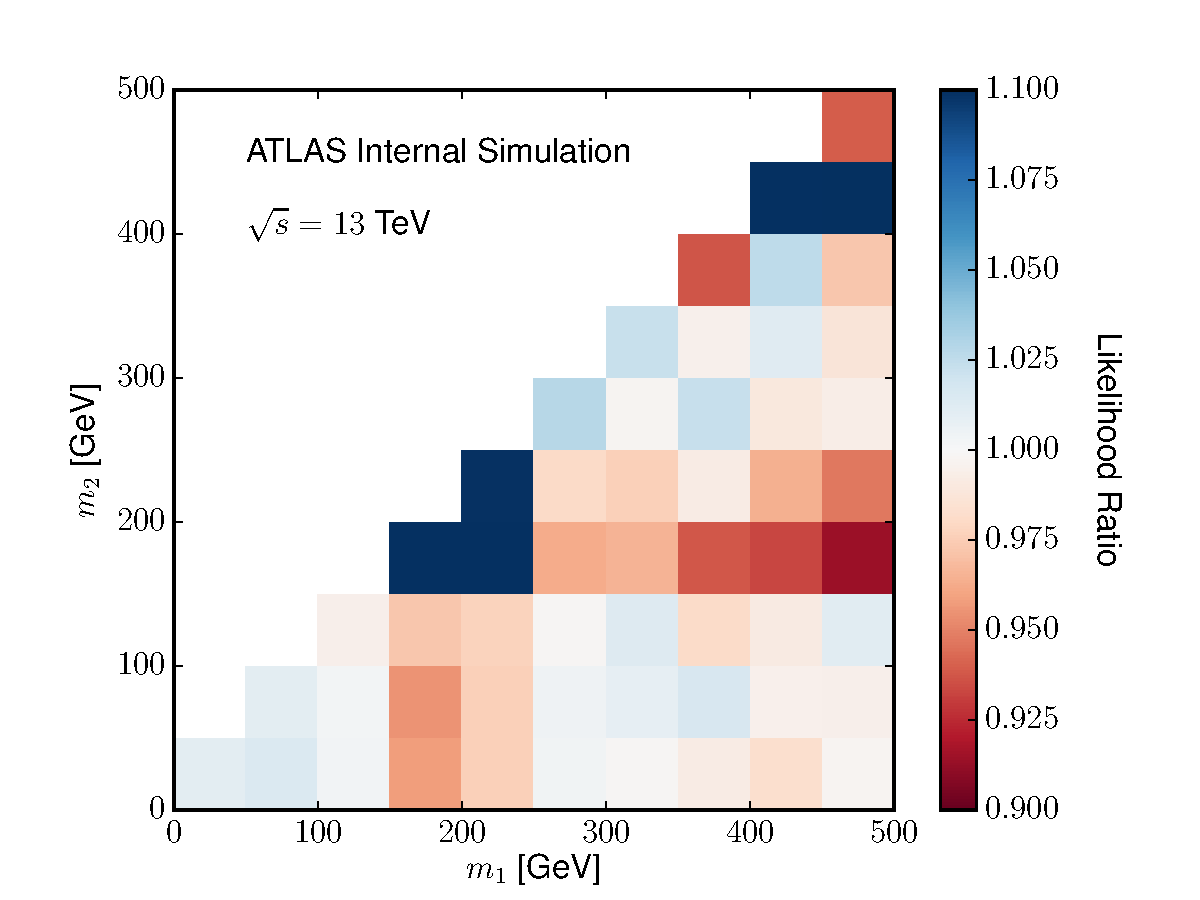
\includegraphics[width=0.3\textwidth]{{figures_CWoLa/jet_m1_m2_scaled_ratiohigh_sigR5_Wprime_WZqqqq_M3000_m200_m200_nS2000_4.10.19}.pdf}}
    \subfloat[]{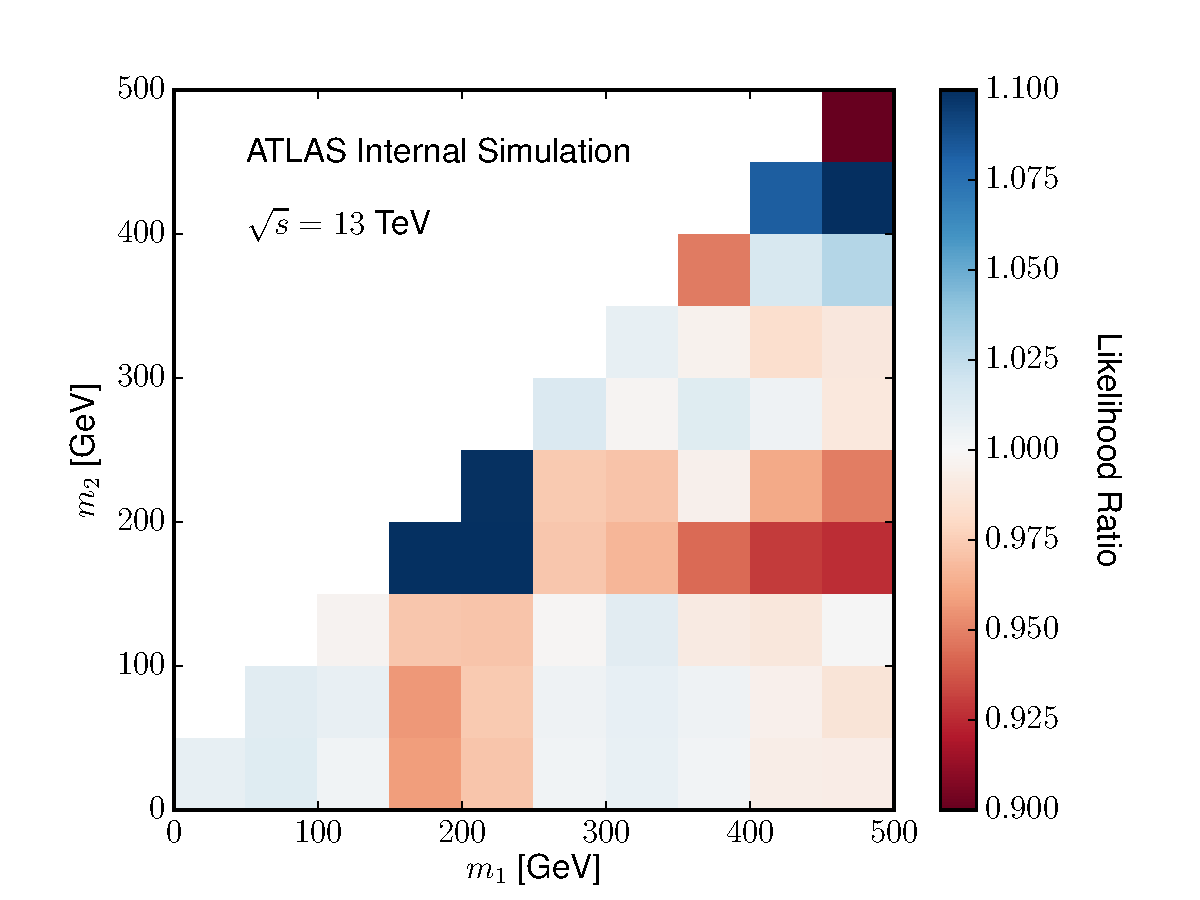
\includegraphics[width=0.3\textwidth]{{figures_CWoLa/jet_m1_m2_scaled_ratio_sigR5_Wprime_WZqqqq_M3000_m200_m200_nS2000_4.10.19}.pdf}}
    \caption{The 2-dimensional likelihood ratio in $m_1$ and $m_2$ after scaling, comparing between signal region $s=5$ and (a) sideband region $s-1=4$; (b) sideband region $s+1=6$; and (c) combining sideband regions $4$ and $6$, as described in Section~\ref{sec:CWoLa:network}.
    (d,e,f) Including an injected signal sample with $m_A,m_B,m_C=3000,200,200$ GeV, which lies mostly in signal region 5, and with $\frac{S}{\sqrt{B}}\sim 2$ in that region. Bin 4 covers 2.28 $<m_{JJ}<2.74$ TeV, bin 5 covers 2.74 $<m_{JJ}<3.28$ TeV and bin 6 covers 3.28 $<m_{JJ}<3.94$ TeV.}
    \label{fig:CWoLa:LR2D}
\end{figure}

\subsection{Neural Network Architecture}
\label{sec:CWoLa:network}
The network which determines the final score for each event, indicating more or less signal-like, is derived in multiple stages.
These stages are intended to maximize the sensitivity to new potential signals, while remaining robust to statistical fluctuations and true correlations in the background.

In Analysis Step~\ref{step3} (Section~\ref{sec:CWoLa:Analysis:Overview}), some signal bin $s$ is designated. The process below can then be considered an enumeration of the steps in Analysis Step~\ref{step4} (Section~\ref{sec:CWoLa:Analysis:Overview}).  See also Figure~\ref{fig:CWoLa:flowchart} for an overview. 

\begin{enumerate}
  \item Designate the sideband regions $s+1$ (the ``upper" sideband) and $s-1$ (the ``lower" sideband). 
  \label{NNstep2}
  \item All events in the entire dataset are separated randomly into 5 equally-sized \textit{cross-validation} sets $i \in [0-4]$.
  \label{NNstep1}
  \item Designate one of the cross-validation sets $i_t$ as the \textit{test set}.
  \label{NNstep3}
  \item Designate a different cross-validation set $i_v \ne i_t$ as the \textit{validation set}. The remaining 3 cross-validation sets are designated as the \textit{training set}.
  \label{NNstep5}
  \item A network is trained using just the training set, with features $X = \{m_1,m_2\}$, rescaled as described in Section~\ref{sec:CWoLa:decorrelation}. The events are labeled with $Y \in [0,1]$, with $1$ indicating an event in the signal region, and $0$ indicating an event in the sidebands. The events in each of the sideband regions are weighted uniformly in the training so that the sum of weights in each of the sideband regions is equal.

  The network is a Sequential Neural Network with 4 hidden layers of size 64,32,8,1, and activation functions \texttt{ReLu},\texttt{ReLu},\texttt{ReLu},sigmoid, respectively, as implemented in \texttt{Keras}~\cite{chollet2015keras}.
  The loss used is the binary cross-entropy, and the training loss is minimized using the \texttt{Adam}~\cite{kingma2014adam} optimizer.
  The loss is evaluated on the validation set.
  
  Total number of epochs is 1000, with an early stopping with patience of 100 on the validation loss. The batch size is 1\% of the total.

  
  \label{NNstep6}
  \item Repeat Step~\ref{NNstep6} with 3 different random initial configurations of the neural network weights, and choose the network with the lowest validation loss. The other 2 networks are discarded.
  \label{NNstep7}

  Finally, this network is evaluated on the test set, and only the scores on the test set are recorded.

  \textbf{Scaling}
  \phantomsection
  \label{NNstep7scaling}

  The score from the neural network output is scaled monotonically as a quantile between 0 and 1 on the events in the signal region test set (note that the scores for all events in the test set are recorded, not just those in the signal region).
  That is to say, after the scaling, an event with a score of $0 \le \epsilon \le 1$ received a higher score from the neural network than exactly a fraction $\epsilon$ of the events in the signal region test set.
  The scaling is done in this way so that different networks can later be combined by averaging their scores; since the network output score is standardized, this averaging is meaningful.
  \item Repeat Steps~\ref{NNstep5}-\ref{NNstep7} by varying $i_v$ to each of the remaining cross-validation sets in turn, keeping the test set $i_t$ fixed.
    I.e., there are 4 different validation set choices for the given test set, and these steps are repeated for each one, resulting in 4 different networks.
    The scores from these 4 networks are then averaged, and the average score is further rescaled as described in Step~\ref{NNstep7scaling}.
  \label{NNstep8}
  \item Repeat Steps~\ref{NNstep3}-\ref{NNstep8} by varying the chosen test set $i_t$, for a total of 5 networks.
  The total sample is then combined together; since the score from each network is scaled to be an efficiency on its respective test set, and the test sets are equally sized, the score for each event remains an efficiency over the entire dataset.
  \label{NNstep9}
\end{enumerate}

Ultimately, there are $3\times4\times5 = 60$ neural networks trained for each signal region $s$. A flowchart of the process described above is given in Figure~\ref{fig:CWoLa:flowchart}, and the neural network outputs are shown at each step in the process for a sample with injected signal.

The events are separated into training, validation, and test sets as described above in order to reduce the effect of statistical fluctuations in the training.
Since the validation set is statistically independent from the training set, choosing the network with the lowest validation loss, as described in Step~\ref{NNstep7}, insures that the network which learns true correlations the best is chosen.
Since the test set is statistically independent from both the training and validation sets, the network cannot do artificially better by being biased by statistical fluctuations in the training or validation set.

The choice to train 4 different networks with each non-test set chosen to be a validation set in succession, as described in Step~\ref{NNstep8}, is again intended to reduce the sensitivity to statistical fluctuations in the training sets, since for each validation set the training set is (somewhat, but not entirely) different.
The averaging over the validation sets can be seen when going from the first column of Figure~\ref{fig:CWoLa:flowchart} to the second column.
%This can be seen, for example, when going from the first column of Figure~\ref{fig:CWoLa:flowchart} to the second column; the outputs for each individual validation set in the first column have clear differences from each other due to statistical fluctuations in the training sets, but after averaging the network outputs look almost identical between different test sets.

%The choice to train separate networks for the 2 sidebands, as described in Step~\ref{NNstep9}, is motivated by the desire to find features that are present in the signal region only and not in either of the sidebands, as would be expected for a true signal peak.
%If there are true correlations between $m_{JJ}$ and the features in the background, this correlation is expected to be the same when going from the lower sideband region to the signal region as from the signal region to the upper sideband region; and so averaging the networks trained between the 2 sidebands is intended to cancel out these effects.
%In Figure~\ref{fig:CWoLa:flowchart}, the networks for the upper and lower sideband (in the second column) can clearly be seen to be different, since there are true correlations in the background when comparing the signal region to either sideband.
%Each network does pick out the kinematic region near the true signal (near $m_B,m_C=200,80$ GeV) as a signal-like region, but other parts of the kinematic space also have high scores.
%Importantly, other than near the true signal, the network scores between the two sidebands are near opposites of each other, which supports the claim that the correlations are the same when going from the lower sideband to the signal region as from the signal region to the upper sideband.
%After averaging (in the third column), the kinematic region that receives the highest scores is clearly near the true signal, successfully canceling out the correlations between the two sidebands.

Note that, because of the fact that the networks between different test sets never interact, as described in Step~\ref{NNstep9}, two events with exactly the same features could in principle have different scores, if they happened to lie in different test sets.
However, because of the extensive measures taken to reduce the sensitivity to statistical fluctuations in the training set, it is expected that the final 5 networks should mostly be the same; this can be seen for example in the penultimate column of Figure~\ref{fig:CWoLa:flowchart}.

\begin{figure}[t!]
    \centering
    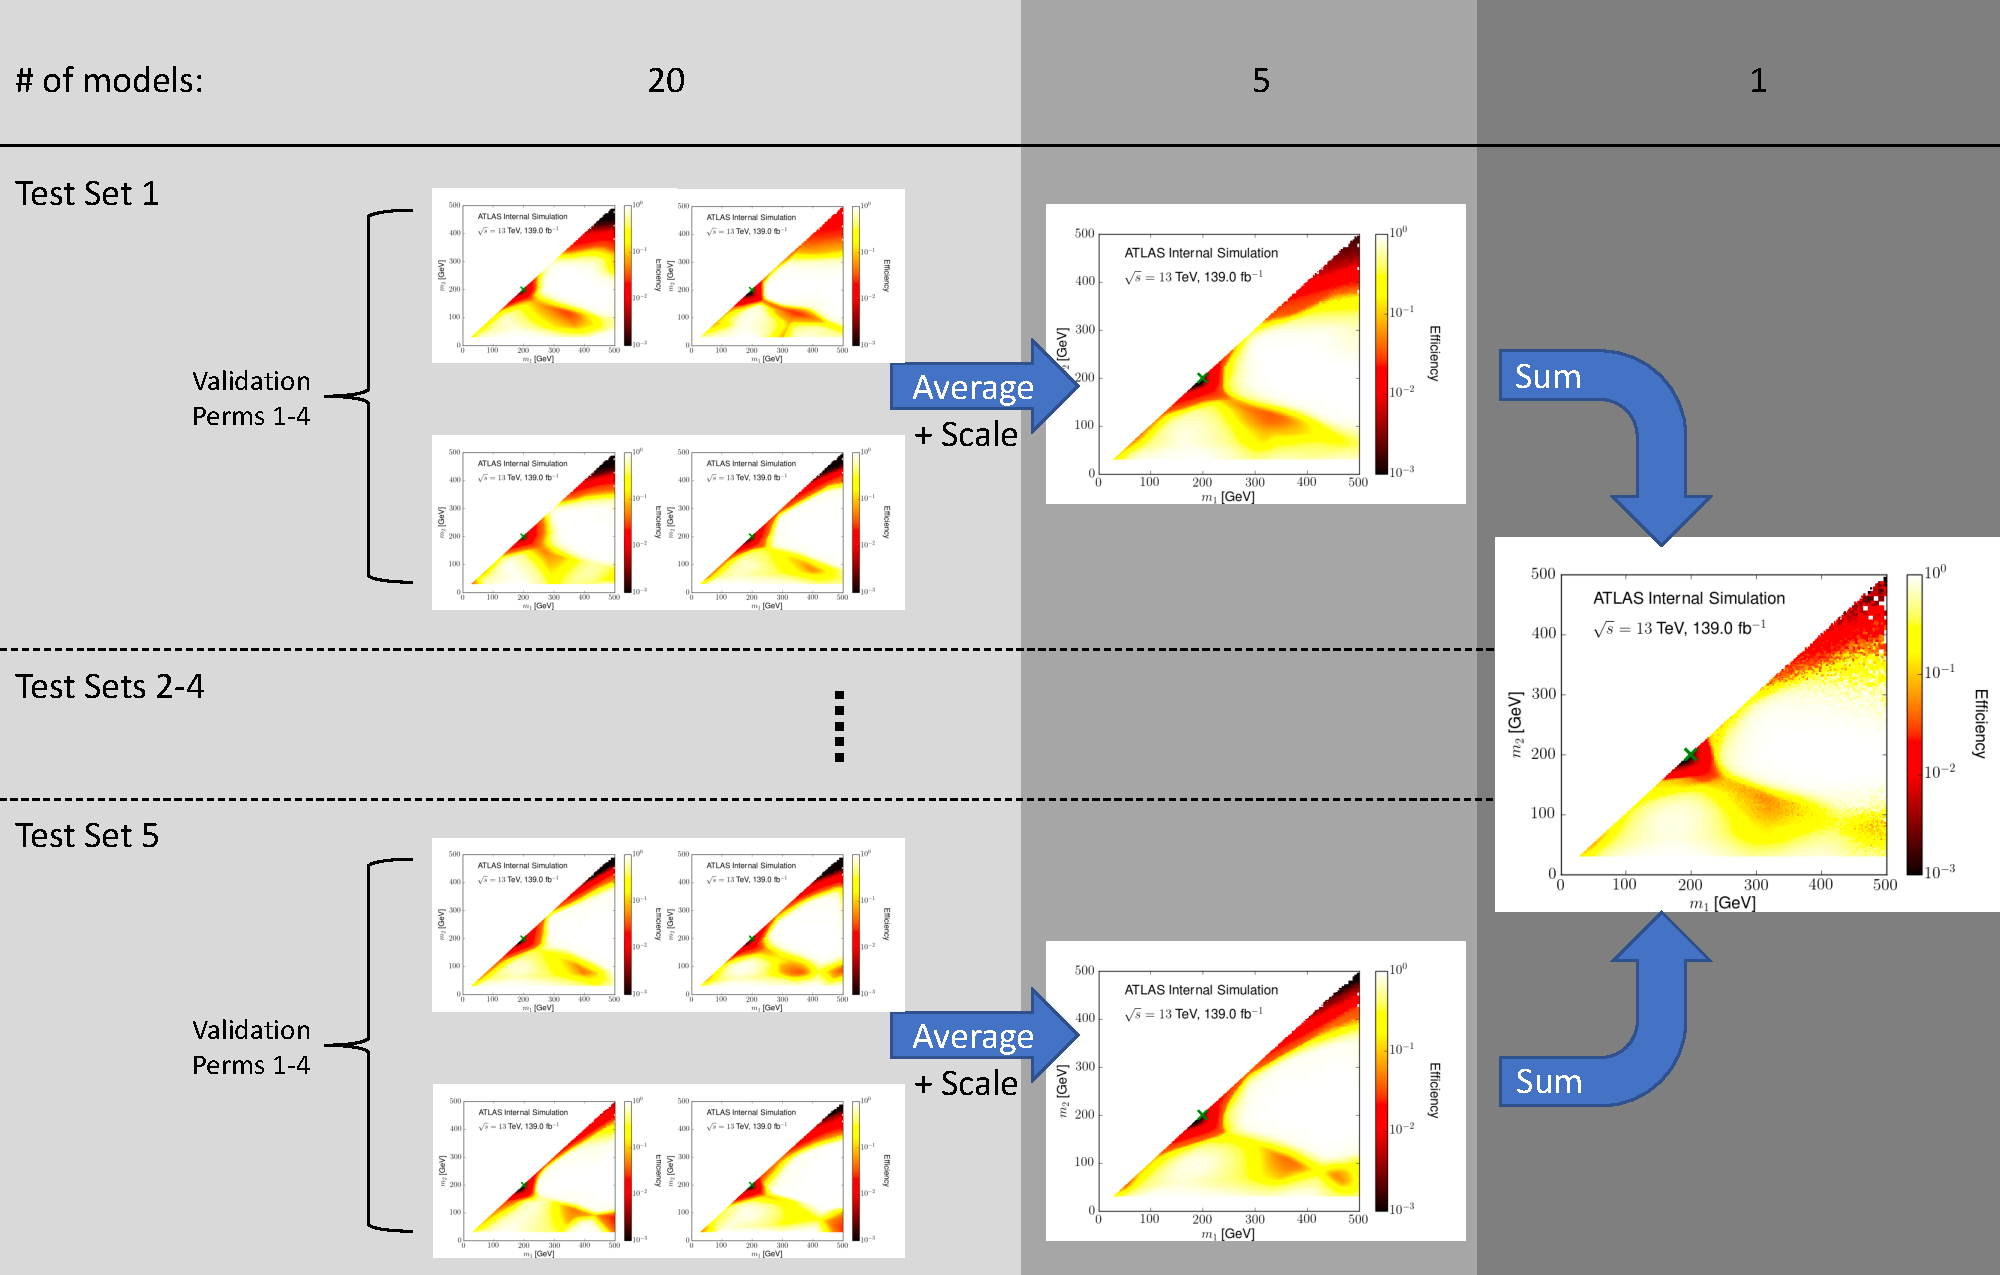
\includegraphics[width=0.9\textwidth]{figures_CWoLa/split_flowchart.pdf}
    \caption{Flowchart of steps in derivation of final network scores, as described in Section~\ref{sec:CWoLa:network}. The networks in the left-most column have already been chosen to have the lowest validation loss, as described in Step~\ref{NNstep7}. The networks are represented by a 2D plot showing the neural network output in the $m_1$,$m_2$ plane, as expressed as an efficiency on events, as described in Step~\ref{NNstep7scaling}. In this particular example, a signal was injected at $m_B=200$ GeV, $m_C=200$ GeV.  All plots in this figure use simulation.  Note that the amount of effective data in the left parts of the plot is actually $1/5$ of the total.}
    \label{fig:CWoLa:flowchart}
\end{figure}

Briefly about the trails factor in $(m_1,m_2)$: no event is selected with a classifier that was trained using that event.  The nested cross-validation is like dividing the dataset in half, training on one half and testing on the other.  The nested cross-validation extends this to use $(k-1)/k$ events for training each network (all $k$-folds get a different network) and use all events for testing. 

\subsection{Setting Limits}
\label{sec:CWoLa:limits}

The observed results are interpreted using a frequentist statistical analysis.
The parameter of interest is the signal strength, $\mu$, defined as a scale factor on the total number of signal events expected relative to some benchmark, so that $\mu=0$ corresponds to no signal, and $\mu=1$ corresponds to the benchmark.
As we do not have a specific UV model, the couplings and thus cross-sections are free parameters.  Therefore, we define the benchmark to be such that, in the benchmark model, the total number of events expected to be produced is exactly 1: $\sigma\times\text{B}\times\mathcal{L}=1$, with $\sigma$ the signal cross section for $A$ production, $\text{BR}$ the signal branching ratio to $BC$ which then decay hadronically, and $\mathcal{L}$ the data luminosity.
Then $\mu$ is exactly the total number of signal events expected to be produced.

A likelihood function $\mathcal{L}(\mu,\theta)$ is defined, with $\theta=\{\theta_s,\theta_b\}$ going over the nuisance parameters in the signal ($\theta_s$) and background ($\theta_b$).
%, and the profile likelihood ratio $\lambda(\mu)$ is used to define the discovery $p$-value $p_0$ and the exclusion $p$-value $p_\mu$~\cite{Cowan:2010js}.
The likelihood function is defined as follows:
\begin{align}
  %\mathcal{L}(\mu,\theta) = \prod_i P_\text{pois}(n_\text{obs}^i|\mu s_i + b_i)\times\mathcal{G}(\theta_s)\times\mathcal{G}(\theta_b),
  \mathcal{L}(\mu,\theta) = \prod_i P_\text{pois}(n_\text{obs}^i|\mu s_i + b_i)\times\mathcal{G}(\theta_b),
  \label{eqn:CWoLa:likelihood}
\end{align}
where $n_\text{obs}^i$ is the number of events observed in bin $i$,
$s_i$ is the fraction of signal expected in bin $i$ (including the acceptance of the trigger and the event selection),
$b_i$ is the total number of background expected in bin $i$,
as detailed in Section~\ref{sec:CWoLa:background},
%$\theta_s$ are the nuisance parameters corresponding to the systematic uncertainties on the signal shape,
and $\theta_b$ are the nuisance parameters corresponding to the uncertainty on the background fit, as described in Section~\ref{sec:CWoLa:background},
$P_\text{pois}(n|e)$ is a Poisson likelihood of $n$ events given $e$ expected, and $\mathcal{G}$ is a  Gaussian.
Note that, since $\theta_s$ only affect the shape of the signal, these uncertainties cannot be profiled.
%Furthermore, they are not included in the likelihood function directly, but are rather used as post-fit uncertainties on the derived limits, as explained below.
%\footnote{Note that the likelihood defined here is a \textit{single-bin} likelihood. We do this in order to be as agnostic as possible to the shape of the signal. Note also then that the nuisance parameters cannot be profiled.}
%and that the uncertainties on the signal normalization are degenerate with $\mu$.}

The test statistic $\lambda(\mu)$ based on the profile likelihood ratio is defined using the lowest order asymptotic approximation~\cite{Cowan:2010js}.
The significance of an observed excess with respect to the background-only hypothesis is quantified in terms of the local $p_0$, defined as the probability of the background-only model to produce an excess at least as large as the one observed.
When $p_0 = 1-\Phi(5.0) \approx 3\times10^{-7}$ (with $\Phi$ the standard normal CDF), this is called a ``discovery" of a potential new signal.
%In the absence of such an observed excess, the ``signal discovery potential strength" $\mu_{5\sigma}$ is defined to be the amount of signal such that, when injected into the data, causes an excess with a local $p_0$ small enough to claim discovery.
Exclusion limits at the 95\% confidence level, $\mu_{95}$ are also set following the CL$_s$ prescription~\cite{Read:2002hq}.

In this analysis, the cuts are not set in advance, and are rather determined by the number and nature of a potential signal.
In order to remain agnostic to the number and nature of a potential new signal, rather than optimizing the efficiency of the NN cut for a particular signal model, a few different NN cut efficiencies $\epsilon$ are chosen in order to scan the space of possible NN cuts.
These chosen efficiency values are listed in Table~\ref{tab:effs}\footnote{In the final unblinded analysis, only the values $\epsilon=0.1$ and $\epsilon=0.01$ are used.}.
\begin{table}[htb]
  \centering
  \caption{Chosen values of NN cuts with efficiency $\epsilon$ for analysis.}
  \label{tab:effs}
  \begin{tabular}{c c}
    \hline
 & Values   \\ \hline
$\epsilon$ & [1.0,0.25,0.1,0.01] \\
    \hline
  \end{tabular}
\end{table}
Each choice of $\epsilon$ is treated as a separate statistical analysis; since the choices of $\epsilon$ differ by factors of more than $2$, the results with a given NN at different values of $\epsilon$ are mostly uncorrelated.
In particular, the analysis with a cut at $\epsilon=1.0$ is very similar to the standard dijet search~\cite{ATLAS:2015nsi}, and is included as a cross-check on the results relative to existing results.

%For deriving the discovery potential $\mu_{5\sigma}$ or 95\% confidence exclusion limits $\mu_{95}$, it is necessary to inject signal on top of the background expectation in order to evaluate the profile likelihood $\lambda(\mu)$.
For deriving the 95\% confidence exclusion limits $\mu_{95}$, it is necessary to inject signal on top of the background expectation in order to evaluate the profile likelihood $\lambda(\mu)$.
The NN output depends on the presence of the signal, and in particular gets better at tagging signal the more signal there is (Appendix~\ref{sec:CWoLa:app:CWoLa:nS}). 
Therefore, the $\mu_{95}$ values are evaluated by first injecting a certain amount of signal $\mu$, running the NN training, and then performing the statistical analysis, deriving a limit $\mu_{95}(\mu)$ which is a multiple of the injected signal strength while keeping the NN fixed. 
In particular, the values $\mu_{95}(\mu)$ are functions of the injected signal strength $\mu$, derived from performing the statistical analysis after such a signal is injected.
Ideally, $\mu$ would be scanned until $\mu_{95}(\mu)=\mu\equiv\hat{\mu}_{95}$ - with this strength of signal present, that exact signal would be exluded.

However, it is expensive to scan finely over the injected $\mu$ (because of the requirement to retrain the NN at each value), so upper limits on $\hat{\mu}_{95}$ are derived by injecting a coarse grid of signal strengths $\mu$; for each analysis (validation in simulation (Section~\ref{sec:CWoLa:statanalysis}), validation in data (Section~\ref{sec:CWoLa:datastatisticalanalysis}), and unblinded (Section~\ref{sec:CWoLa:unblinded:statanalysis})) this grid is provided in the respective section.
In order to simulate a true signal, for each given injected signal strength $\mu$, exactly $\mu$ events are chosen from the given signal MC sample, with probability proportional to the MC weight.
These events are then injected into the data sample with weight $1$ and included with all the rest of the data when being passed through the steps of the analysis, in particular the event selection (Analysis Step~\ref{NNstep1}), the cross-validation splits (Section~\ref{sec:CWoLa:network}), the mass decorrelation and training (Analysis Step~\ref{NNstep5}),
However, for the tagging (Analysis Step~\ref{NNstep7}), the derived NN is applied to the entire signal sample with weights in order to get the full signal $m_{JJ}$ histogram after tagging.
The signal is injected in this way with weights $1$ for the training in order to simulate as close as possible for the NN what a true signal would look like.
The tagging is done with the full sample with the MC weights in order to derive limits as a multiple of the injected $\mu$ with the NN fixed, as described above.
For each of the $3\times4\times5=60$ (Section~\ref{sec:CWoLa:network}) iterations of the signal training, the chosen signal events injected for the NN training are held fixed.
However, for the final unblinded analysis (Section~\ref{sec:CWoLa:unblinded:statanalysis}), this entire process is repeated for $5$ different random samplings of the signal MC as a smoothing procedure, and the limit that is used for the given $\mu$ value is the limit derived from the sampling which gives the median expected limit over the $5$ random samplings.
Once a limit $\mu_{95}(\mu)$ is derived for each injected $\mu$, the final limit overall is derived as described below.

A crucial observation is that $\mu_{95}(\mu_1) \ge \mu_{95}(\mu_2)$ if $\mu_1<\mu_2$; this is because, when more signal is injected, the NN only gets better at discriminating that signal from the background, and the exclusion limit therefore only gets better (recall that the total efficiency in the signal region $\epsilon$ is fixed).
We then derive the following results:
\begin{align}
  \mu > \hat{\mu} \rightarrow \mu_{95}(\mu) \le \mu_{95}(\hat{\mu}) = \hat{\mu} < \mu \\
  \mu < \hat{\mu} \rightarrow \mu_{95}(\mu) \ge \mu_{95}(\hat{\mu}) = \hat{\mu} > \mu
\end{align}
Therefore, if $\mu>\mu_{95(\mu)}$, then $\mu$ is an appropriate upper limit on $\hat{\mu}$; and if $\mu<\mu_{95(\mu)}$, then $\mu_{95}(\mu)$ is an appropriate upper limit on $\hat{\mu}$.
In summary, with a signal injection of $\mu$, the upper limit on $\hat{\mu}$ that is set is $\text{max}\left(\mu_{95},\mu\right)$.
Since it is desirable to derive an exclusion limit as close as possible to $\hat{\mu}$, a few different values of $\mu$ are injected (depending on the signal region), and the value of $\mu$ that leads to the lowest median expected upper limit is used.

%It should be noted that, while the uncertainties on the background due to the fit parameters go directly into the likelihood (Equation~\ref{eqn:CWoLa:likelihood}) and therefore into evaluating $\mu_{95}(\mu)$, the uncertainties on the signal shape $\theta_s$ can affect the NN in an unpredictable way.
%Therefore, the effect of the systematic uncertainties that affect the signal $\theta_s$ on $\mu_{95}(\mu)$ are evaluated by running the whole procedure (including retraining the NN and varying $\mu$ to find the upper limit on $\hat{\mu}$) at discrete values of $\theta_s = \{-1,0,1\}$ and imposing a post-fit uncertainty on $\mu_{95}$.

For the global significance, one could look at the $\chi^2$ for the fit and then do a Bonferroni correction for all $m_{JJ}$ bins. It is proposed to not add this explicitly to the paper.

\subsection{Blinding Procedure}

Blinding is a challenge for two reasons.  First, blinding is a challenge for the inclusive dijet search because the event selection is inclusive by construction.  This is true for the $\epsilon=100\%$ version of this analysis.  Second, for $\epsilon < 100\%$, the event selection depends on the data, so there is no way to construct an orthogonal region ahead of time to unblind.   Our approach for these challenges is two-fold:

\begin{enumerate}
\item Run the full method in simulation.  These results are presented in Section~\ref{sec:CWoLa:simulation_analysis}.  Two challenges with this validation are (i) we have less simulation than data and (ii) the simulated events are weighted.  The latter can be challenging for our training procedure and is not an issue for the real data version of the analysis. 
\item Assuming (1) is okay, proceed to run the full method on data where the rapidity gap cut (detailed in Section~\ref{sec:CWoLa:eventselection}) is inverted.  Any $s$-channel model will have a reduced cross-section while the background rate increases.  This is discussed in Section~\ref{sec:CWoLa:val_analysis} and allows us to run the full procedure on data where we do not expect to see any signal.
\item Assuming (2) is okay, run the method on the full dataset.  The results of this are reported in Section~\ref{sec:CWoLa:unblinded}.
\end{enumerate}

\clearpage

%-------------------------------------------------------------------------------
\section{Simulation Analysis}
\label{sec:CWoLa:simulation_analysis}
%-------------------------------------------------------------------------------
In this section, the analysis is validated on a MC sample with the same event selections as will be used in data, as detailed in section~\ref{sec:CWoLa:eventselection}.

\subsection{Event Selection}
\label{sec:CWoLa:eventselection}
As mentioned in Section~\ref{sec:CWoLa:data}, data are collected using the lowest available unprescaled single-jet trigger.

For both data and simulation, the EXOT3 derivation is used, which requires at least two \\ \texttt{AntiKt10LCTopoTrimmedPtFrac5SmallR20} jets with $\pt>100$ GeV, $|\eta|<2.8$, and (uncalibrated) $m>30$ GeV if the jet $\pt$ is less than 1000 GeV.

This analysis uses anti-$k_t$, $R=1.0$ jets reconstructed from topoclusters with the local cluster weighting scheme (LCW)~\cite{Aad:2016upy}. The jets are trimmed~\cite{Krohn:2009th} using using the parameters $f_\text{cut} = 5\%$ and $R_\text{sub} = 0.2$.
A Monte Carlo-based particle-level calibration is then applied to the jets used in this analysis~\cite{Aaboud:2018kfi}.
It corrects on average the reconstructed mass and $p_T$ of the jets to their true values.
The \textit{combined mass} measurement is used, which combines measurements from the tracking system and the calorimeter; including this information has been shown to have better mass resolution, especially at high jet $\pt$~\cite{ATLAS-CONF-2016-035}.

The offline selection that is made on top of the selection from the derivation is intended to be as fully inclusive as possible to prospective signal models, while remaining on the plateau of the turn-on for the trigger.

Each event is required to have at least two \texttt{AntiKt10LCTopoTrimmedPtFrac5SmallR20} offline jets with calibrated $\pt>200$ GeV
\footnote{Jet calibrations for large-radius jets only go to 200 GeV.
In any case, the number of jets with $\pt$ between 100 and 200 GeV is negligible: 0.1\% for $m_{JJ} > 1.8$ TeV.
%The simulation and validation analyses do not remove these as they are already done and nothing noticeable will change by removing them (at the expense of a lot of additional work).  They are removed for the unblinded nominal data analysis.
}
and $|\eta|<2.0$, and with at least one such jet with calibrated $\pt>500$ GeV.
This offline threshold was shown to be fully efficient with respect to the trigger selection in the Diboson Search Support Note (ANA-HDBS-2018-31-INT1~\cite{Adorni:2647394}).
There is no explicit lepton overlap removal or veto.

Only the two jets with highest $\pt$ in the event are used in this analysis, and the remaining jets are discarded.
For each jet $j=1,2$, the four-momentum $p^\mu_j$ recorded, in particular the jet mass $m_j^2 = (p^\mu_j)^2$.
In order to suppress contributions from $t$-channel QCD dijet production, while remaining efficient on $A\rightarrow BC$ signals, a selection is placed on the rapidity difference, $|y_1-y_2|<1.2$.
The distribution of the rapidity difference in the background can be seen in Figure~\ref{fig:CWoLa:bkg_rapdiff}, and the distributions in various signal models can be seen in Figure~\ref{fig:CWoLa:sig_rapdiff}.

\begin{figure}[htbp]
  \centering 
  \subfloat[]{\includegraphics[width=0.45\textwidth]{figures_CWoLa/{jet_rapdiff_log_bn04_4.10.19}.pdf}}
  \subfloat[]{\includegraphics[width=0.45\textwidth]{figures_CWoLa/{jet_rapdiff_log_bn510_4.10.19}.pdf}}
  \caption{Distribution of $|y_1-y_2|$ in the background, broken down by the $m_{JJ}$ region, as described in Section~\ref{sec:CWoLa:binning}. (a) $m_{JJ}$ regions 0-4; (b) $m_{JJ}$ regions 5-9. The green line indicates the cut at 1.2.}
\label{fig:CWoLa:bkg_rapdiff}
\end{figure}

\begin{figure}[htbp]
  \centering 
  \subfloat[]{\includegraphics[width=0.45\textwidth]{figures_CWoLa/{jet_rapdiff_log_Wprime_WZqqqq_M3000_m200_m200_4.10.19}.pdf}}
  %\subfloat[]{\includegraphics[width=0.45\textwidth]{figures_CWoLa/{jet_rapdiff_log_Wprime_WZqqqq_M6000_m200_m200_4.10.19}.pdf}}
  \caption{Distribution of $|y_1-y_2|$ for a signal model with ($m_A,m_B,m_C=3000,200,200$ GeV).
    %(a) ($m_A,m_B,m_C=3000,200,200$ GeV);
    %(b) ($m_A,m_B,m_C=6000,200,200$ GeV).
    The green line indicates the cut at 1.2.}
\label{fig:CWoLa:sig_rapdiff}
\end{figure}

The jets are ordered by their mass, so that $m_1 \ge m_2$.
In order to suppress background and therefore increase sensitivity to massive signal objects, a minimum cut $m_1$, $m_2 > 30 \GeV$ is applied.
Also, in order to make the kinematic region in which the learning is applied definite, as discussed in Section~\ref{sec:CWoLa:features}, a maximum cut $m_1$, $m_2 < 500 \GeV$ is applied.

Typically the dijet invariant mass $m_{JJ}$ would be defined as in terms of the sum of the four-momenta of the two jets, $m_{JJ}^2 = (p^\mu_1+p^\mu_2)^2 = m_1^2+m_2^2+2\left(E_1E_2-\vec{p}_1\cdot\vec{p}_2\right)$, with $E^2 = |\vec{p}|^2+m^2$ and $|\vec{p}| = p_T\cosh(\eta)$.
In this analysis the dijet invariant mass is defined slightly differently: in order to reduce correlations between the features used in the neural network ($m_1,m_2$) and the final $m_{JJ}$ value, the dijet invariant mass is formed by setting all $m_i$ to zero: $m_{JJ}^2 \equiv 2\left(|\vec{p}_1||\vec{p_2}|-\vec{p}_1\cdot\vec{p}_2\right)$.
This new definition removes all correlations between $m_{JJ}$ and $m_1,m_2$ except for those arising from indirect correlations between the jet $m$ and the jet $p_T$ and $\eta$.
In practice this is a very small change, because the jets in this analysis typically have energies much larger than their masses, and so the new definition gives almost the same value for the invariant mass.
As discussed in Section~\ref{sec:CWoLa:binning}, a selection is applied on the dijet invariant mass of $1.1 \le m_{JJ} < 8.17$ TeV.
In the analyses in data, both the validation selection (Section~\ref{sec:CWoLa:val_analysis}) and the final signal selection (Section~\ref{sec:CWoLa:unblinded}), effectively a selection of $1.8 \le m_{JJ} < 8.2$ TeV is applied as the fitting range.

These selections are summarized in Table~\ref{tab:event_selection}.
\begin{table}[htbp]
  \begin{center}
    \caption{Jet selection. The $m_{JJ}$ selection is indicated for the simulation-based analysis (Section~\ref{sec:CWoLa:simulation_analysis}), and in parentheses for the validation selection analysis (Section~\ref{sec:CWoLa:val_analysis}) and for the signal selection analysis (Section~\ref{sec:CWoLa:unblinded}).}
  \label{tab:event_selection}
    \begin{tabular}{c c}
      \hline
      Observable & Selection \\
      \hline
      $p_T$ & $>500$ GeV (leading), $>200$ GeV (subleading) \\
      $|\eta|$ & $<2.0$ \\
      $|y_1-y_2|$ & $<1.2$ \\
      $m$ & $> 30$ GeV, $<500$ GeV \\
      $m_{JJ}$ & $\ge 1.1 (1.8)$ TeV, $<8.17 (8.2)$ TeV \\
      \hline
    \end{tabular}
  \end{center}
\end{table}

The cutflow of these selections on the signal samples is given in Table~\ref{tab:cutflow_signal}.
\begin{table}[htbp]
  \begin{center}
    \caption{Signal sample efficiency with selections up to and including given selection. All selections are given in Section~\ref{sec:CWoLa:eventselection}. The jet selections are summarized in Table~\ref{tab:event_selection}. The $m_{JJ}$ selection is included for a selection of $1.1 \le m_{JJ} < 8.17$ TeV and for a selection of $1.8 \le m_{JJ} < 8.2$ TeV, indicated by the lower end of the selection.}
  \label{tab:cutflow_signal}
    \begin{tabular}{c c c c c c c c c}
      \hline
      $(m_A,m_B,m_C)$ [\GeV] & Derivation & Trigger & \pt & $|\eta|$ & $|y_1-y_2|$ & $m$ & $m_{JJ}$ ($1.1$ \TeV) & $m_{JJ}$ ($1.8$ \TeV) \\
      \hline
      (3000,80,80)   & 1.00 & 0.90 & 0.85 & 0.85 & 0.64 & 0.63 & 0.62 & 0.59 \\
      (3000,80,200)  & 1.00 & 0.91 & 0.85 & 0.85 & 0.63 & 0.62 & 0.61 & 0.58 \\
      (3000,80,400)  & 1.00 & 0.92 & 0.81 & 0.81 & 0.61 & 0.60 & 0.58 & 0.56 \\
      (3000,200,200) & 1.00 & 0.93 & 0.87 & 0.87 & 0.64 & 0.63 & 0.63 & 0.59 \\
      (3000,200,400) & 1.00 & 0.95 & 0.84 & 0.84 & 0.62 & 0.61 & 0.60 & 0.58 \\
      (3000,400,400) & 1.00 & 0.95 & 0.82 & 0.82 & 0.62 & 0.60 & 0.59 & 0.57 \\
      (5000,80,80)   & 1.00 & 0.68 & 0.58 & 0.58 & 0.44 & 0.44 & 0.42 & 0.34 \\
      (5000,80,200)  & 1.00 & 0.70 & 0.59 & 0.59 & 0.45 & 0.44 & 0.42 & 0.34 \\
      (5000,80,400)  & 1.00 & 0.78 & 0.58 & 0.58 & 0.44 & 0.43 & 0.40 & 0.34 \\
      (5000,200,200) & 1.00 & 0.75 & 0.63 & 0.63 & 0.48 & 0.47 & 0.45 & 0.37 \\
      (5000,200,400) & 1.00 & 0.82 & 0.65 & 0.65 & 0.49 & 0.48 & 0.45 & 0.39 \\
      (5000,400,400) & 1.00 & 0.88 & 0.68 & 0.68 & 0.50 & 0.48 & 0.47 & 0.43 \\
      \hline
    \end{tabular}
  \end{center}
\end{table}

\subsection{Binning}
\label{sec:CWoLa:binning}
The $m_{JJ}$ spectrum is binned in order to derive the signal and sideband regions.
The size of the binning is chosen to be 20\%, guided by the dijet mass resolution that would arise from a narrow signal peak.
The minimum $m_{JJ}$ value is 1.1 TeV, due to the jet and trigger selection, and the maximum value is at 8.17 TeV (the right edge of bin $10$ with 20\% bin size), above which few events are expected to be observed.
Since every event is required to lie in an $m_{JJ}$ bin, effectively an event selection is therefore applied for $1.1 \le m_{JJ} < 8.17$ TeV.
The bin definitions are given in Table~\ref{tab:mjj_bins}.

\begin{table}[htb]
  \centering
  \caption{\label{tab:mjj_bins} $m_{JJ}$ bin definitions.}
  \begin{tabular}{c c}
    \hline
    Bin & Definition  \\ \hline
    0 & $1.10 \le m_{JJ} < 1.32$ TeV \\
    1 & $1.32 \le m_{JJ} < 1.58$ TeV \\
    2 & $1.58 \le m_{JJ} < 1.90$ TeV \\
    3 & $1.90 \le m_{JJ} < 2.28$ TeV \\
    4 & $2.28 \le m_{JJ} < 2.74$ TeV \\
    5 & $2.74 \le m_{JJ} < 3.28$ TeV \\
    6 & $3.28 \le m_{JJ} < 3.94$ TeV \\
    7 & $3.94 \le m_{JJ} < 4.73$ TeV \\
    8 & $4.73 \le m_{JJ} < 5.68$ TeV \\
    9 & $5.68 \le m_{JJ} < 6.81$ TeV \\
    10 & $6.81 \le m_{JJ} < 8.17$ TeV \\
    \hline
  \end{tabular}
\end{table}

The distribution of $m_{JJ}$ in the background with these bin definitions can be seen in Figure~\ref{fig:CWoLa:bkg_mjj}.
It can be seen that the distribution of $m_{JJ}$ in the background before any cuts is smooth, with no bumps indicating possible discoveries.
\begin{figure}[htbp]
  \centering 
  \subfloat[]{\includegraphics[width=0.6\textwidth]{figures_CWoLa/{mjj_loglog_4.10.19}.pdf}}
  \caption{Distribution of $m_{JJ}$ in the background MC. The green lines indicate the bin edges of $m_{JJ}$ regions 0-10.}
\label{fig:CWoLa:bkg_mjj}
\end{figure}

The distributions of $m_{JJ}$ in a variety of signal models are plotted in Figure~\ref{fig:CWoLa:sig_mjj}.
It can be seen that the mass of the signal object, $m_A$, is well-reconstructed as $m_{JJ}$, with significant tails at lower $m_{JJ}$ values.
The resolution of $m_A$ with $m_{JJ}$ is roughly 20\%, which guides the sizing of the binning, as mentioned above.

\begin{figure}[htbp]
  \centering 
  \subfloat[]{\includegraphics[width=0.3\textwidth]{figures_CWoLa/{mjj_loglog_vlines_Wprime_WZqqqq_M3000_m80_m80_1.14.20}.pdf}}
  \subfloat[]{\includegraphics[width=0.3\textwidth]{figures_CWoLa/{mjj_loglog_vlines_Wprime_WZqqqq_M3000_m80_m200_1.14.20}.pdf}}
  \subfloat[]{\includegraphics[width=0.3\textwidth]{figures_CWoLa/{mjj_loglog_vlines_Wprime_WZqqqq_M3000_m80_m400_1.14.20}.pdf}}\\
  \subfloat[]{\includegraphics[width=0.3\textwidth]{figures_CWoLa/{mjj_loglog_vlines_Wprime_WZqqqq_M3000_m200_m200_1.14.20}.pdf}}
  \subfloat[]{\includegraphics[width=0.3\textwidth]{figures_CWoLa/{mjj_loglog_vlines_Wprime_WZqqqq_M3000_m200_m400_1.14.20}.pdf}}
  \subfloat[]{\includegraphics[width=0.3\textwidth]{figures_CWoLa/{mjj_loglog_vlines_Wprime_WZqqqq_M3000_m400_m400_1.14.20}.pdf}}\\
  \subfloat[]{\includegraphics[width=0.3\textwidth]{figures_CWoLa/{mjj_loglog_vlines_Wprime_WZqqqq_M5000_m80_m80_1.14.20}.pdf}}
  \subfloat[]{\includegraphics[width=0.3\textwidth]{figures_CWoLa/{mjj_loglog_vlines_Wprime_WZqqqq_M5000_m80_m200_1.14.20}.pdf}}
  \subfloat[]{\includegraphics[width=0.3\textwidth]{figures_CWoLa/{mjj_loglog_vlines_Wprime_WZqqqq_M5000_m80_m400_1.14.20}.pdf}}\\
  \subfloat[]{\includegraphics[width=0.3\textwidth]{figures_CWoLa/{mjj_loglog_vlines_Wprime_WZqqqq_M5000_m200_m200_1.14.20}.pdf}}
  \subfloat[]{\includegraphics[width=0.3\textwidth]{figures_CWoLa/{mjj_loglog_vlines_Wprime_WZqqqq_M5000_m200_m400_1.14.20}.pdf}}
  \subfloat[]{\includegraphics[width=0.3\textwidth]{figures_CWoLa/{mjj_loglog_vlines_Wprime_WZqqqq_M5000_m400_m400_1.14.20}.pdf}}\\
  \caption{Distribution of $m_{JJ}$ for a signal model with
    (a) ($m_A,m_B,m_C=3000,80,80$ GeV);
    (b) ($m_A,m_B,m_C=3000,200,80$ GeV);
    (c) ($m_A,m_B,m_C=3000,400,80$ GeV);
    (d) ($m_A,m_B,m_C=3000,200,200$ GeV);
    (e) ($m_A,m_B,m_C=3000,400,20$ GeV);
    (f) ($m_A,m_B,m_C=3000,400,400$ GeV).
    (g) ($m_A,m_B,m_C=5000,80,80$ GeV);
    (h) ($m_A,m_B,m_C=5000,200,80$ GeV);
    (i) ($m_A,m_B,m_C=5000,400,80$ GeV);
    (j) ($m_A,m_B,m_C=5000,200,200$ GeV);
    (k) ($m_A,m_B,m_C=5000,400,20$ GeV);
    (l) ($m_A,m_B,m_C=5000,400,400$ GeV).
  }
\label{fig:CWoLa:sig_mjj}
\end{figure}

One thing to note about this analysis is that the binnings are fixed.
A possible issue with this is that for a signal that is found close to the edge of a bin, the NN may not learn to tag that signal because it has presence in both that bin and its sideband.
This effect is mitigated somewhat due to two factors: (1) Because the background is steeply falling, there is only a small region of $m_A$ in which the signal fraction in both a signal bin and its sideband are comparable; and (2) the NN is trained on both sidebands simultaneously, so that the signal should still be tagged when distinguishing between the signal region and the combined sidebands even if it lies on the edge.
A study of this effect is presented in Appendix~\ref{app:CWoLa:binoffset}.

\subsection{Sensitivity to Signals}

Some thorough studies are performed to test the sensitivity of the neural network to various signals.
%In Appendix~\ref{sec:CWoLa:app:CWoLa:NNout_bkg}, the neural network scores are shown for a background-only sample with no injected signal.
In Section~\ref{sec:CWoLa:app:CWoLa:vary_signal}, the neural network scores are shown for a sample with injected signal at a variety of points in the $m_A,m_B,m_C$ space.
In Section~\ref{sec:CWoLa:app:CWoLa:nS}, the neural network scores are shown for a particular signal sample, with the signal strength varying to show how the network learns about the presence of signal for a large enough signal.

\subsubsection{Sensitivity of Neural Network to Different Signal Samples}
\label{sec:CWoLa:app:CWoLa:vary_signal}
A study is performed by training the neural network with different injected signals in different part of the $m_A,m_B,m_C$ kinematic space, for fixed $\mu$.

For $m_A=3000$ GeV, this signal lies in signal region 5.
In this region, there are roughly $1.0\times10^5$ background events, and $\mu$ is set to 1500; after all event selections ($~45\%$ efficiency), there are roughly $650$ signal events in signal region 5, for a signal fraction of $\sim 0.7\%$ and an estimated significance $\frac{S}{\sqrt{B}}$ $\sim 2$.
The results of this study can be seen in Figure~\ref{fig:CWoLa:vary_signal_sigR5}.
The network succesfully learns to tag the kinematic region near the true signal as being signal-like.

\begin{figure}[htbp]
  \centering 
  \subfloat[]{\includegraphics[width=0.3\textwidth]{figures_CWoLa/{NNoutcontrast_sigR5_Wprime_WZqqqq_M3000_m80_m80_nS1500_patience1000_4.10.19}.png}}
  \subfloat[]{\includegraphics[width=0.3\textwidth]{figures_CWoLa/{NNoutcontrast_sigR5_Wprime_WZqqqq_M3000_m80_m200_nS1500_patience1000_4.10.19}.png}}
  \subfloat[]{\includegraphics[width=0.3\textwidth]{figures_CWoLa/{NNoutcontrast_sigR5_Wprime_WZqqqq_M3000_m80_m400_nS1500_patience1000_4.10.19}.png}}\\
  \subfloat[]{\includegraphics[width=0.3\textwidth]{figures_CWoLa/{NNoutcontrast_sigR5_Wprime_WZqqqq_M3000_m200_m200_nS1500_patience1000_4.10.19}.png}}
  \subfloat[]{\includegraphics[width=0.3\textwidth]{figures_CWoLa/{NNoutcontrast_sigR5_Wprime_WZqqqq_M3000_m200_m400_nS1500_patience1000_4.10.19}.png}}
  \subfloat[]{\includegraphics[width=0.3\textwidth]{figures_CWoLa/{NNoutcontrast_sigR5_Wprime_WZqqqq_M3000_m400_m400_nS1500_patience1000_4.10.19}.png}}
  \caption{Neural network output for signal region 5 with $\mu=1500$ for a signal with $m_A=3000$ GeV and
  (a) ($m_B,m_C = 80,80$ GeV);
  (b) ($m_B,m_C = 200,80$ GeV);
  (c) ($m_B,m_C = 400,80$ GeV);
  (d) ($m_B,m_C = 200,200$ GeV);
  (e) ($m_B,m_C = 400,200$ GeV);
  (f) ($m_B,m_C = 400,400$ GeV).
  }
\label{fig:CWoLa:vary_signal_sigR5}
\end{figure}

%For $m_A=6000$ GeV, this signal lies mostly in signal region 9, but there is significant bleeding into signal region 8.
%In signal region 9, there are roughly $3900$ background events, and $\mu$ is set to 5000; after all event selections ($~50\%$ efficiency), there are roughly 450 signal events in signal region 9, for a signal fraction of roughly $12\%$.
%The results of this study in signal region 9 can be seen in Figure~\ref{fig:CWoLa:vary_signal_sigR9}.
%The network succesfully learns to tag the kinematic region near the true signal as being signal-like.
%In signal region 8, there are roughly $25000$ background events; after all event selections, there are roughly 250 signal events in signal region 8, for a a signal fraction of roughly $1\%$.
%The results of this study in signal region 8 can be seen in Figure~\ref{fig:CWoLa:vary_signal_sigR8}.
%The network succesfully learns to anti-tag the kinematic region near the true signal as being signal-like, since training on signal region 8 falls under Case~\ref{case2}.
%
%\begin{figure}[htbp]
%  \centering 
%  \subfloat[]{\includegraphics[width=0.3\textwidth]{figures_CWoLa/{NNout_sigR9_Wprime_WZqqqq_M6000_m80_m80_nS5000_12.31.18}.png}}
%  \subfloat[]{\includegraphics[width=0.3\textwidth]{figures_CWoLa/{NNout_sigR9_Wprime_WZqqqq_M6000_m80_m200_nS5000_12.31.18}.png}}
%  \subfloat[]{\includegraphics[width=0.3\textwidth]{figures_CWoLa/{NNout_sigR9_Wprime_WZqqqq_M6000_m80_m400_nS5000_12.31.18}.png}}\\
%  \subfloat[]{\includegraphics[width=0.3\textwidth]{figures_CWoLa/{NNout_sigR9_Wprime_WZqqqq_M6000_m200_m200_nS5000_12.31.18}.png}}
%  \subfloat[]{\includegraphics[width=0.3\textwidth]{figures_CWoLa/{NNout_sigR9_Wprime_WZqqqq_M6000_m200_m400_nS5000_12.31.18}.png}}
%  \subfloat[]{\includegraphics[width=0.3\textwidth]{figures_CWoLa/{NNout_sigR9_Wprime_WZqqqq_M6000_m400_m400_nS5000_12.31.18}.png}}\\
%  \caption{Neural network output for signal region 9 with $\mu=5000$ for a signal with $m_A=6000$ GeV and
%  (a) ($m_B,m_C = 80,80$ GeV);
%  (b) ($m_B,m_C = 200,80$ GeV);
%  (c) ($m_B,m_C = 400,80$ GeV);
%  (d) ($m_B,m_C = 200,200$ GeV);
%  (e) ($m_B,m_C = 400,200$ GeV);
%  (f) ($m_B,m_C = 400,400$ GeV).
%Blue indicates more signal-like.}
%\label{fig:CWoLa:vary_signal_sigR9}
%\end{figure}
%
%\begin{figure}[htbp]
%  \centering 
%  \subfloat[]{\includegraphics[width=0.3\textwidth]{figures_CWoLa/{NNout_sigR8_Wprime_WZqqqq_M6000_m80_m80_nS5000_12.31.18}.png}}
%  \subfloat[]{\includegraphics[width=0.3\textwidth]{figures_CWoLa/{NNout_sigR8_Wprime_WZqqqq_M6000_m80_m200_nS5000_12.31.18}.png}}
%  \subfloat[]{\includegraphics[width=0.3\textwidth]{figures_CWoLa/{NNout_sigR8_Wprime_WZqqqq_M6000_m80_m400_nS5000_12.31.18}.png}}\\
%  \subfloat[]{\includegraphics[width=0.3\textwidth]{figures_CWoLa/{NNout_sigR8_Wprime_WZqqqq_M6000_m200_m200_nS5000_12.31.18}.png}}
%  \subfloat[]{\includegraphics[width=0.3\textwidth]{figures_CWoLa/{NNout_sigR8_Wprime_WZqqqq_M6000_m200_m400_nS5000_12.31.18}.png}}
%  \subfloat[]{\includegraphics[width=0.3\textwidth]{figures_CWoLa/{NNout_sigR8_Wprime_WZqqqq_M6000_m400_m400_nS5000_12.31.18}.png}}\\
%  \caption{Neural network output for signal region 8 with $\mu=5000$ for a signal with $m_A=6000$ GeV and
%  (a) ($m_B,m_C = 80,80$ GeV);
%  (b) ($m_B,m_C = 200,80$ GeV);
%  (c) ($m_B,m_C = 400,80$ GeV);
%  (d) ($m_B,m_C = 200,200$ GeV);
%  (e) ($m_B,m_C = 400,200$ GeV);
%  (f) ($m_B,m_C = 400,400$ GeV).
%Blue indicates more signal-like.}
%\label{fig:CWoLa:vary_signal_sigR8}
%\end{figure}


\subsubsection{Sensitivity of Neural Network to $\mu$}
\label{sec:CWoLa:app:CWoLa:nS}
A study is performed with a fixed signal model ($m_{JJ} = 3000$ GeV; $m_B,m_C = 200,400$ GeV), varying $\mu$ in order to test the sensitivity of the neural network to $\mu$.
This signal lies in signal region 5; the results when training with signal region 5 as the signal region can be seen in Figure~\ref{fig:CWoLa:nS_study}.
There are roughly $1.0\times10^5$ background events in this signal region; the signal fraction and estimated significance varies from $\sim 0.3\%$, $\sim 1$ (at $\mu=750$), respectively, to $0.7\%$, $\sim 2$ (at $\mu=1500$), respectively.
For low $\mu$, the network is unable to detect the presence of the signal, and it learns to tag the same kinematic regions as in the background-only case.
As $\mu$ increases, the network becomes more confident about tagging the kinematic region near the true signal, while still tagging the kinematic regions that are present in the background-only case.
%In particular, there seems to be a sharp turn-on, somewhere between $\mu=10000$ and $\mu=20000$, where the network learns to tag the kinematic region near the true signal.

\begin{figure}[htbp]
  \centering 
  \subfloat[]{\includegraphics[width=0.45\textwidth]{figures_CWoLa/{NNoutcontrast_sigR5_patience1000_4.10.19}.png}}
  \subfloat[]{\includegraphics[width=0.45\textwidth]{figures_CWoLa/{NNoutcontrast_sigR5_Wprime_WZqqqq_M3000_m200_m400_nS750_patience1000_4.10.19}.png}}\\
  \subfloat[]{\includegraphics[width=0.45\textwidth]{figures_CWoLa/{NNoutcontrast_sigR5_Wprime_WZqqqq_M3000_m200_m400_nS1000_patience1000_4.10.19}.png}}
  \subfloat[]{\includegraphics[width=0.45\textwidth]{figures_CWoLa/{NNoutcontrast_sigR5_Wprime_WZqqqq_M3000_m200_m400_nS1500_patience1000_4.10.19}.png}}\\
  \caption{Neural network output for signal region 5 with a signal at ($m_A,m_B,m_C = 3000,200,400$ GeV) with (a) $\mu=0$; (b) $\mu=750$; (c) $\mu=1000$; (d) $\mu=1500$.}
\label{fig:CWoLa:nS_study}
\end{figure}

\subsection{Background Fitting}
\label{sec:CWoLa:background}

After the application of the CWoLa training described above, a standard parametric background fit is performed to estimate the background contribution in the signal region.  The selected fit function is the same as the one used by the all-hadronic diboson resonance search:

\begin{align}
\label{eqn:CWoLa:fitfunction}
\frac{dn}{dx}=p_1(1-x)^{p_2-\xi p_3}x^{-p_3},
\end{align}

\noindent where $x=m_{JJ}/\sqrt{s}$, $p_1$ is a normalization parameter, $p_2$ and $p_3$ are dimensionless shape parameters, and $\xi$ is a constant (not varied in the fit).  For simplicity, we set $\xi=0$ (in the diboson search, it is chosen to reduce correlations between $p_2$ and $p_3$).  Example fits in the coarse bins used for training are shown in Figure~\ref{fig:CWoLa:examplefits}.  More details of the fitting and its interplay with the statistical interpretation can be found in the next section.  The fitting procedure was tweaked for the data analysis, as described in Section~\ref{sec:CWoLa:inverted:datafitting}.

\begin{figure}[h!]
    \centering
    \subfloat[]{\includegraphics[width=0.45\textwidth]{figures_CWoLa/{mjj_loglog_fit_all_sigR5_Wprime_WZqqqq_M3000_m200_m200_nS1500_patience1000_SEC_4params_4.10.19}.pdf}}
    \subfloat[]{\includegraphics[width=0.45\textwidth]{figures_CWoLa/{mjj_loglog_fit_q99_sigR5_Wprime_WZqqqq_M3000_m200_m200_nS1500_patience1000_SEC_4params_4.10.19}.pdf}}
    \caption{Example fits to the $m_{JJ}$ spectrum using the functional form given in Equation~\ref{eqn:CWoLa:fitfunction}.
    There is an injected signal sample at $m_A,m_B,m_C=3000,200,200$ GeV, which lies mostly in signal segion 5, and with $\frac{S}{\sqrt{B}}\sim 2$ in that region. (a) With no cut on the NN output; (b) Training a NN with signal region $s=5$ ($2.74-3.28$~\TeV), and making a cut on the NN output at efficiency $\epsilon=0.01$.   The uncertainty on the fit is due to the covariance matrix from the fit parameters.}
    \label{fig:CWoLa:examplefits}
\end{figure}

\subsection{Statistical Analysis}
\label{sec:CWoLa:statanalysis}

The statistical analysis uses the \href{https://gitlab.cern.ch/atlas-phys/exot/dbl/ResonanceFinder}{\texttt{ResonanceFinder}} package from the DBL group.  This code is based on RooFit~\cite{Verkerke:2003ir}, RooStats~\cite{Moneta:2010pm}, and HistFactory~\cite{Cranmer:1456844}.  For the simulation analysis, there were not modifications to the methodology used by the all-hadronic diboson resonance analysis.  Modifications for the data analysis can be found in Section~\ref{sec:CWoLa:datastatisticalanalysis} for the actual statistical setup and Section~\ref{sec:CWoLa:inverted:datafitting} for the background fitting.

The core ideas for the statistical analysis can be found in Section~\ref{sec:CWoLa:limits} and the specific implementation details are described here.  First, given the simulation after a cut on the NN (or not), a parametric fit is performed using 100 GeV bins from 2 TeV to 8.2 TeV, with 69 bins total\footnote{The 8.2 TeV maximum bin edge contains the 8.17 TeV maximum $m_{JJ}$ from the event selection (Section~\ref{sec:CWoLa:eventselection}); this value is essentially arbitrary as there are expected to be $<1$ events at that high $m_{JJ}$.}.  These bins are finer than the bins used for learning and described in Section~\ref{sec:CWoLa:binning}.  The fit function is the one from Section~\ref{sec:CWoLa:background}, with $\xi=4.2955$, as used by the all-hadronic diboson resonance search.  The parameter $p_2$ is initialized to 10 and restricted to the range $[-100,100]$ and the parameter $p_3$ is initialized to $-30$ and restricted to the range $[-100,100]$ as well.  The signal region is not masked during this fit.  After the fit, the prediction is normalized to have the same integral as the data over the entire range.  As there are two free parameters, the fit produces a $2\times 2$ covariance matrix.  

As described in Section~\ref{sec:CWoLa:limits}, there is a coarse scan of injected $\mu$ values to train the NN, following which, for each injected $\mu$, limits are set following the CL$_s$ procedure by scanning the overall signal strength as the POI while keeping the NN fixed.
The values of $\mu$ injected for this analysis are given in Table~\ref{tab:MC:injectedmu}.

\begin{table}[htb]
  \centering
  \caption{Injected $\mu$ values.}
  \label{tab:MC:injectedmu}
  \begin{tabular}{c c c}
    \hline
    Bin & $m_a$ [GeV] & Values \\ \hline
    5 & 3000 & [750,1000,1500,2000] \\
    \hline
  \end{tabular}
\end{table} 

The background fit is decoupled from the POI scan.  A background prediction is generated as a histogram from the central values of the background fit.  There is one nuisance parameter for the background fit systematic uncertainty.  The `up' and `down' variations are created by taking the sum in quadrature of the uncertainties from the two parameters from the original background fit ($p_2$ and $p_3$).  This nuisance parameter can be profiled in the second fit used to fit the POI.   

\subsection{Results}

%We also note that the all-hadronic diboson resonance search analysis team\footnote{We are grateful to Roland Jansky and Kalliopi Iordanidou for performing this test.} has also tested our benchmark signals and as expected, have an excellent sensitivity to the benchmark near $(m_{Z/W},m_{Z/W})$ but no sensitivity away from this point due to the mass requirements used in the analysis.

The 95\% confidence exclusion limit $\mu_{95}$ on a variety of signal models is shown in Figure~\ref{fig:CWoLa:sigma95}, expressed as the limit on the cross section times branching ratio, $\sigma_{95}\times B = \frac{\mu_{95}}{\mathcal{L}}$, where $\mathcal{L} = 139$~fb$^{-1}$ is the total integrated luminosity.
The result is shown for a few different values of $\epsilon$, where the NN is trained with signal region $s=5$, which is the signal region in which these signal models mostly lie.
For comparison, we also show limits for the all-hadronic diboson resonance search\footnote{We are grateful to Roland Jansky and Kalliopi Iordanidou for performing this test.} and for the inclusive dijet search\footnote{We are grateful to Binbin Dong for performing this test.}.
For these additional limits, the signal samples for this analysis were passed through the analysis frameworks of the diboson and inclusive dijet searches.
In particular, small-radius jets were used for the inclusive dijet search.

The $\epsilon=1$ regime of the search has no machine learning tagging and is therefore similar to the inclusive dijet search.
The limits from the $\epsilon=1$ search are about the same as the inclusive dijet search for lower $m_B,m_C$; but they are much better at higher $m_B,m_C$, because small-radius jets are often not sufficient to contain all of the decay products of the daughter resonances.
The comparison between the diboson resonance search and the inclusive dijet search is performed for the first time in the rightmost column of Figure~\ref{fig:CWoLa:sigma95}.
As expected. the targeted diboson search is more sensitive and the difference in limits is about a factor of 10.
Away from the SM dibosons, CWoLa hunting with $\epsilon<1$ outperforms the other searches by as much as a factor of five for the heaviest masses.

%sample:                               observed limit[pb], expected limit[pb]:
%3TeV_80GeV_80GeV:       0.00713022,            0.00584819
%3TeV_80GeV_200GeV:     0.00785234,           0.00674434
%3TeV_80GeV_400GeV:     0.0182049,             0.015643
%3TeV_200GeV_200GeV:   0.00805465,           0.00699676
%3TeV_200GeV_400GeV:   0.0183346,             0.0161542
%3TeV_400GeV_400GeV:   0.0260437,             0.0282762

%6TeV_80GeV_80GeV:       0.000726661,         0.00105962
%6TeV_80GeV_200GeV:     0.000796257,         0.001029
%6TeV_80GeV_400GeV:     0.0012986,             0.00162539
%6TeV_200GeV_200GeV:   0.000661496,         0.00089748
%6TeV_200GeV_400GeV:   0.000877514,         0.00109904
%6TeV_400GeV_400GeV:   0.000862185,         0.00108135

%From Roland
%So, for m = 80 GeV CWoLa signals:
%CwoLa expected limits:
%3TeV	0.6182026
%6TeV  1.0625823

%Radion expected limits:
%3TeV  0.7855590
%6TeV  0.2351363

\begin{figure}[h!]
    \centering
    \includegraphics[width=0.9\textwidth]{figures_CWoLa/{limits95}.pdf}
    %\includegraphics[width=0.45\textwidth]{figures_CWoLa/{limits5sigma}.pdf}
    \caption{95\% confidence exclusion limits on the cross section of a variety of signal models, labeled by $(m_A,m_B,m_C)$, in GeV. The limits are shown for NN cuts at $\epsilon=[1.0,0.25,0.1]$. Also shown are the limits from the ATLAS dijet search~\cite{Aad:2019hjw} and the ATLAS all-hadronic diboson search~\cite{Adorni:2647394}.}
    \label{fig:CWoLa:sigma95}
\end{figure}

%As the NN cut $\epsilon$ is lowered, the exclusion limits get better, with some signals more so than others; this is because some signals are easier for the NN to tag. The $\epsilon=0.01$ case is not shown, in order to keep the plot less cluttered; at the values of $\mu$ around these exclusion limits, the NN tends not to tag the signal at the $\epsilon=0.01$ level, and the exclusion limits are actually sometimes even worse than the $\epsilon=1.0$ case.\footnote{The $\epsilon=0.01$ cut is useful for elevating a $\sim 2\sigma$ fluctuation before any cuts to a $\sim5\sigma$ fluctuation after cuts, which would show up on the $\mu_{5\sigma}$ results. For $\mu_{95}$, a $\sim 1\sigma$ fluctuation before any cuts is being elevated to a $\sim 2\sigma$ fluctuation after cuts, so the NN is much less confident about tagging the signal.}

%Also shown are the limits from the ATLAS dijet search and the ATLAS all-hadronic diboson search. The $\epsilon=1.0$ case has no cut on the NN and therefore closely approximates the dijet search; it can be seen that the limits set in this analysis are approximately the same as those set from that search. The diboson search only has sensitivity to the mass point at $(m_B,m_C = 80,80~\GeV)$, and for that mass point it has significantly better sensitivity than CWoLa. This is due both to its use of more distinguishing features (e.g., boson-tagging variables like $D_2$), and due to the general principle that a dedicated analysis optimized for a specific signal model will always do better than a weakly supervised analysis. However, the limits set by this analysis at the other mass points are better than any existing analysis, demonstrating the power of weak supervision to be sensitive to a broad range of possible signal models.

%The $m_{JJ}$ spectrum after cutting on the neural network output is shown in Figure~\ref{fig:CWoLa:mjj_effs} for a variety of injected signal models, including no injected signal.
%In the case that no signal is injected, it can be seen that cutting on the network output does not produce a bump which would indicate discovery of a new signal.
%In the case that a signal is injected, it can be seen that, with no cuts, the signal bump does not rise above the background shape, and there is no potential for discovery; however, after cutting on the neural network output, the signal bump does rise above the background shape, indicating discovery of this signal.
%Also worth noting is that even in the case that there is injected signal, the background shape by itself does not produce a bump after cutting on the network output.
%
%\begin{figure}[htbp]
%  \centering 
%  \subfloat[]{\includegraphics[width=0.3\textwidth]{figures_CWoLa/{mjj_loglog_all_sigR5_12.31.18}.png}}
%  \subfloat[]{\includegraphics[width=0.3\textwidth]{figures_CWoLa/{mjj_loglog_q90_sigR5_12.31.18}.png}}
%  \subfloat[]{\includegraphics[width=0.3\textwidth]{figures_CWoLa/{mjj_loglog_q99_sigR5_12.31.18}.png}}\\
%  \subfloat[]{\includegraphics[width=0.3\textwidth]{figures_CWoLa/{mjj_loglog_all_sigR5_Wprime_WZqqqq_M3000_m200_m200_nS100000_12.31.18}.png}}
%  \subfloat[]{\includegraphics[width=0.3\textwidth]{figures_CWoLa/{mjj_loglog_q90_sigR5_Wprime_WZqqqq_M3000_m200_m200_nS100000_12.31.18}.png}}
%  \subfloat[]{\includegraphics[width=0.3\textwidth]{figures_CWoLa/{mjj_loglog_q99_sigR5_Wprime_WZqqqq_M3000_m200_m200_nS100000_12.31.18}.png}}\\
%  %\subfloat[]{\includegraphics[width=0.3\textwidth]{figures_CWoLa/{mjj_loglog_all_sigR9_12.31.18}.png}}
%  %\subfloat[]{\includegraphics[width=0.3\textwidth]{figures_CWoLa/{mjj_loglog_q90_sigR9_12.31.18}.png}}
%  %\subfloat[]{\includegraphics[width=0.3\textwidth]{figures_CWoLa/{mjj_loglog_q99_sigR9_12.31.18}.png}}\\
%  %\subfloat[]{\includegraphics[width=0.3\textwidth]{figures_CWoLa/{mjj_loglog_all_sigR9_Wprime_WZqqqq_M6000_m200_m200_nS5000_12.31.18}.png}}
%  %\subfloat[]{\includegraphics[width=0.3\textwidth]{figures_CWoLa/{mjj_loglog_q90_sigR9_Wprime_WZqqqq_M6000_m200_m200_nS5000_12.31.18}.png}}
%  %\subfloat[]{\includegraphics[width=0.3\textwidth]{figures_CWoLa/{mjj_loglog_q99_sigR9_Wprime_WZqqqq_M6000_m200_m200_nS5000_12.31.18}.png}}\\
%  \caption{
%    Distribution of $m_{JJ}$ after training in signal region 5 with no injected signal with a cut on the neural network output of
%    (a) $\epsilon=1$ (no cut);
%    (b) $\epsilon=0.1$;
%    (c) $\epsilon=0.01$.
%    In comparison, distribution of $m_{JJ}$ after training in signal region 5 with an injected signal at ($m_A,m_B,m_C=3000,200,200$) and $\mu=100000$ with a cut on the neural network output of
%    (d) $\epsilon=1$ (no cut);
%    (e) $\epsilon=0.1$;
%    (f) $\epsilon=0.01$.
%    %Also, distribution of $m_{JJ}$ after training in signal region 9 with no injected signal with a cut on the neural network output of
%    %(g) $\epsilon=1$ (no cut);
%    %(h) $\epsilon=0.1$;
%    %(i) $\epsilon=0.01$.
%    %In comparison, distribution of $m_{JJ}$ after training in signal region 9 with an injected signal at ($m_A,m_B,m_C=6000,200,200$) and $\mu=5000$ with a cut on the neural network output of
%    %(j) $\epsilon=1$ (no cut);
%    %(k) $\epsilon=0.1$;
%    %(l) $\epsilon=0.01$.
%  }
%\label{fig:CWoLa:mjj_effs}
%\end{figure}
%
%After cutting on the neural network output, if the network has learned to tag signal, the efficiency on signal $\epsilon_s$ is higher than the efficiency on background $\epsilon_b$.
%Because of this, the the signal/background ratio increases; in particular, the significance of the signal over the background, estimated as $\frac{s}{\sqrt{b}}$ in the relevant signal region, also increases, indicating the potential discovery of a new signal that would not be significant without the tagging enabled by CWoLa.
%The change in the estimated significance $\frac{\epsilon_s}{\sqrt{\epsilon_b}}$ is shown in Figure~\ref{fig:CWoLa:significance_ratio}.
%The estimated significance increases by factors of 2-10, with the cut leading to maximum significance, $\hat{\epsilon}$, somewhere between 0.01 and 0.5.
%In general, as $m_B$ and $m_C$ increase, the maximum significance increases, $\hat{\epsilon}$ is at lower values, and the significance is broader (greater than 1 for a larger range of values of $\epsilon$).
%This is expected, as the background distribution of $m_1$ and $m_2$ peaks at lower values, so signals with high values of $m_B$ and $m_C$ (and therefore of $m_1$ and $m_2$) are easier to distinguish from the background.
%
%\begin{figure}[htbp]
%  \centering 
%  \subfloat[]{\includegraphics[width=0.3\textwidth]{figures_CWoLa/{significance_ratio_sigR5_Wprime_WZqqqq_M3000_m80_m80_nS100000_12.31.18}.png}}
%  \subfloat[]{\includegraphics[width=0.3\textwidth]{figures_CWoLa/{significance_ratio_sigR5_Wprime_WZqqqq_M3000_m80_m200_nS100000_12.31.18}.png}}
%  \subfloat[]{\includegraphics[width=0.3\textwidth]{figures_CWoLa/{significance_ratio_sigR5_Wprime_WZqqqq_M3000_m80_m400_nS100000_12.31.18}.png}}\\
%  \subfloat[]{\includegraphics[width=0.3\textwidth]{figures_CWoLa/{significance_ratio_sigR5_Wprime_WZqqqq_M3000_m200_m200_nS100000_12.31.18}.png}}
%  \subfloat[]{\includegraphics[width=0.3\textwidth]{figures_CWoLa/{significance_ratio_sigR5_Wprime_WZqqqq_M3000_m200_m400_nS100000_12.31.18}.png}}
%  \subfloat[]{\includegraphics[width=0.3\textwidth]{figures_CWoLa/{significance_ratio_sigR5_Wprime_WZqqqq_M3000_m400_m400_nS100000_12.31.18}.png}}\\
%  %\subfloat[]{\includegraphics[width=0.3\textwidth]{figures_CWoLa/{significance_ratio_sigR9_Wprime_WZqqqq_M6000_m80_m80_nS5000_12.31.18}.png}}
%  %\subfloat[]{\includegraphics[width=0.3\textwidth]{figures_CWoLa/{significance_ratio_sigR9_Wprime_WZqqqq_M6000_m80_m200_nS5000_12.31.18}.png}}
%  %\subfloat[]{\includegraphics[width=0.3\textwidth]{figures_CWoLa/{significance_ratio_sigR9_Wprime_WZqqqq_M6000_m80_m400_nS5000_12.31.18}.png}}\\
%  %\subfloat[]{\includegraphics[width=0.3\textwidth]{figures_CWoLa/{significance_ratio_sigR9_Wprime_WZqqqq_M6000_m200_m200_nS5000_12.31.18}.png}}
%  %\subfloat[]{\includegraphics[width=0.3\textwidth]{figures_CWoLa/{significance_ratio_sigR9_Wprime_WZqqqq_M6000_m200_m400_nS5000_12.31.18}.png}}
%  %\subfloat[]{\includegraphics[width=0.3\textwidth]{figures_CWoLa/{significance_ratio_sigR9_Wprime_WZqqqq_M6000_m400_m400_nS5000_12.31.18}.png}}\\
%  \caption{Increase in significance, $\frac{\epsilon_s}{\sqrt{\epsilon_b}}$, as a function of neural network cut $\epsilon$ trained on signal region 5 for a signal model with
%    (a) ($m_A,m_B,m_C=3000,80,80$ GeV);
%    (b) ($m_A,m_B,m_C=3000,200,80$ GeV);
%    (c) ($m_A,m_B,m_C=3000,400,80$ GeV);
%    (d) ($m_A,m_B,m_C=3000,200,200$ GeV);
%    (e) ($m_A,m_B,m_C=3000,400,20$ GeV);
%    (f) ($m_A,m_B,m_C=3000,400,400$ GeV).
%    %Also, increase in significance, $\frac{\epsilon_s}{\sqrt{\epsilon_b}}$, as a function of neural network cut $\epsilon$ trained on signal region 9 for a signal model with
%    %(g) ($m_A,m_B,m_C=6000,80,80$ GeV);
%    %(h) ($m_A,m_B,m_C=6000,200,80$ GeV);
%    %(i) ($m_A,m_B,m_C=6000,400,80$ GeV);
%    %(j) ($m_A,m_B,m_C=6000,200,200$ GeV);
%    %(k) ($m_A,m_B,m_C=6000,400,20$ GeV);
%    %(l) ($m_A,m_B,m_C=6000,400,400$ GeV).
%  }
%\label{fig:CWoLa:significance_ratio}
%\end{figure}

% \FloatBarrier

%-------------------------------------------------------------------------------
\section{Validation Analysis}
\label{sec:CWoLa:val_analysis}
%-------------------------------------------------------------------------------
In this section, the analysis is validated on a data sample with an inverted rapidity cut, as detailed in section~\ref{sec:CWoLa:inverted:eventselection}.

\subsection{Event Selection}
\label{sec:CWoLa:inverted:eventselection}

The event selection is similar to the one for simulation from Section~\ref{sec:CWoLa:eventselection}, only that the rapidity cut is inverted: $|y_1-y_2|>1.2$.
Note that the signal samples have the usual non-inverted cut applied ($|y_1-y_2|\le 1.2$).

The distributions of $|y_1-y_2|>1.2$, $\eta_1$, and $\eta_2$ after this selection are shown in Figure~\ref{fig:CWoLa:inverted:deltarap}.
The jet mass distributions in a few representative signal regions are shown in Figure~\ref{fig:CWoLa:inverted:m1m2plane}.

\begin{figure}[h!]
\centering
\subfloat[]{\includegraphics[width=0.45\textwidth]{figures_CWoLa/{jet_rapdiff_log_bn04_yinvert_11.2.19}.pdf}}
\subfloat[]{\includegraphics[width=0.45\textwidth]{figures_CWoLa/{jet_rapdiff_log_bn510_yinvert_11.2.19}.pdf}}\\
\subfloat[]{\includegraphics[width=0.45\textwidth]{figures_CWoLa/{jet1_eta_log_yinvert_11.2.19}.pdf}}
\subfloat[]{\includegraphics[width=0.45\textwidth]{figures_CWoLa/{jet2_eta_log_yinvert_11.2.19}.pdf}}
\caption{The difference in rapidity for the two selected jets.  The binning is described in Section~\ref{sec:CWoLa:inverted:binning}.  The $\eta$ distributions of both jets are shown below.  Note that these are data plots and not simulation, using the inverted rapidity cut data selection.}
\label{fig:CWoLa:inverted:deltarap}
\end{figure}

\begin{figure}[h!]
\centering
\subfloat[]{\includegraphics[width=0.33\textwidth]{figures_CWoLa/{jet1_m_jet2_m_sigR4_yinvert_11.2.19}.pdf}}
\subfloat[]{\includegraphics[width=0.33\textwidth]{figures_CWoLa/{jet1_m_jet2_m_sigR5_yinvert_11.2.19}.pdf}}
\subfloat[]{\includegraphics[width=0.33\textwidth]{figures_CWoLa/{jet1_m_jet2_m_sigR6_yinvert_11.2.19}.pdf}}
\caption{The mass distribution of the two selected jets in (a) signal region 4; (b) signal region 5; (c) signal region 6.  The binning is described in Section~\ref{sec:CWoLa:inverted:binning}.  Note that these are data plots and not simulation, using the inverted rapidity cut data selection.}
\label{fig:CWoLa:inverted:m1m2plane}
\end{figure}

The effective statistics of the inverted sample compared with the nominal sample and the simulation are presented in Figure~\ref{fig:CWoLa:effectivestats}.   For the simulation, the effective statistics is defined by the sum of the squares of the normalized event weights.  For the central dataset, the MC statistics are relatively uniform in $m_{JJ}$ and there are only more effective events past the third bin.  Even in the fourth bin, there are events with a large weight, which makes the training and fitting unrealistic.  For the inverted dataset, the problem is much more severe because for a fixed $m_{JJ}$, lower $p_T$ jets can contribute than for the central dataset.  For the full Run 2 statistics, the MC has the same number of weighted events only by the eighth bin.   The MC statistics are roughly equivalent to the 2015 dataset.  Therefore, the studies for the inverted dataset do not make sense in MC and we only use the data.

\begin{figure}[h!]
\centering
\subfloat[]{\includegraphics[width=0.45\textwidth]{figures_CWoLa/MCstats_4_10_19.pdf}}
\subfloat[]{\includegraphics[width=0.45\textwidth]{figures_CWoLa/MCstats_yinvert_4_10_19.pdf}}
\caption{The effective statistics for the nominal rapidity difference (a) and the inverted one (b) for MC and data and for different integrated luminosities.}
\label{fig:CWoLa:effectivestats}
\end{figure}

One key challenge with large datasets is that doing a parametric background fit is difficult.  The inverted dataset has about ten times more events than the nominal rapidity difference dataset above about 2 TeV.  In order for the inverted dataset to have comparable statistics to the nominal dataset for testing our methodology, random sampling without replacement is used to reduce the dataset.  The random sampling rate is determined from a fit to the ratio of efficiencies for the two rapidity differences cuts, as shown\footnote{In principle, by looking at this distribution, we have unblinded the $\epsilon=1$ full dataset.  However, we have not examined this distribution in detail and have not performed any statistical tests on the quality of the fit.  It actually may be easier to do the bump hunt in this ratio, which is relatively flat, but this is left for future studies.} in Figure~\ref{fig:CWoLa:invertedcutratio}.   Only data above 1.8 TeV (and below 8.2 TeV) are used for the validation analysis\footnote{We find that fitting the lower $m_{JJ}$ region is difficult because of the amount of data.  A more sophisticated (possibly non-parametric) fitting procedure may be able to extend the search to lower values in the future.}. 

\begin{figure}[h!]
\centering
\includegraphics[width=0.45\textwidth]{figures_CWoLa/{yinvert_eff_fit_11.2.19}.pdf}
\caption{The ratio of efficiencies for the two rapidity differences cuts.  A fit shown with a dashed line is the sum of two power law functions.  Note that these are data plots and not simulation.}
\label{fig:CWoLa:invertedcutratio}
\end{figure}

\subsection{Binning}
\label{sec:CWoLa:inverted:binning}

The binning for the learning is the same as in Section~\ref{sec:CWoLa:binning}, starting from bin 5 and going up to bin 9.
These bins are chosen to have enough statistics on the left and right for fitting.

\subsection{Sensitivity to Signals}

The output of the neural network training with an injected signal is presented in Figure~\ref{fig:CWoLa:inverted:NNsensitivity:signal}.
These plots show the areas of the $(m_1,m_2)$ plane that the network has identified as signal-like.
In all cases, the location of the injected signal aligns well with an identified region in the neural network map.
The $(80,80)$ GeV point is the hardest to find as it would sit on top of the largest background from all of the benchmarks.

\begin{figure}[h!]
\centering
\subfloat[]{\includegraphics[width=0.45\textwidth]{figures_CWoLa/{NNoutcontrast_sigR5_Wprime_WZqqqq_M3000_m80_m80_nS1000_patience100_yinvertresample_11.2.19}.pdf}}
\subfloat[]{\includegraphics[width=0.45\textwidth]{figures_CWoLa/{NNoutcontrast_sigR5_Wprime_WZqqqq_M3000_m80_m200_nS1000_patience100_yinvertresample_11.2.19}.pdf}}\\
\subfloat[]{\includegraphics[width=0.45\textwidth]{figures_CWoLa/{NNoutcontrast_sigR5_Wprime_WZqqqq_M3000_m80_m400_nS1000_patience100_yinvertresample_11.2.19}.pdf}}
\subfloat[]{\includegraphics[width=0.45\textwidth]{figures_CWoLa/{NNoutcontrast_sigR5_Wprime_WZqqqq_M3000_m200_m200_nS1000_patience100_yinvertresample_11.2.19}.pdf}}\\
\subfloat[]{\includegraphics[width=0.45\textwidth]{figures_CWoLa/{NNoutcontrast_sigR5_Wprime_WZqqqq_M3000_m200_m400_nS1000_patience100_yinvertresample_11.2.19}.pdf}}
\subfloat[]{\includegraphics[width=0.45\textwidth]{figures_CWoLa/{NNoutcontrast_sigR5_Wprime_WZqqqq_M3000_m400_m400_nS1000_patience100_yinvertresample_11.2.19}.pdf}}
  \caption{Neural network output for signal region 5 with $\mu=1000$ for a signal with $m_A=3000$ GeV and
  (a) ($m_B,m_C = 80,80$ GeV);
  (b) ($m_B,m_C = 200,80$ GeV);
  (c) ($m_B,m_C = 400,80$ GeV);
  (d) ($m_B,m_C = 200,200$ GeV);
  (e) ($m_B,m_C = 400,200$ GeV);
  (f) ($m_B,m_C = 400,400$ GeV).
  Note that these are data and not simulation, using the inverted rapidity cut data selection.
  }
\label{fig:CWoLa:inverted:NNsensitivity:signal}
\end{figure}

For comparison, Figure~\ref{fig:CWoLa:inverted:NNsensitivity:nosignal} shows the same map, but without signal injected.  There are some features in this neural network output, corresponding to likely statistical fluctuations (near (200,100) GeV) or the physical mass differences between bins at high $(m_1,m_2)$ that is poorly populated by jets in data.
%The NN outputs for the other signal regions considered are shown in Appendix~\ref{app:CWoLa:inverted:NNout}.

\begin{figure}[h!]
\centering
\includegraphics[width=0.45\textwidth]{figures_CWoLa/{NNoutcontrast_sigR5_patience100_yinvertresample_11.2.19}.pdf}
\caption{The output of the neural network when there is no injected signal, in signal region 5. Note that these are data and not simulation, using the inverted rapidity cut data selection.}
\label{fig:CWoLa:inverted:NNsensitivity:nosignal}
\end{figure}

\subsection{Fitting}
\label{sec:CWoLa:inverted:datafitting}

The fitting procedure has been updated from the all-hadronic diboson resonance search and is described in detail below.   The starting point is similar to Section~\ref{sec:CWoLa:statanalysis}.  In particular, bins of size 100 GeV are used for the fitting, spanning 1.8 TeV to 8.2 TeV.  Unlike the diboson search, \textbf{the signal region is masked for this fit}.  In order to remove the dependence of a potential signal, the masked region for each bin is enlarged to include half of both the left and right neighboring bins.  In particular, the bins used for training and the windows used for masking in the fit are presented in Table~\ref{tab:mjj_bins2}.

\begin{table}[htb]
  \centering
  \caption{\label{tab:mjj_bins2} $m_{JJ}$ bin definitions and the mask regions for the background fit.}
  \begin{tabular}{c c c}
    \hline
    Bin & Definition & Mask  \\ \hline
    5 & $2.74 \le m_{JJ} < 3.28$ TeV & $2.5 \le m_{JJ} < 3.6$ TeV \\
    6 & $3.28 \le m_{JJ} < 3.94$ TeV & $3.0 \le m_{JJ} < 4.3$ TeV \\
    7 & $3.94 \le m_{JJ} < 4.73$ TeV & $3.6 \le m_{JJ} < 5.2$ TeV \\
    8 & $4.73 \le m_{JJ} < 5.68$ TeV & $4.3 \le m_{JJ} < 6.2$ TeV \\
    9 & $5.68 \le m_{JJ} < 6.81$ TeV & $5.2 \le m_{JJ} < 7.5$ TeV \\
    \hline
  \end{tabular}
\end{table} 

The fitting procedure (code is \href{https://gitlab.cern.ch/cwola-hunting/fitting/tree/minimal}{here}) then proceeds as follows\footnote{We are grateful to advice from Kate Pachal on the fitting used for the inclusive dijet search.}:

\begin{enumerate}
  \item \label{fitstep:1} Perform a fit using the sidebands using Equation~\ref{eqn:CWoLa:fitfunction}.  Compute the $\chi^2$ in the sideband:

\begin{align}
%\chi^2=\sum_{i=1}^N \frac{(\text{data in bin $i$}-\text{fit in bin $i$})^2}{\text{fit in bin $i$}},
\chi^2=\sum_{i=1}^N \frac{(O_i-E_i)^2}{E_i},
\end{align}

\noindent where $O_i$ is the number of events observed in data in bin $i$, $E_i$ is the expected number of events from the fit function in bin $i$, and the sum runs over all $N$ sideband bins.
The parameter $p_1$ is fixed by the normalization in the sidebands.
The sideband $p$-value is then computed using $N-3$ degrees of freedom (3 fit parameters).
If this $p$-value is less than 5\%, move on to step~\ref{fitstep:4}.
\item \label{fitstep:2} Try an extended fit function:

\begin{align}
\frac{dn}{dx}=p_1(1-x)^{p_2-\xi_1 p_3}x^{-p_3+(p_4-\xi_2p_3-\xi_3p_2)\log(x)}.
\end{align}

\noindent As before, compute the sideband $p$-value (now with $N-4$ degrees of freedom).
If this $p$-value is less than 5\%, move on to step~\ref{fitstep:4}.

\item \label{fitstep:3} Try with the UA2 fit function~\cite{Alitti:1990kw}:

\begin{align}
\frac{dn}{dx}=p_1x^{p_2-\xi_1 p_3}e^{-p_3x+(p_4-\xi_2p_3-\xi_3p_2)x^2}.
\end{align}

\noindent As before, compute the sideband $p$-value with $N-4$ degrees of freedom.
If this $p$-value is less than 5\%, move on to step~\ref{fitstep:4}.


\item Reduce the sideband window size and repeat steps~\ref{fitstep:1}-\ref{fitstep:3} until the sideband $p$-value is above 5\% or the range used to fit in the sideband is smaller than 800 GeV (in which case, the fit fails).  The sideband is range is reduced as follows.  If the right sideband is bigger than the left one, the rightmost 400 GeV is removed from the right sideband.  If the left sideband is larger than the right one, the leftmost 400 GeV is removed from the left sideband.  If both sidebands are the same size, then 200 GeV is removed from both.

\item \label{fitstep:4} After a reasonable fit is found, the $\xi_i$ parameters are optimized to reduce correlations between parameters in order to improve the quality of the uncertainties used for the statistical analysis (Section~\ref{sec:CWoLa:statanalysis}).  For all of the fits, the $\xi_i$ are initialized to zero.  Then, whatever fit setup was found in the previous steps is repeated after iteratively adjusting the $\xi_i$ as follows.   For the three parameter fits, we set

\begin{align}
\xi=\text{correlation}(p_2,p_3)\frac{\sigma_{p_2}}{\sigma_{p_3}}.
\end{align}

\noindent This can be viewed as a Gram-Schmidt orthogonalization, treating the random variables $p_2$ and $p_3$ as vectors in an inner product space with the inner product between two vectors given by their covariance.

%One can then verify:
%
%\begin{align}
%\text{Cov}(p_2-\xi p_3,p_3)&=\text{Cov}(p_3,p_3)-\xi\sigma^2_{p_3}\\
%&=\text{Cov}(p_3,p_3)-\text{correlation}(p_2,p_3)\sigma_{p_2}\sigma_{p_3}\\
%&=\text{Cov}(p_3,p_3)-\frac{\text{Cov}(p_2,p_3)}{\sigma_{p_2}\sigma_{p_3}}\sigma_{p_2}\sigma_{p_3}\\
%&=0
%\end{align}

\noindent The fitting procedure is iteratively repeated automatically until the residual correlation is less than 25\%.
In practice, we find that after one iteration, the correlation converges to $10^{-5}$ or smaller.
For the four-parameter fit, the pairwise correlations are removed in a similar fashion:

\begin{align}
\xi_1&=\text{correlation}(p_2,p_3)\frac{\sigma_{p_2}}{\sigma_{p_3}}\\
\xi_2&=\text{correlation}(p_3,p_4)\frac{\sigma_{p_3}}{\sigma_{p_4}}\\
\xi_3&=\text{correlation}(p_2,p_4)\frac{\sigma_{p_2}}{\sigma_{p_4}}.
\end{align}

\noindent This procedure converges slower than the three-parameter fit and sometimes does stop at close to 25\% correlation between some pair of two variables.

\item Finally, the local $p$-value in the masked region is quoted to give a sense of the deviations from the background expectation in the signal region.
The $\chi^2$ is calculated including the signal uncertainties:
\begin{align}
  \chi^2=\sum_{i=1}^N \frac{(O_i-E_i)^2}{E_i+\sigma(E)^2_i},
\end{align}

\noindent where $O_i$ is the number of events observed in data in bin $i$, $E_i$ is the expected number of events from the fit function in bin $i$, $\sigma(E)_i$ is the uncertainty on the mean value of the fit function in bin $i$ (as described in Section~\ref{sec:CWoLa:statanalysis}), and the sum runs over all $N$ bins in the masked region.
Since the masked region is not used to derive the fit, the number of degrees of freedom used to calculate the $p$-value is equal to $N$.

\end{enumerate}

\noindent The fit results for signal region 5, with no injected signal, are shown in Figure~\ref{fig:CWoLa:inverted:fit_sigR5_nosignal}.
In this region, there is a slight excess in the masked region for the $\epsilon=1.0$ dataset, which goes away for $\epsilon<1$.
This indicates that the NN is not sculpting the background distribution in favor of the signal region, in agreement with Assumption~\ref{ass2}.
The fit results with no injected signal for the other signal regions are included in Appendix~\ref{app:CWoLa:inverted:fit_nosignal}.

\begin{figure}[h!]
\centering
\subfloat[]{\includegraphics[width=0.45\textwidth]{figures_CWoLa/{sigR5_patience100_yinvertresample_11.2.19_SWiFT_all}.pdf}}
\subfloat[]{\includegraphics[width=0.45\textwidth]{figures_CWoLa/{q75_sigR5_patience100_yinvertresample_11.2.19_SWiFT_all}.pdf}}\\
\subfloat[]{\includegraphics[width=0.45\textwidth]{figures_CWoLa/{q90_sigR5_patience100_yinvertresample_11.2.19_SWiFT_all}.pdf}}
\subfloat[]{\includegraphics[width=0.45\textwidth]{figures_CWoLa/{q99_sigR5_patience100_yinvertresample_11.2.19_SWiFT_all}.pdf}}
\caption{The background fit when there is no injected signal, in signal region 5, for various efficiency points $\epsilon$. Note that these are data and not simulation, using the inverted rapidity cut data selection.  The red dashed lines indicate the fit uncertainty.}
\label{fig:CWoLa:inverted:fit_sigR5_nosignal}
\end{figure}

\noindent The fit results for signal region 5, with an injected signal at $m_A=3000,m_B=200,m_C=200$ \GeV, for various efficiency points $\epsilon$, are shown in Figure~\ref{fig:CWoLa:inverted:fit_sigR5_M3000_m200_m200_nS1000}.
The injected signal is a $\sim 1.5\sigma$ excess in the $\epsilon=1.0$ case (note that there is a slight excess in the data for $\epsilon=1.0$ already, so the observed $p$-value in the signal region there is artificially low), and would not be excluded at the 95\% confidence level.
After cutting on the output of the NN, the background is reduced while the signal remains, until at $\epsilon=0.01$ the excess can be seen by eye and this level of signal would be clearly excluded.

\begin{figure}[h!]
\centering
\subfloat[]{\includegraphics[width=0.45\textwidth]{figures_CWoLa/{combined_sigR5_Wprime_WZqqqq_M3000_m200_m200_nS750_patience100_yinvertresample_11.2.19_SWiFT_all}.pdf}}
\subfloat[]{\includegraphics[width=0.45\textwidth]{figures_CWoLa/{combined_q75_sigR5_Wprime_WZqqqq_M3000_m200_m200_nS750_patience100_yinvertresample_11.2.19_SWiFT_all}.pdf}}\\
\subfloat[]{\includegraphics[width=0.45\textwidth]{figures_CWoLa/{combined_q90_sigR5_Wprime_WZqqqq_M3000_m200_m200_nS750_patience100_yinvertresample_11.2.19_SWiFT_all}.pdf}}
\subfloat[]{\includegraphics[width=0.45\textwidth]{figures_CWoLa/{combined_q99_sigR5_Wprime_WZqqqq_M3000_m200_m200_nS750_patience100_yinvertresample_11.2.19_SWiFT_all}.pdf}}\\
\caption{The fit with an injected signal at $m_A=3000,m_B=200,m_C=200$ \GeV, in signal region 5, for various efficiency points $\epsilon$. The strength of the signal is $\mu=750$, corresponding to a $\sim 1.5\sigma$ excess in this bin. \textbf{Note that the data points include both the observed data and the injected signal}. Note that other than the injected signal, these are data and not simulation, using the inverted rapidity cut data selection. The red dashed lines indicate the fit uncertainty.}
\label{fig:CWoLa:inverted:fit_sigR5_M3000_m200_m200_nS1000}
\end{figure}

\noindent The fit results for signal region 5, with a variety of injected signals with $m_A=3000$ \GeV, at either efficiency $\epsilon=0.1$ or $\epsilon=0.01$ depending on the signal, are shown in Figure~\ref{fig:CWoLa:inverted:fit_sigR5_nS1000}.
The injected signal is a $\sim 1.7\sigma$ excess in the $\epsilon=1.0$ case, and would not be excluded at the 95\% confidence level.
After cutting on the output of the NN, the background is reduced while the signal remains.
For the mass points at $m_B,m_C=(80,80),(80,200),(80,400)$ \GeV, the efficiency point $\epsilon=0.1$ is shown.
At this cut level, for the higher mass points, there is a maximum excess of around $3\sigma$ relative to the background expectation.
For the mass points at $m_B,m_C=(200,200),(200,400),(400,400)$ \GeV, the efficiency point $\epsilon=0.01$ is shown.
At this cut level, for these mass points, there is a maximum excess of $\ge 5\sigma$ relative to the background expectation.

\begin{figure}[h!]
\centering
\subfloat[]{\includegraphics[width=0.33\textwidth]{figures_CWoLa/{combined_q90_sigR5_Wprime_WZqqqq_M3000_m80_m80_nS1000_patience100_yinvertresample_11.2.19_SWiFT_all}.pdf}}
\subfloat[]{\includegraphics[width=0.33\textwidth]{figures_CWoLa/{combined_q90_sigR5_Wprime_WZqqqq_M3000_m80_m200_nS1000_patience100_yinvertresample_11.2.19_SWiFT_all}.pdf}}
\subfloat[]{\includegraphics[width=0.33\textwidth]{figures_CWoLa/{combined_q90_sigR5_Wprime_WZqqqq_M3000_m80_m400_nS1000_patience100_yinvertresample_11.2.19_SWiFT_all}.pdf}}\\
\subfloat[]{\includegraphics[width=0.33\textwidth]{figures_CWoLa/{combined_q99_sigR5_Wprime_WZqqqq_M3000_m200_m200_nS1000_patience100_yinvertresample_11.2.19_SWiFT_all}.pdf}}
\subfloat[]{\includegraphics[width=0.33\textwidth]{figures_CWoLa/{combined_q99_sigR5_Wprime_WZqqqq_M3000_m200_m400_nS1000_patience100_yinvertresample_11.2.19_SWiFT_all}.pdf}}
\subfloat[]{\includegraphics[width=0.33\textwidth]{figures_CWoLa/{combined_q99_sigR5_Wprime_WZqqqq_M3000_m400_m400_nS1000_patience100_yinvertresample_11.2.19_SWiFT_all}.pdf}}\\
\caption{The fit with an injected signal at $m_A=3000$ \GeV and (a) $m_B=80,m_C=80$; (b) $m_B=80,m_C=200$; (c) $m_B=80,m_C=400$; (d) $m_B=200,m_C=200$; (e) $m_B=200,m_C=400$; and (f) $m_B=400,m_C=400$ \GeV, in signal region 5, for efficiency points $\epsilon=0.1$ (a,b,c) and $\epsilon=0.01$ (d,e,f). The strength of the signal is $\mu=1000$, corresponding to a $\sim 1.7\sigma$ excess in this bin. \textbf{Note that the data points include both the observed data and the injected signal}. Note that other than the injected signal, these are data and not simulation, using the inverted rapidity cut data selection.  The red dashed lines indicate the fit uncertainty.}
\label{fig:CWoLa:inverted:fit_sigR5_nS1000}
\end{figure}

%\noindent The fit results for signal region 5, with all injected signals with $m_A=3000$ \GeV, at various efficiency points $\epsilon$ and injected signal strengths $\mu$, can be found in Appendix~\ref{app:CWoLa:inverted:fit_signal}.

\subsection{Statistical Analysis}
\label{sec:CWoLa:datastatisticalanalysis}

Aside from the modifications to the fit described in the previous section, the statistical analysis is as described in Section~\ref{sec:CWoLa:statanalysis}.

The values of $\mu$ injected for this analysis are given in Table~\ref{tab:inverted:injectedmu}.

\begin{table}[htb]
  \centering
  \caption{Injected $\mu$ values.}
  \label{tab:inverted:injectedmu}
  \begin{tabular}{c c c}
    \hline
    Bin & $m_a$ [GeV] & Values \\ \hline
    5 & 3000 & [500,750,1000,1500] \\
    8 & 5000 & [50,75,100,150] \\
    \hline
  \end{tabular}
\end{table} 

\subsection{Results}
The 95\% confidence exclusion limit $\mu_{95}$ on a variety of signal models is shown in Figure~\ref{fig:CWoLa:sigma95_val}, expressed as the limit on the cross section times branching ratio, $\sigma_{95}\times B = \frac{\mu_{95}}{\mathcal{L}}$, where $\mathcal{L} = 139$~fb$^{-1}$ is the total integrated luminosity.
Note that these are not real limits, as the validation data has an inverted rapidity cut applied while the signal samples have the usual non-inverted cut.
However, since the validation data has been rescaled to match the expected statistics in the non-inverted region, as explained in~\ref{sec:CWoLa:inverted:eventselection}, these results can be considered as estimates for the exclusion power of the method in the final non-inverted signal region.
The result is shown for a few different values of $\epsilon$, where the NN is trained with signal region $s=5$, which is the signal region in which these signal models mostly lie.
For comparison, we also show limits for the all-hadronic diboson resonance search\footnote{We are grateful to Roland Jansky and Kalliopi Iordanidou for performing this test.} and for the inclusive dijet search\footnote{We are grateful to Binbin Dong for performing this test.}.
For these additional limits, the signal samples for this analysis were passed through the analysis frameworks of the diboson and inclusive dijet searches.
In particular, small-radius jets were used for the inclusive dijet search.

The $\epsilon=1$ regime of the search has no machine learning tagging and is therefore similar to the inclusive dijet search.
The limits from the $\epsilon=1$ search are about the same as the inclusive dijet search for lower $m_B,m_C$; but they are much better at higher $m_B,m_C$, because small-radius jets are often not sufficient to contain all of the decay products of the daughter resonances.
The comparison between the diboson resonance search and the inclusive dijet search is performed for the first time in the rightmost column of Figure~\ref{fig:CWoLa:sigma95}.
As expected. the targeted diboson search is more sensitive and the difference in limits is about a factor of 10.
Away from the SM dibosons, CWoLa hunting with $\epsilon<1$ outperforms the other searches by as much as a factor of five for the heaviest masses.

\begin{figure}[h!]
    \centering
    \includegraphics[width=0.9\textwidth]{figures_CWoLa/{limits95_val}.pdf}
    \caption{95\% confidence exclusion limits on the cross section of a variety of signal models, labeled by $(m_A,m_B,m_C)$, in GeV. The limits are shown for NN cuts at $\epsilon=[1.0,0.25,0.1]$. Also shown are the limits from the ATLAS dijet search~\cite{Aad:2019hjw} and the ATLAS all-hadronic diboson search~\cite{Adorni:2647394}. Note that for the CWoLa limits these are data and not simulation, using the inverted rapidity cut data selection.}
    \label{fig:CWoLa:sigma95_val}
\end{figure}

%\input{valresults.tex}

\begin{comment}
\subsection{Validation}
\label{sec:CWoLa:validation}
Typically, analyses validate the analysis process by defining a control region in which it is expected that there is low signal contamination, and testing that there are some expected results in this control region.
It is important that the control region has little signal contamination so that the validation remains blind to the possible presence of signal; this can be achieved for example by inverting the event selection used to target signal.
In this analysis, this approach encounters problems, because most of the cuts are not known in advance, and are determined by the number and nature of any possible signal.  Therefore, we define two additional control regions, beyond a standard one based on the delta rapidity cut, which use the full dataset, but are constructed so that they are unlikely to be useful for finding signal.

\subsubsection{Rapidity Cut}
The first validation set is formed by simply inverting the rapidity cut, $|y_1-y_2|>1.2$.
This inversion removes a large fraction of the signal, while also allowing for a much larger amount of background, decreasing the signal fraction significantly.
Since this selection still has some efficiency on the signal, it is still possible to perform signal injection tests, by injecting signals with cross sections much larger than those already ruled out by the standard dijet search~\cite{ATLAS:2015nsi}.

\subsubsection{Swapped Dataset}
We propose a different control sample which is derived from data, and still retains the property that the signal contamination is low, called the \textit{jet swapped} dataset.
In this dataset, leading and subleading jets are swapped between random pairs of events.
It is expected that this sample has low signal contamination, because it is unlikely that two random events chosen from the original sample will both be signal events.
In particular, suppose that there is some number of signal, $S$, and some number of background, $B$, in the original sample with no cuts.
We can suppose that the signal fraction $\frac{S}{B} = p\ll1$, based on results from the standard dijet search~\cite{ATLAS:2015nsi} (note that the limits from previous searches set a stronger bound, that the significance $\frac{S}{\sqrt{B}}=p\sqrt{B} \lesssim 1$).
Then the signal contamination in the swapped dataset is expected to be on the order of $p^2 \ll p$ (and therefore with significance $p^2\sqrt{B} \ll 1$).

The $m_{JJ}$ distribution in the swapped dataset is different than in the original sample, and some correlations between the ensemble of jet features and the $m_{JJ}$ value will not be preserved.
However, any correlations between the individual jet features and the jet $p_T$ will be preserved, and thus some significant part of the correlations between the individual jet features and the $m_{JJ}$ value.
The swapped dataset therefore serves as an entirely data-derived reasonable proxy for the background spectrum of the features and of $m_{JJ}$, and can be used as a validation region for testing the validity of the background shape fit, for demonstrating that the learned features do not sculpt the $m_{JJ}$ distribution and therefore violate Assumption~\ref{ass2}, and for demonstrating the sensitivity of the method to (unswapped) injected signal.
%In particular, if the learned cuts sculpted the $m_{JJ}$ spectrum based on the individual jet features, the jet swapped dataset would also observe this effect.

\subsubsection{Median Dataset}
After learning the neural network scores to distinguish events in the signal region from events in the sideband regions, cuts are placed at some efficiency $\epsilon < 1$ in order to find the most signal-like events.
That is to say, every event $i$ has a score $0\le S_i \le 1$ based on the neural network output, with larger $S_i$ indicating an event more signal-like, and moreover the scores are scaled such that a cut $S_i>1-\epsilon$ has efficiency exactly $\epsilon$ in the signal region bin.

There is a concept of anti-tagging in this framework: by applying a cut $S_i<\epsilon$, the $\epsilon$ fraction of events that are the least signal-like are chosen.
However, this anti-tagged dataset may still be contaminated by signal, in particular if the true signal is actually mostly in the sideband region rather than the signal region i.e. Case~\ref{case2}; in this case the scores $S_i$ are signal anti-taggers in the first place, and so the anti-tagged dataset is in fact anti-anti-tagging signal, i.e. positively tagging signal.

Another possibility is to consider the \textit{median dataset}, where the cut that is placed is $|S_i-0.5|<\frac{\epsilon}{2}$.
These are the set of events that the neural network has decided it is agnostic about being in the signal region or the sideband regions; it is therefore expected that this dataset has little signal contamination, because regardless of whether the true signal was in the signal or sideband regions, it would not end up with this median score.
It is not expected that the $m_{JJ}$ distribution will be exactly the same in the median dataset as in the signal-tagged dataset, even in the case there is no true signal, since there are some residual correlations between the features and $m_{JJ}$.
However, the median dataset can be used to test the validity of the background shape fit, and for looking at jet kinematics in a blinded way.
\end{comment}

%-------------------------------------------------------------------------------
%\section{Kinematic Plots}
%\label{sec:CWoLa:kinematics}
%-------------------------------------------------------------------------------
%The relevant kinematics for this analysis are $m_1$, $m_2$, and $m_{JJ}$.

%You can find some text snippets that can be used in papers in \texttt{template/atlas-snippets.tex}.
%Some of the snippets need the \texttt{jetetmiss} option passed to \texttt{atlasphysics}.
%\input{atlas-snippets}

\section{Systematic Uncertainties}
\label{sec:CWoLa:systs}

As the background is estimated in a fully data-driven manner, the only uncertainties are associated with the background fit.
For the signal, there are uncertainties on the jet mass scale and resolution as well as on the modeling of jet fragmentation.
The cross-section limits are also dependent on the luminosity uncertainty.
The former set of uncertainties use the \href{https://twiki.cern.ch/twiki/bin/view/AtlasProtected/JetUncertaintiesRel21Summer2019LargeR}{prescriptions of the Jet/MET group}.  More details are provided below.

The NN is not retrained for every systematic variation.
Instead, the NN trained with the nominal signal and then applied to the events with the kinematic properties of the jets varied according to the uncertainty.
In principle this is a conservative treatment of the uncertainties, since the NN learns what the actual signal looks like and tags the kinematic space accordingly;
training the network on the nominal signal and then applying to the varied kinematic properties can therefore lead to artificially low NN signal tagging efficiencies.
In practice, though, the uncertainties are small relative to the localization of the NN tagging.

\subsection{Jet Kinematic Properties}
The in situ uncertainty on the jet $p_\text{T}$ and jet mass are determined from momentum balancing and calorimeter-track matching, respectively~\cite{Aaboud:2018kfi}.
Since the results from this analysis are not intended to be combined with other analyses\footnote{Any targeted analysis should be better in their sensitive parameter space, so combining would not improve the results.}, we use the Global Reduction set of nuisance parameters.
This includes 6 jet mass scale uncertainties, 12 jet energy scale uncertainties, and one jet mass resolution uncertainty.
The usual jet mass resolution prescription is to inflate the resolution by 20\% and symmetrize, which is accomplished with the standard tool by providing maps of smearing factors for particular topologies.
However, since we have access to the true jet masses, and no single topology fits our signals, we use forward-folding to inflate and deflate the resolution by 20\% on a per-jet basis. 

\subsection{Luminosity}

The luminosity uncertainty for the full Run 2 dataset is 1.7\%, as described in \href{https://twiki.cern.ch/twiki/bin/viewauth/Atlas/LuminosityForPhysics#2018_13_TeV_proton_proton_Morion}{this twiki}.   It is derived from the calibration of the luminosity scale using $x$-$y$ beam-separation scans, following a methodology similar to that detailed in Ref.~\cite{Aaboud:2016hhf}, and using the LUCID-2 detector for the baseline luminosity measurements \cite{LUCID2}.  The total integrated luminosity is $139$~fb$^{-1}$.

\clearpage

%-------------------------------------------------------------------------------
\section{Unblinded Results}
\label{sec:CWoLa:unblinded}
%-------------------------------------------------------------------------------

In this section, the final analysis is performed on the unblinded dataset.
The key difference to the analysis in Section~\ref{sec:CWoLa:val_analysis} is that the rapidity cut is not inverted, as detailed in section~\ref{sec:CWoLa:inverted:eventselection}.

\subsection{Event Selection}
\label{sec:CWoLa:unblinded:eventselection}

The event selection is the same as the one outlined in Section~\ref{sec:CWoLa:eventselection}, with the uninverted rapidity cut: $|y_1-y_2|\le1.2$.
The distributions of $|y_1-y_2|$, $\eta_1$, and $\eta_2$ after this selection are shown in Figure~\ref{fig:CWoLa:unblinded:deltarap}.
The jet mass distributions in a few representative signal regions are shown in Figure~\ref{fig:CWoLa:unblinded:m1m2plane}.

\begin{figure}[h!]
\centering
\subfloat[]{\includegraphics[width=0.45\textwidth]{figures_CWoLa/{jet_rapdiff_log_bn04_1.14.20}.pdf}}
\subfloat[]{\includegraphics[width=0.45\textwidth]{figures_CWoLa/{jet_rapdiff_log_bn510_1.14.20}.pdf}}\\
\subfloat[]{\includegraphics[width=0.45\textwidth]{figures_CWoLa/{jet1_eta_log_1.14.20}.pdf}}
\subfloat[]{\includegraphics[width=0.45\textwidth]{figures_CWoLa/{jet2_eta_log_1.14.20}.pdf}}
\caption{The difference in rapidity for the two selected jets.  The binning is described in Section~\ref{sec:CWoLa:unblinded:binning}.  The $\eta$ distributions of both jets are shown below.}
\label{fig:CWoLa:unblinded:deltarap}
\end{figure}

\begin{figure}[h!]
\centering
\subfloat[]{\includegraphics[width=0.33\textwidth]{figures_CWoLa/{jet1_m_jet2_m_sigR4_1.14.20}.pdf}}
\subfloat[]{\includegraphics[width=0.33\textwidth]{figures_CWoLa/{jet1_m_jet2_m_sigR5_1.14.20}.pdf}}
\subfloat[]{\includegraphics[width=0.33\textwidth]{figures_CWoLa/{jet1_m_jet2_m_sigR6_1.14.20}.pdf}}
\caption{The mass distribution of the two selected jets in (a) signal region 4; (b) signal region 5; (c) signal region 6.  The binning is described in Section~\ref{sec:CWoLa:unblinded:binning}.}
\label{fig:CWoLa:unblinded:m1m2plane}
\end{figure}

\subsection{Binning}
\label{sec:CWoLa:unblinded:binning}

The binning for the learning is the same as in Section~\ref{sec:CWoLa:binning}, with signal regions starting from bin 4 and going up to bin 9.
These bins are chosen to have enough statistics on the left and right for fitting.
The number of events in each of the bins 3-10 (bins 3 and 10 are used as sidebands, though not as signal regions) is shown in Figure~\ref{fig:CWoLa:unblinded:mjj_loglog_mbins}.
\begin{figure}[h!]
\centering
\subfloat[]{\includegraphics[width=0.45\textwidth]{figures_CWoLa/{mjj_loglog_mbins_1.14.20}.pdf}}
\caption{The number of events in each of the bins 3-10.}
\label{fig:CWoLa:unblinded:mjj_loglog_mbins}
\end{figure}

\subsection{Fitting}
\label{sec:CWoLa:unblinded:datafitting}

The fitting procedure is very similar the all-hadronic diboson resonance search and is described in detail below.
The starting point is similar to Section~\ref{sec:CWoLa:statanalysis}.
In particular, bins of size 100 GeV are used for the fitting, spanning 1.8 TeV to 8.2 TeV.
Like the diboson search, and unlike the fitting for the validation analysis described in Section~\ref{sec:CWoLa:inverted:datafitting}, \textbf{the signal region is not masked for this fit}, and the likelihood of the fit function is minimized across the entire range.
However, in order to fit the background when there is the presence a potential signal, there is still a masked region defined, and \textbf{the fit quality is evaluated on only the sidebands outside the masked region}.
The masked regions are the same as for the validation analysis as described in Section~\ref{sec:CWoLa:inverted:datafitting} (Table~\ref{tab:mjj_bins2}); in particular, the masked region for each bin is enlarged to include half of both the left and right neighboring bins.

The fitting procedure is exactly the same as described in Section~\ref{sec:CWoLa:inverted:datafitting}, other than that, in Fit Step~\ref{fitstep:1}, the fit includes the masked region.
In particular, the fit is still evaluated on the sidebands outside the masked region and continues through the steps until the $\chi^2$ $p$-value in the sidebands is greater than $0.05$.
The local $p$-value in the masked region is quoted to give a sense of the deviations from the background expectation in the signal region.
Since the signal region is used in the overall fit, the $\chi^2$ is calculated using only the statistical uncertainties on the background expectation, not including the uncertainties on the fit:
\begin{align}
  \label{eqn:CWoLa:signal_chi2}
  \chi^2=\sum_{i=1}^N \frac{(O_i-E_i)^2}{E_i},
\end{align}
\noindent where $O_i$ is the number of events observed in data in bin $i$, $E_i$ is the expected number of events from the fit function in bin $i$, and the sum runs over all $N$ bins in the masked region.
Since the masked region is used to derive the fit, the number of degrees of freedom used to calculate the $p$-value is equal to $N-3$ or $N-4$, depending on the ultimate fit function used.

Since the fit includes the masked region as well as the sidebands, in the presence of a signal the background expectation can be biased upwards, leading to a negative bias on the fitted $\hat{\mu}$ when setting limits (Section~\ref{sec:CWoLa:limits}).
This effect is small, though, when the signal presence is at or less than the limits that are actually set; the results of a signal injection test can be found in Appendix~\ref{app:CWoLa:signalinjection}.

Tests on the validation dataset (Section~\ref{sec:CWoLa:val_analysis}) indicated that the $\epsilon=1.0$ and $\epsilon=0.25$ background spectra were not adequately described by the fitting functions used.
Therefore, the final analysis only includes the results with $\epsilon=0.1$ and $\epsilon=0.01$; these chosen efficiency values are listed in Table~\ref{tab:effs_final}.
\begin{table}[htb]
  \centering
  \caption{Chosen values of NN cuts with efficiency $\epsilon$ for analysis.}
  \label{tab:effs_final}
  \begin{tabular}{c c}
    \hline
 & Values   \\ \hline
$\epsilon$ & [0.1,0.01] \\
    \hline
  \end{tabular}
\end{table}
For these values also it was found in the validation dataset that the fitting function was inadequate to describe the background spectra - the fit function tends to underestimate the data at low $m_{JJ}$ and overestimate at high $m_{JJ}$, leading to a non-closure in the significances (Equation~\ref{eqn:CWoLa:significance_def}) of the data with respect to the background (meaning a mean significance of $<0$).
However, this effect is quite small (mean significance of $\sim -0.2$), so it can be corrected.
This correction is described in detail in Appendix~\ref{app:CWoLa:fit_closure}.
Basically, a linear correction in $m_{JJ}$ is applied to the final fit values.
This correction is derived in the validation dataset, and then validated by testing for closure in the sidebands of the signal selection dataset.
An uncertainty on this correction is derived in the validation dataset and applied as an additional uncertainty on the background expectation.

Each choice of $\epsilon$ is treated as a separate statistical analysis; since the choices of $\epsilon$ differ by a factor of $10$, the results with a given NN at different values of $\epsilon$ are mostly uncorrelated.
In particular, the analysis with a cut at $\epsilon=1.0$, which is very similar to the standard dijet search~\cite{ATLAS:2015nsi}, is excluded.
The limits from this search are included as a point of comparison on the final limit plots (Section~\ref{sec:CWoLa:unblinded:results}).

\subsection{Statistical Analysis}
\label{sec:CWoLa:unblinded:statanalysis}
Aside from the modifications to the fit described in the previous section, the statistical analysis is as described in Section~\ref{sec:CWoLa:statanalysis}.

Where indicated, the significance of the data with respect to the background fit is shown.
The significance $S$ is calculated as the Gaussian CDF of the $p$-value of the data under the background-only hypothesis:
\begin{align}
  S = \Phi^{-1}\left(\sum_{k<O_i} P(E_i;k)\right),
  \label{eqn:CWoLa:significance_def}
\end{align}
where $O_i$ is the observed count in bin $i$, $E_i$ is the expected count in bin $i$ (background fit value), and $\Phi^{-1}$ is the inverse Gaussian CDF.
When $k=0$, the $p$-value is $0$, so the significance is in principle $-\infty$; in these bins the significance is simply quoted as $0$.
As mentioned in Section~\ref{sec:CWoLa:unblinded:fitting}, since each bin is included in the fit, the uncertainties on the background fit itself are not included when calculating the significance.
However, the additional uncertainty on the background fit due to the fit correction derived in the validation selection (Appendix~\ref{app:CWoLa:fit_closure}) \textit{is} included in the background-only significance calculation by allowing $E_i$ to vary within Gaussian constraints when calculating the $p$-value.

The values of $\mu$ injected for this analysis are given in Table~\ref{tab:unblinded:injectedmu}.
\begin{table}[htb]
  \centering
  \caption{Injected $\mu$ values.}
  \label{tab:unblinded:injectedmu}
  \begin{tabular}{c c c}
    \hline
    Bin & $m_a$ [GeV] & Values \\ \hline
    5 & 3000 & [150, 185, 225, 350, 500, 600, 750, 850, 1000, 1250, 1500] \\
    8 & 5000 & [50, 60, 75, 100, 150, 225, 280, 350, 500, 750, 1000] \\
    \hline
  \end{tabular}
\end{table} 
As mentioned in~\ref{sec:CWoLa:limits}, given the injected signal strength $\mu$, exactly $\mu$ events are chosen from the given signal MC sample, with probability proportional to the MC weight, and injected into the NN training with weight $1$.
For this analysis, this entire process is repeated for $5$ different random samplings of the signal MC as a smoothing procedure.
The expected limits (median and bands) that are used for the given $\mu$ value are the limits derived from the sampling which gives the median (over the $5$ random samplings) median expected limit.\footnote{Note that this does not at all affect the results with no injected signal, for which limits are not derived.}
The observed limits that are used for the given $\mu$ value are the limits derived from the samplings with gives the median (over the $5$ random samplings) observed limit.
The $5$ random samplings indicate an uncertainty in the output of the NN, based on the specific presence of the signal the NN is trained on.
This uncertainty is added to the bands of the expected limits:
the (unbiased, using Bessel's correction) variance of the median expected limits is added in quadrature to the $\pm 1,2\sigma$ bands relative to the median.
The output of the NN and the limits derived in each of these $5$ random samplings is given in the following section (\ref{sec:CWoLa:unblinded:results}).
The derived limits for each of the $5$ random samplings are given in Appendix~\ref{app:CWoLa:unblinded:limits_mu} - for most signals where non-trivial limits are set, this additional variance is negligible relative to the original bands.

\subsection{Results}
\label{sec:CWoLa:unblinded:results}
\subsubsection{Neural Network Output}
The output of the neural network training with no injected signal is presented in Figure~\ref{fig:CWoLa:unblinded:NNsensitivity:nosignal}.
There are some features in this neural network output, corresponding to likely statistical fluctuations or the physical mass differences between bins at high $(m_1,m_2)$ that is poorly populated by jets in data. Note that by construction, the NN has to have a low efficiency somewhere and due to their smoothness, it is likely that the regions of low efficiency are also relatively localized. 

\begin{figure}[h!]
\centering
\subfloat[]{\includegraphics[width=0.33\textwidth]{figures_CWoLa/{NNoutcontrast_sigR4_patience100_1.14.20}.pdf}}
\subfloat[]{\includegraphics[width=0.33\textwidth]{figures_CWoLa/{NNoutcontrast_sigR5_patience100_1.14.20}.pdf}}
\subfloat[]{\includegraphics[width=0.33\textwidth]{figures_CWoLa/{NNoutcontrast_sigR6_patience100_1.14.20}.pdf}}\\
\subfloat[]{\includegraphics[width=0.33\textwidth]{figures_CWoLa/{NNoutcontrast_sigR7_patience100_1.14.20}.pdf}}
\subfloat[]{\includegraphics[width=0.33\textwidth]{figures_CWoLa/{NNoutcontrast_sigR8_patience100_1.14.20}.pdf}}
\subfloat[]{\includegraphics[width=0.33\textwidth]{figures_CWoLa/{NNoutcontrast_sigR9_patience100_1.14.20}.pdf}}
\caption{The output of the neural network when there is no injected signal, in signal region (a) 4; (b) 5; (c) 6; (d) 7; (e) 8; and (f) 9.}
\label{fig:CWoLa:unblinded:NNsensitivity:nosignal}
\end{figure}

The output of the neural network training is presented with an injected signal at $m_A=3000$ GeV in Figure~\ref{fig:CWoLa:unblinded:NNsensitivity:signal3000} and with an injected signal at $m_A=5000$ GeV in Figure~\ref{fig:CWoLa:unblinded:NNsensitivity:signal5000}.
In each case, the NN with the median efficiency on the signal from the $5$ random samplings of the signal is shown.
These plots show the areas of the $(m_1,m_2)$ plane that the network has identified as signal-like.
In all cases, the location of the injected signal aligns well with an identified region in the neural network map.
The $(80,80)$ GeV point is the hardest to find as it sits on top of the largest background from all of the benchmarks.
The NN output for all $5$ random samplings as a function of $\mu$ is given in Appendix~\ref{app:CWoLa:unblinded:NNeff_mu}.

\begin{figure}[h!]
\centering
\subfloat[]{\includegraphics[width=0.33\textwidth]{figures_CWoLa/{NNoutcontrast_sigR5_Wprime_WZqqqq_M3000_m80_m80_nS1000_patience100_1.14.20}.pdf}}
\subfloat[]{\includegraphics[width=0.33\textwidth]{figures_CWoLa/{NNoutcontrast_sigR5_Wprime_WZqqqq_M3000_m80_m200_nS1000_patience100_1.14.20}.pdf}}
\subfloat[]{\includegraphics[width=0.33\textwidth]{figures_CWoLa/{NNoutcontrast_sigR5_Wprime_WZqqqq_M3000_m80_m400_nS1000_patience100_1.14.20}.pdf}}\\
\subfloat[]{\includegraphics[width=0.33\textwidth]{figures_CWoLa/{NNoutcontrast_sigR5_Wprime_WZqqqq_M3000_m200_m200_nS1000_patience100_1.14.20}.pdf}}
\subfloat[]{\includegraphics[width=0.33\textwidth]{figures_CWoLa/{NNoutcontrast_sigR5_Wprime_WZqqqq_M3000_m200_m400_nS1000_patience100_1.14.20}.pdf}}
\subfloat[]{\includegraphics[width=0.33\textwidth]{figures_CWoLa/{NNoutcontrast_sigR5_Wprime_WZqqqq_M3000_m400_m400_nS1000_patience100_1.14.20}.pdf}}
  \caption{Neural network output for signal region 5 with $\mu=1000$ for a signal with $m_A=3000$ GeV and
  (a) ($m_B,m_C = 80,80$ GeV);
  (b) ($m_B,m_C = 200,80$ GeV);
  (c) ($m_B,m_C = 400,80$ GeV);
  (d) ($m_B,m_C = 200,200$ GeV);
  (e) ($m_B,m_C = 400,200$ GeV);
  (f) ($m_B,m_C = 400,400$ GeV).
  }
\label{fig:CWoLa:unblinded:NNsensitivity:signal3000}
\end{figure}

\begin{figure}[h!]
\centering
\subfloat[]{\includegraphics[width=0.33\textwidth]{figures_CWoLa/{NNoutcontrast_sigR8_Wprime_WZqqqq_M5000_m80_m80_nS350_patience100_1.14.20}.pdf}}
\subfloat[]{\includegraphics[width=0.33\textwidth]{figures_CWoLa/{NNoutcontrast_sigR8_Wprime_WZqqqq_M5000_m80_m200_nS350_patience100_1.14.20}.pdf}}
\subfloat[]{\includegraphics[width=0.33\textwidth]{figures_CWoLa/{NNoutcontrast_sigR8_Wprime_WZqqqq_M5000_m80_m400_nS350_patience100_1.14.20}.pdf}}\\
\subfloat[]{\includegraphics[width=0.33\textwidth]{figures_CWoLa/{NNoutcontrast_sigR8_Wprime_WZqqqq_M5000_m200_m200_nS350_patience100_1.14.20}.pdf}}
\subfloat[]{\includegraphics[width=0.33\textwidth]{figures_CWoLa/{NNoutcontrast_sigR8_Wprime_WZqqqq_M5000_m200_m400_nS350_patience100_1.14.20}.pdf}}
\subfloat[]{\includegraphics[width=0.33\textwidth]{figures_CWoLa/{NNoutcontrast_sigR8_Wprime_WZqqqq_M5000_m400_m400_nS350_patience100_1.14.20}.pdf}}
  \caption{Neural network output for signal region 8 with $\mu=350$ for a signal with $m_A=5000$ GeV and
  (a) ($m_B,m_C = 80,80$ GeV);
  (b) ($m_B,m_C = 200,80$ GeV);
  (c) ($m_B,m_C = 400,80$ GeV);
  (d) ($m_B,m_C = 200,200$ GeV);
  (e) ($m_B,m_C = 400,200$ GeV);
  (f) ($m_B,m_C = 400,400$ GeV).
  }
\label{fig:CWoLa:unblinded:NNsensitivity:signal5000}
\end{figure}

\subsubsection{Fits}
\label{sec:CWoLa:unblinded:fitting}
The fit results for all the signal regions, with no injected signal, are shown in Figure~\ref{fig:CWoLa:unblinded:fit_q90_nosignal} for $\epsilon=0.1$ and Figure~\ref{fig:CWoLa:unblinded:fit_q99_nosignal} for $\epsilon=0.01$.
There are two notable excesses in the masked regions.
The first occurs in signal region 4 around 2500 GeV, with a maximum local significance of $2.96$ at $\epsilon=0.1$ and $1.89$ at $\epsilon=0.01$.
If this excess corresponds to a signal, the NN output for this signal region indicates an excess around $m_1,m_2 \sim (>450,150)$ GeV.
The second notable excess occurs in signal region 7 around 3800 GeV, with a maximum local significance of $2.68$ at $\epsilon=0.1$ and $1.76$ at $\epsilon=0.01$.
If this excess corresponds to a signal, the NN output for this signal region indicates an excess at $m_1,m_2 \sim (450,<50)$ GeV.
The distribution of significances, in particular the rate of large excesses, is consistent with the background-only expectation (Appendix~\ref{app:CWoLa:pulls}).
While we do not calculate a global significance in this analysis, this indicates that the background-only hypothesis with no new signals would not be ruled out at any standard strict level of confidence.

\begin{figure}[h!]
\centering
\subfloat[]{\includegraphics[width=0.33\textwidth]{figures_CWoLa/{q90_sigR4_patience100_1.14.20_nomask_corr}.pdf}}
\subfloat[]{\includegraphics[width=0.33\textwidth]{figures_CWoLa/{q90_sigR5_patience100_1.14.20_nomask_corr}.pdf}}
\subfloat[]{\includegraphics[width=0.33\textwidth]{figures_CWoLa/{q90_sigR6_patience100_1.14.20_nomask_corr}.pdf}}\\
\subfloat[]{\includegraphics[width=0.33\textwidth]{figures_CWoLa/{q90_sigR7_patience100_1.14.20_nomask_corr}.pdf}}
\subfloat[]{\includegraphics[width=0.33\textwidth]{figures_CWoLa/{q90_sigR8_patience100_1.14.20_nomask_corr}.pdf}}
\subfloat[]{\includegraphics[width=0.33\textwidth]{figures_CWoLa/{q90_sigR9_patience100_1.14.20_nomask_corr}.pdf}}
\caption{The background fit when there is no injected signal, for efficiency point $\epsilon=0.1$, in signal region (a) 4; (b) 5; (c) 6; (d) 7; (e) 8; and (f) 9. The red dashed lines indicate the fit uncertainty.}
\label{fig:CWoLa:unblinded:fit_q90_nosignal}
\end{figure}

\begin{figure}[h!]
\centering
\subfloat[]{\includegraphics[width=0.33\textwidth]{figures_CWoLa/{q99_sigR4_patience100_1.14.20_nomask_corr}.pdf}}
\subfloat[]{\includegraphics[width=0.33\textwidth]{figures_CWoLa/{q99_sigR5_patience100_1.14.20_nomask_corr}.pdf}}
\subfloat[]{\includegraphics[width=0.33\textwidth]{figures_CWoLa/{q99_sigR6_patience100_1.14.20_nomask_corr}.pdf}}\\
\subfloat[]{\includegraphics[width=0.33\textwidth]{figures_CWoLa/{q99_sigR7_patience100_1.14.20_nomask_corr}.pdf}}
\subfloat[]{\includegraphics[width=0.33\textwidth]{figures_CWoLa/{q99_sigR8_patience100_1.14.20_nomask_corr}.pdf}}
\subfloat[]{\includegraphics[width=0.33\textwidth]{figures_CWoLa/{q99_sigR9_patience100_1.14.20_nomask_corr}.pdf}}
\caption{The background fit when there is no injected signal, for efficiency point $\epsilon=0.01$, in signal region (a) 4; (b) 5; (c) 6; (d) 7; (e) 8; and (f) 9. The red dashed lines indicate the fit uncertainty.}
\label{fig:CWoLa:unblinded:fit_q99_nosignal}
\end{figure}

\noindent Some fit results with an injected signal are shown in Figure~\ref{fig:CWoLa:unblinded:fit_sigR5_M3000_m200_m200_nS500}.
For signal region 5 there is an injected signal at $m_A=3000,m_B=200,m_C=200$ \GeV, with $\mu=500$; the injected signal is a $\sim 1.0\sigma$ excess in the $\epsilon=1.0$ case, and would not be excluded at the 95\% confidence level.
For signal region 8 there is an injected signal at $m_A=5000,m_B=200,m_C=200$ \GeV, with $\mu=225$; the injected signal is a $\sim 1.5\sigma$ excess in the $\epsilon=1.0$ case, and would not be excluded at the 95\% confidence level.
In both cases, after cutting on the output of the NN, the background is reduced while the signal remains; the excess could possibly be seen by eye and this level of signal would be clearly excluded.

\begin{figure}[h!]
\centering
\subfloat[]{\includegraphics[width=0.45\textwidth]{figures_CWoLa/{q90_sigR5_Wprime_WZqqqq_M3000_m200_m200_nS500_patience100_1.14.20_nomask_corr}.pdf}}
\subfloat[]{\includegraphics[width=0.45\textwidth]{figures_CWoLa/{q99_sigR5_Wprime_WZqqqq_M3000_m200_m200_nS500_patience100_1.14.20_nomask_corr}.pdf}}\\
\subfloat[]{\includegraphics[width=0.45\textwidth]{figures_CWoLa/{q90_sigR8_Wprime_WZqqqq_M5000_m200_m200_nS225_patience100_1.14.20_nomask_corr}.pdf}}
\subfloat[]{\includegraphics[width=0.45\textwidth]{figures_CWoLa/{q99_sigR8_Wprime_WZqqqq_M5000_m200_m200_nS225_patience100_1.14.20_nomask_corr}.pdf}}
\caption{(a,b) The fit with an injected signal at $m_A=3000,m_B=200,m_C=200$ \GeV, in signal region 5, for the two efficiency points $\epsilon$. The strength of the signal is $\mu=500$, corresponding to a $\sim 1.0\sigma$ excess in this bin with no cuts.
(c,d) The fit with an injected signal at $m_A=5000,m_B=200,m_C=200$ \GeV, in signal region 8, for the two efficiency points $\epsilon$. The strength of the signal is $\mu=225$, corresponding to a $\sim 1.5\sigma$ excess in this bin with no cuts.
The red dashed lines indicate the fit uncertainty.}
\label{fig:CWoLa:unblinded:fit_sigR5_M3000_m200_m200_nS500}
\end{figure}

The fit results for all the signals at the injected $\mu$ value that gives rise to the limits given in Section~\ref{sec:CWoLa:unblinded:limits} can be found in Appendix~\ref{app:CWoLa:unblinded:fitsignal}.

These fits are summarized in Figure~\ref{fig:CWoLa:unblinded:stitched_fits}.
For each signal region training, only the region of the fit that corresponds to the signal region is shown, and these regions are stitched together across the signal regions 4-9. 
The distribution of excesses in the case with no injected signal is consistent with the background-only hypothesis at roughly the $2\sigma$ level (Appendix~\ref{app:CWoLa:pulls}).
The figure also shows simultaneously a signal injected at $m_A=3000$ GeV trained in signal region 5 and a signal injected at $m_A=5000$ GeV trained in signal region 8.
In each case, the signal strength is just less than that already excluded by existing searches (Section~\ref{sec:CWoLa:unblinded:limits}).
After tagging with the NN, the signal at $m_A=3000$ GeV would be easily discovered, and the signal at $m_A=5000$ GeV would form a noticeable excess.
Note that in signal region 8, after tagging the signal constitutes a noticeable fraction of the total number of events; since the NN has a fixed efficiency in the signal region, the amount of background goes down proportionally.

\begin{figure}[h!]
\centering
\subfloat[]{\includegraphics[width=0.45\textwidth]{figures_CWoLa/{stitched_q90_1.14.20_corr}.pdf}}
\subfloat[]{\includegraphics[width=0.45\textwidth]{figures_CWoLa/{stitched_q99_1.14.20_corr}.pdf}}\\
\subfloat[]{\includegraphics[width=0.45\textwidth]{figures_CWoLa/{stitched_q90_sigR5_Wprime_WZqqqq_M3000_m200_m200_nS1000_patience100_sigR8_Wprime_WZqqqq_M5000_m200_m200_nS280_patience100_1.14.20_sig_corr}.pdf}}
\subfloat[]{\includegraphics[width=0.45\textwidth]{figures_CWoLa/{stitched_q99_sigR5_Wprime_WZqqqq_M3000_m200_m200_nS1000_patience100_sigR8_Wprime_WZqqqq_M5000_m200_m200_nS280_patience100_1.14.20_sig_corr}.pdf}}
\caption{(a,b) The fit in each of the signal regions with no injected signal, stitched together across the signal region trainings, for $\epsilon=0.1$ (a) and $\epsilon=0.01$ (b).
  (c,d) The fit in each of the signal regions with stitched together across the signal region trainings, with an injected signal at $m_A=3000,m_B=200,m_C=200$ GeV with signal strength $\mu=1000$ in signal region 5, and with an injected signal at $m_A=5000,m_B=200,m_C=200$ GeV with signal strength $\mu=280$ in signal region 8, for $\epsilon=0.1$ (c) and $\epsilon=0.01$ (d).
  In each case, the injected signal strength corresponds to just less than a $2.0\sigma$ excess, and are at just less than the level already excluded by existing searches.
  The green dashed lines indicate the boundaries of the signal regions.
  The red dashed lines indicate the fit uncertainty.}
\label{fig:CWoLa:unblinded:stitched_fits}
\end{figure}

\subsubsection{Limits}
\label{sec:CWoLa:unblinded:limits}
The 95\% confidence exclusion limits $\mu_{95}$ are derived as discussed in Section~\ref{sec:CWoLa:limits}. The dependence of the limits on $\mu$ for each of the $5$ random samplings of the signal is given in Appendix~\ref{app:CWoLa:unblinded:limits_mu}.
As discussed in Section~\ref{sec:CWoLa:limits}, the limit that is used for the given $\mu$ value is the limit derived from the sampling which gives the median expected limit over the $5$ random samplings.
The final limits that are used are the limits derived from the $\mu$ value that gives the minimum expected limit, after setting every limit to the $\max(\mu,\mu_{95}(\mu))$. 
The 95\% confidence exclusion limits $\mu_{95}$ on a variety of signal models is shown in Figure~\ref{fig:CWoLa:sigma95}, expressed as the limit on the cross section times branching ratio, $\sigma_{95}\times B = \frac{\mu_{95}}{\mathcal{L}}$, where $\mathcal{L} = 139$~fb$^{-1}$ is the total integrated luminosity.
The result is shown for the two different values of $\epsilon=0.1$ and $\epsilon=0.01$, and for two different signal models: a signal model with $m_A=3000$ GeV and NN trained on signal region 5; and a signal model with $m_A=5000$ GeV and NN trained on signal region 8.

For comparison, we also show limits for the all-hadronic diboson resonance search\footnote{We are grateful to Roland Jansky and Kalliopi Iordanidou for performing this test.} and for the inclusive dijet search\footnote{We are grateful to Binbin Dong for performing this test.}.
For these additional limits, the signal samples for this analysis were passed through the analysis frameworks of the diboson and inclusive dijet searches.
In particular, small-radius jets were used for the inclusive dijet search, so that the limits from that search get worse at higher $m_B,m_C$ as the small-radius jets are not sufficient to contain all of the decay products of the daughter resonances.

The comparison between the diboson resonance search and the inclusive dijet search is performed for the first time in the rightmost column of Figure~\ref{fig:CWoLa:sigma95}.
As expected, the targeted diboson search is more sensitive and the difference in limits is about a factor of 10.

%Away from the SM dibosons, CWoLa hunting with $\epsilon<1$ outperforms the other searches by as much as a factor of five for the heaviest masses.
For the SM dibosons, CWoLa hunting has the worst performance, as the NN is often unable to find the signal in the densest region of the background when the signal injected is less than that already excluded by other searches.
For all other searches at $m_A=3000$ GeV, CWoLa hunting sets new limits, with particularly large improvements when the masses of the daughter particles $m_B,m_C$ are large.
For $m_A=5000$ GeV, CWoLa hunting suffers from low statistics in the training, but is able to set new limits for large $m_B,m_C$.

\begin{figure}[h!]
    \centering
    \subfloat[]{\includegraphics[width=0.45\textwidth]{figures_CWoLa/{limits95_q90_3000_corr_new}.pdf}}
    \subfloat[]{\includegraphics[width=0.45\textwidth]{figures_CWoLa/{limits95_q99_3000_corr_new}.pdf}}\\
    \subfloat[]{\includegraphics[width=0.45\textwidth]{figures_CWoLa/{limits95_q90_5000_corr_new}.pdf}}
    \subfloat[]{\includegraphics[width=0.45\textwidth]{figures_CWoLa/{limits95_q99_5000_corr_new}.pdf}}
    \caption{95\% confidence exclusion limits on the cross section of a variety of signal models, labeled by $(m_A,m_B,m_C)$, in GeV.
      The limits are shown for signal models with (a,b) $m_A=3000$ GeV and NN trained on signal region 5; and (c,d) $m_A=5000$ GeV and NN trained on signal region 8.
    The limits are broken down between the analyses with (a,c) $\epsilon=0.1$ and (b,d) $\epsilon=0.01$.
  Also shown are the limits from the ATLAS dijet search~\cite{Aad:2019hjw} and the ATLAS all-hadronic diboson search~\cite{Adorni:2647394}.}
    \label{fig:CWoLa:sigma95}
\end{figure}

%-------------------------------------------------------------------------------
\section{Conclusion}
\label{sec:CWoLa:conclusion}
%-------------------------------------------------------------------------------

This note has presented a model agnostic resonance search in the all-hadronic final state using the full LHC Run 2 dataset of the ATLAS experiment.  Weakly supervised NNs are used to identify the presence of potential signals without using simulations of any particular signal model.  For jets produced from Lorentz-boosted heavy particle decays, this search is more sensitive than the inclusive dijet search and extends the coverage of the all-hadronic diboson search away from the SM boson masses.  This is the first search that completely covers $A\rightarrow BC$ production where all of $A,B$ and $C$ are BSM particles and can have different masses.  The feature space used by the NNs was only two dimensional, so there is a great potential to extend this methodology to include additional features and more final states.  These extensions, combined with related novel methodologies, will extend the coverage of the ATLAS search program to ensure broad coverage to unanticipated scenarios.

